%%%%%%%%%%%%%%%%%%%%%%%%%%%%%%%%%%%%%%%%%%%%%%%%%%%%%%%%%%%%%%%%%%%%%%%%%%
%%%%%%%%%%%%%%%%%%%%%%%%%%%%%%%%%%%%%%%%%%%%%%%%%%%%%%%%%%%%%%%%%%%%%%%%%%
%%\clearpage{}
\subsection{Comparison of Data and Monte Carlo simulation}
To assess the quality of the modeling provided by the MC simulation, we 
make comparisons between data and the MC which normalized to the luminosity after applying the event selection criteria with additional cuts(here tagjet pair invariant mass $m_{jj} > $ 600 $\GeV$ cut is used as control region). 
We show the distributions of various kinematic
variables after applying the selection cuts in 
Figures ~\ref{fig:mu_jet_pt}-\ref{fig:mu_zeppenfield}
for the muon channel and in 
Figures ~\ref{fig:elec_jet_pt}-\ref{fig:elec_zeppenfield} for
the electron channel. 
%The $E_T,\eta$ as well as $W_{mT}$ distributions show some discrepancy between data and MC due to inadequate recoil modeling in W+Jets Monte Carlo, with the effect becoming more prevalent in higher jet bins. It is also more pronounced for electrons due to the fact that they are calorimeter objects and exhibit a higher degree of correlation with the jets.
Overall, there is reasonable agreement between data and simulation 
after analysis-level selection.
%Although there are some notable differences in few places 
%(\textit{e. g.}, in the jet $p_T$ spectra of Fig.~\ref{fig:mu_jet_pt} 
%and Fig.~\ref{fig:elec_jet_pt} at high $p_T$ values),  
%a part of the difference in each case 
%is likely caused by the small size ($\approx 0.5 \times$ data)
%of W+jets simulation sample. 
Seeing reasonable agreement gives us confidence in
the qualitative aspects of the MC modeling.

%Likewise, we make comparisons of the data and MC for various kinematic observables for the merged selection. 
%The distributions for the muon channel can be seen in Fig.~\ref{fig:control_boosted_mu}.
%The distributions for the electron channel can be seen in Fig.~\ref{fig:control_boosted_el}.
%In both the muon and electron cases, we find good agreement for the basic kinematic observables. It can also been seen that the dominant background contribution comes from the W+jets process with sub-leading contributions from 
%the $t\bar{t}$ SM process and even smaller contributions from $WW/WZ$ and single $t$-quark processes. Control plots for the pruned jet mass and jet pT are provided in Fig.~\ref{fig:control_boosted_jet}. As can be seen, for the jet mass the data and MC distributions do not agree very well. This is known that the Pythia parton shower model does not do a good job of modeling the jet mass.  
%It is known that the Herwig++ model does a slightly better job~\cite{SMPJS} though not with perfect agreement.  Thus, the resolution for the gaussian near the W and Z masses is corrected based on $t\bar{t}$ control sample studies (Section~\ref{sec:ttbar_merged}). Furthermore, we model the background shapes with parametric functions, with the parameters for the the dominant W+jets background (as well as the top falloff parameter) selected based on the data, and are able to model the data for the boosted topology (Section~\ref{sec:mjj_fit}).
%


%%%%%%%%%%%%%%%%%%%%%%%%%%%%
\begin{figure}[h!t]
  {\centering
    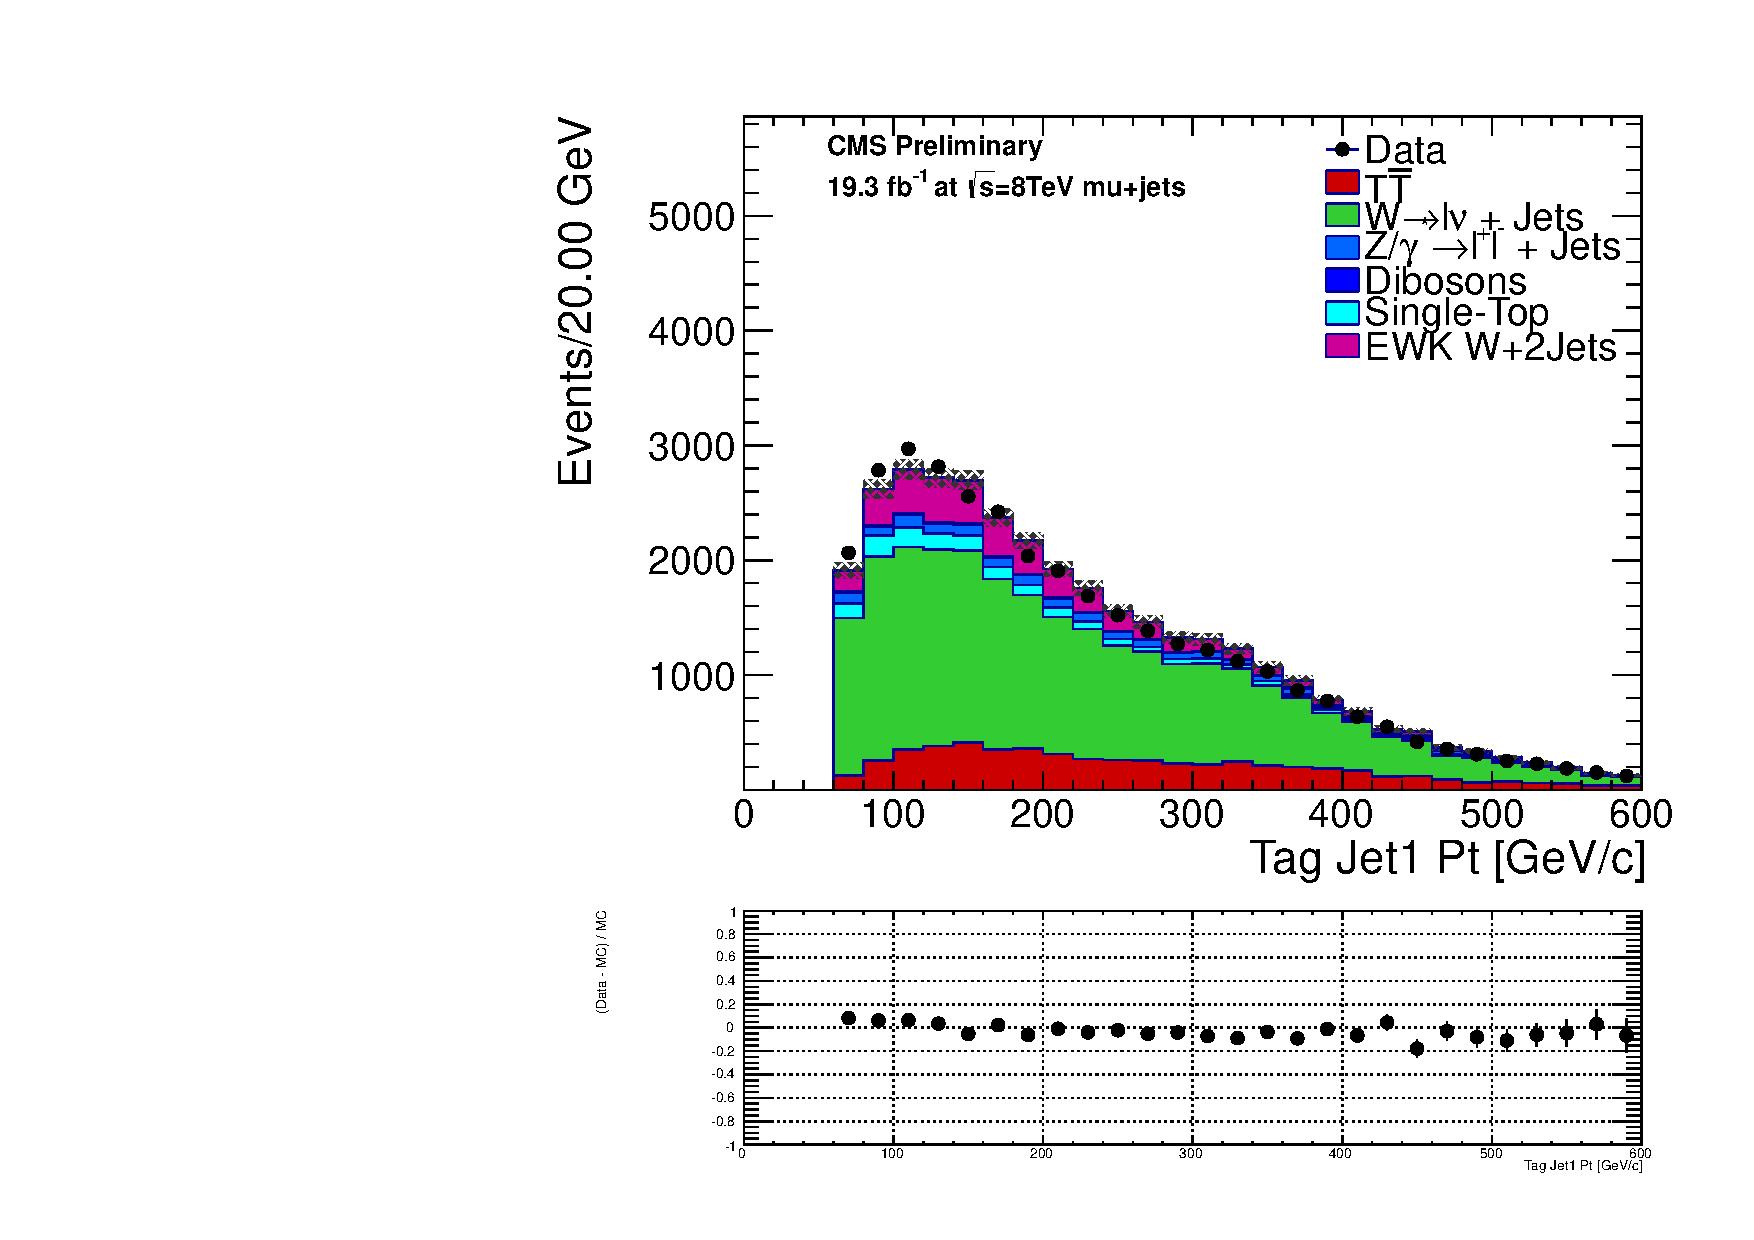
\includegraphics[width=0.49\textwidth]{figs/n-1_plots_mu/mu_EWK_W_2jets_tagjet1_pt_mjj_600_tagjet1_60_tagjet2_50_Zeppenfield_1point2_EWKW2jets.pdf}
    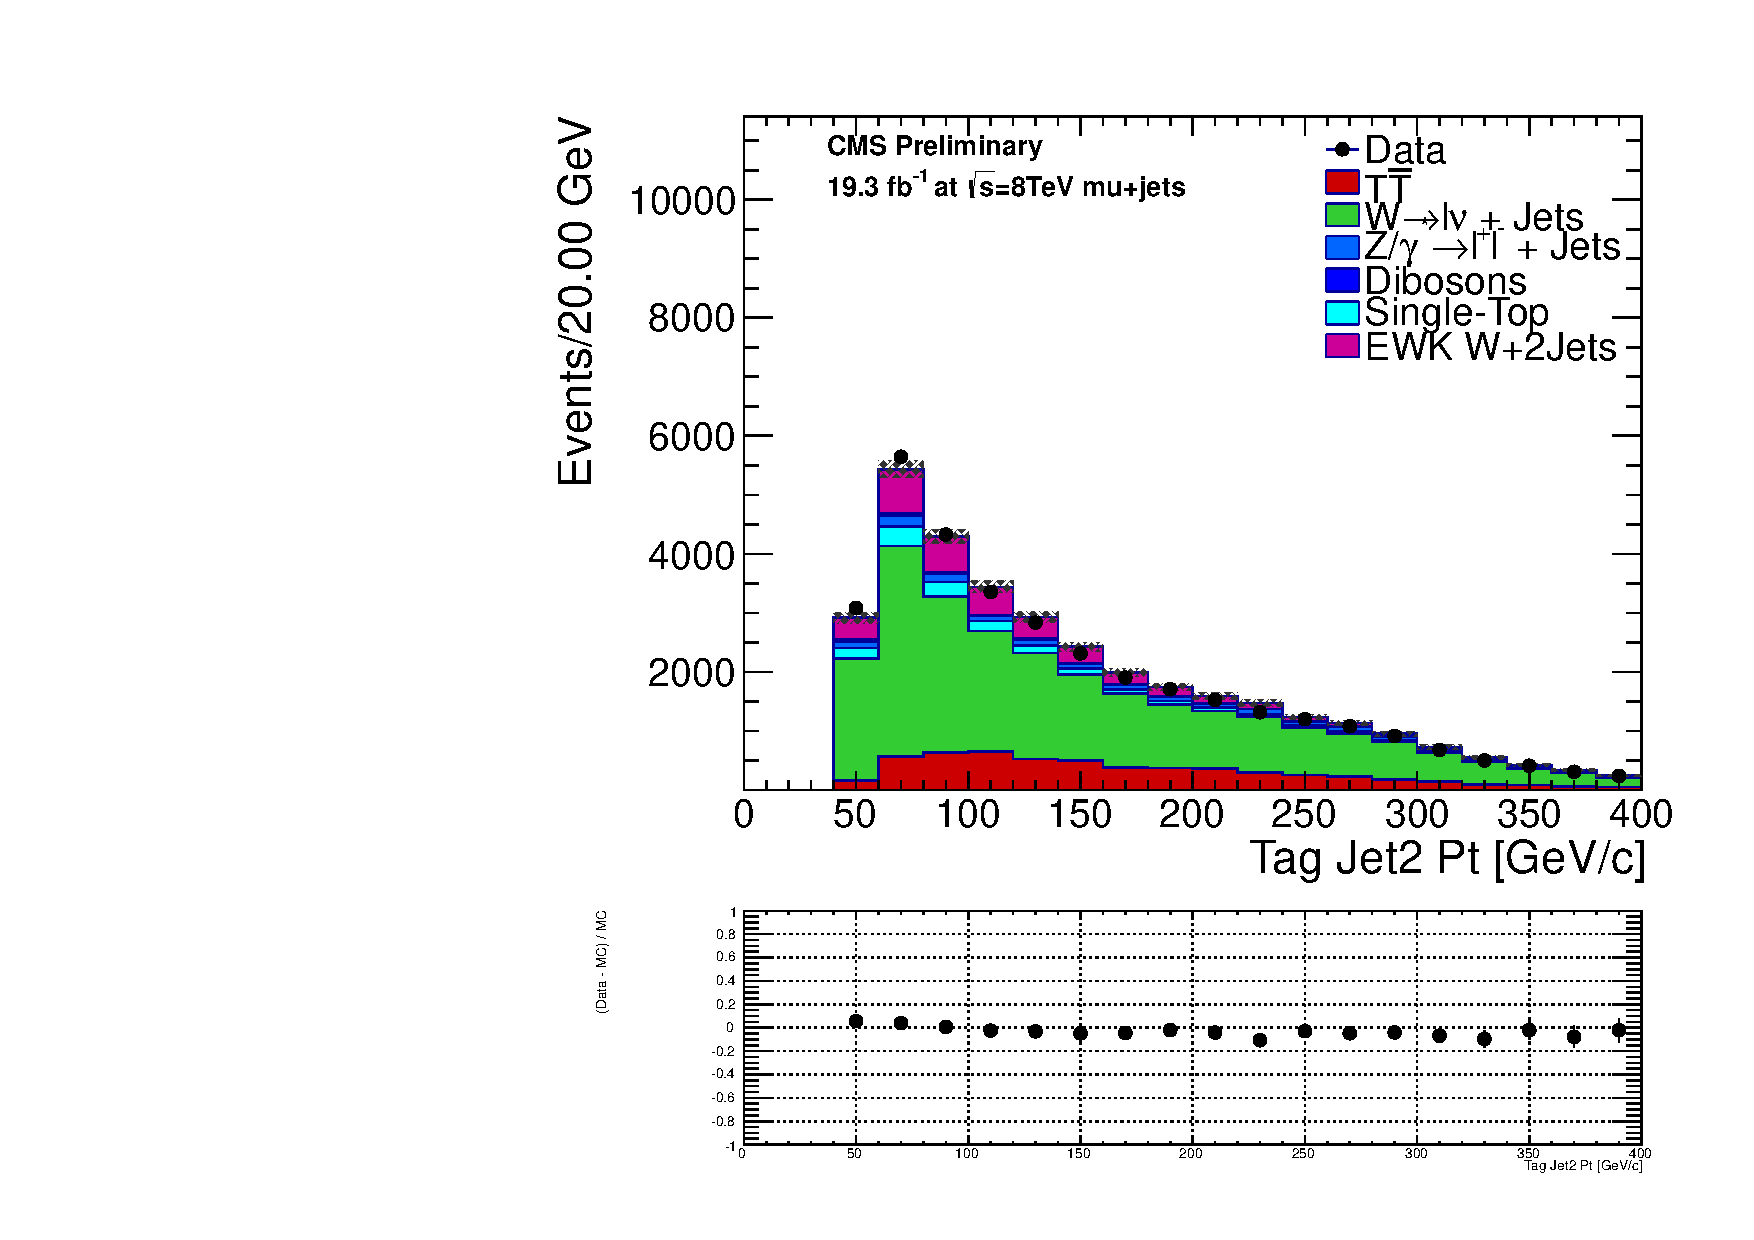
\includegraphics[width=0.49\textwidth]{figs/n-1_plots_mu/mu_EWK_W_2jets_tagjet2_pt_mjj_600_tagjet1_60_tagjet2_50_Zeppenfield_1point2_EWKW2jets.pdf}
    \caption{Comparison of the leading jet (left) and 
      the second leading jet (right) $p_{T}$ distributions from data and MC for the muon+jets
      selection.}
    \label{fig:mu_jet_pt}}
\end{figure}
%%%%%%%%%%%%%%%%%%%%%%%%%%%%
\begin{figure}[h!t]
  {\centering
    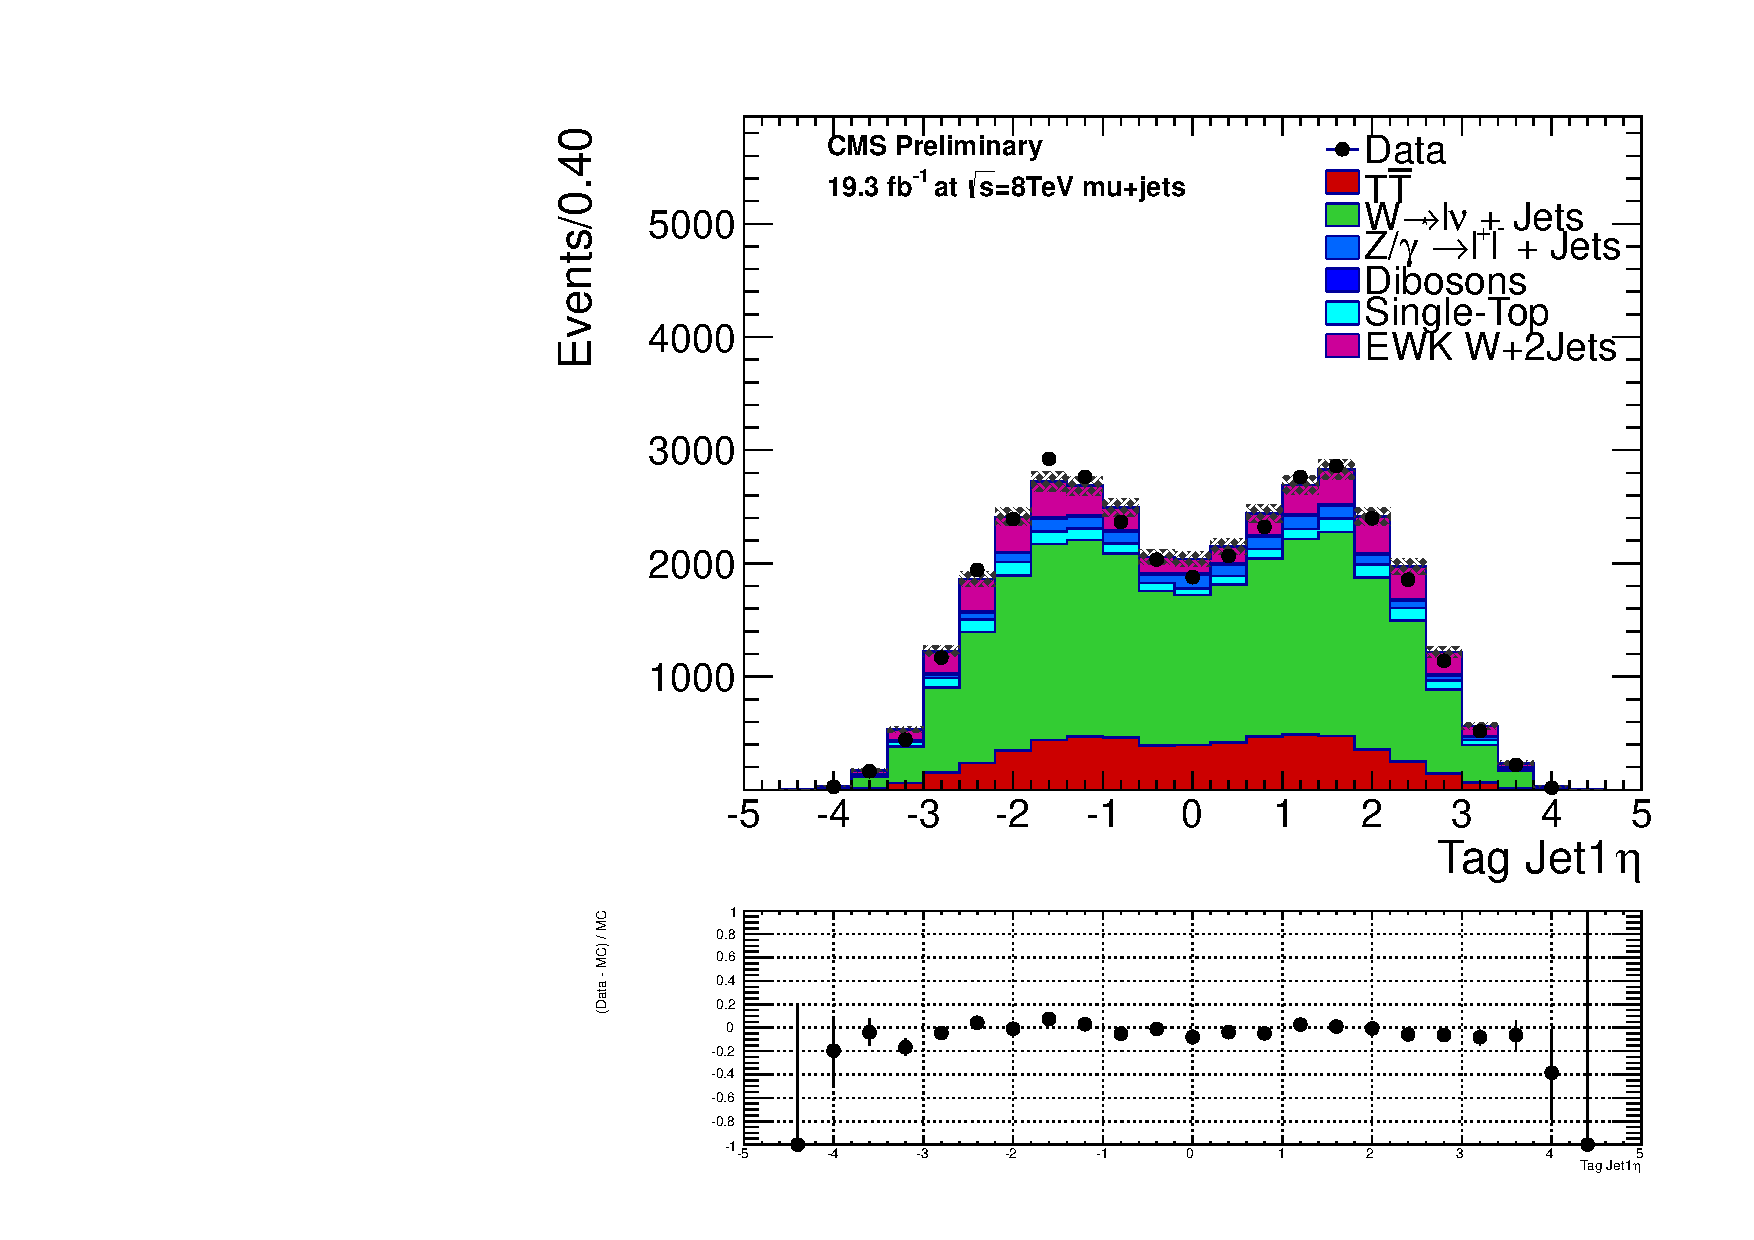
\includegraphics[width=0.49\textwidth]{figs/n-1_plots_mu/mu_EWK_W_2jets_tagjet1_eta_mjj_600_tagjet1_60_tagjet2_50_Zeppenfield_1point2_EWKW2jets.pdf}
    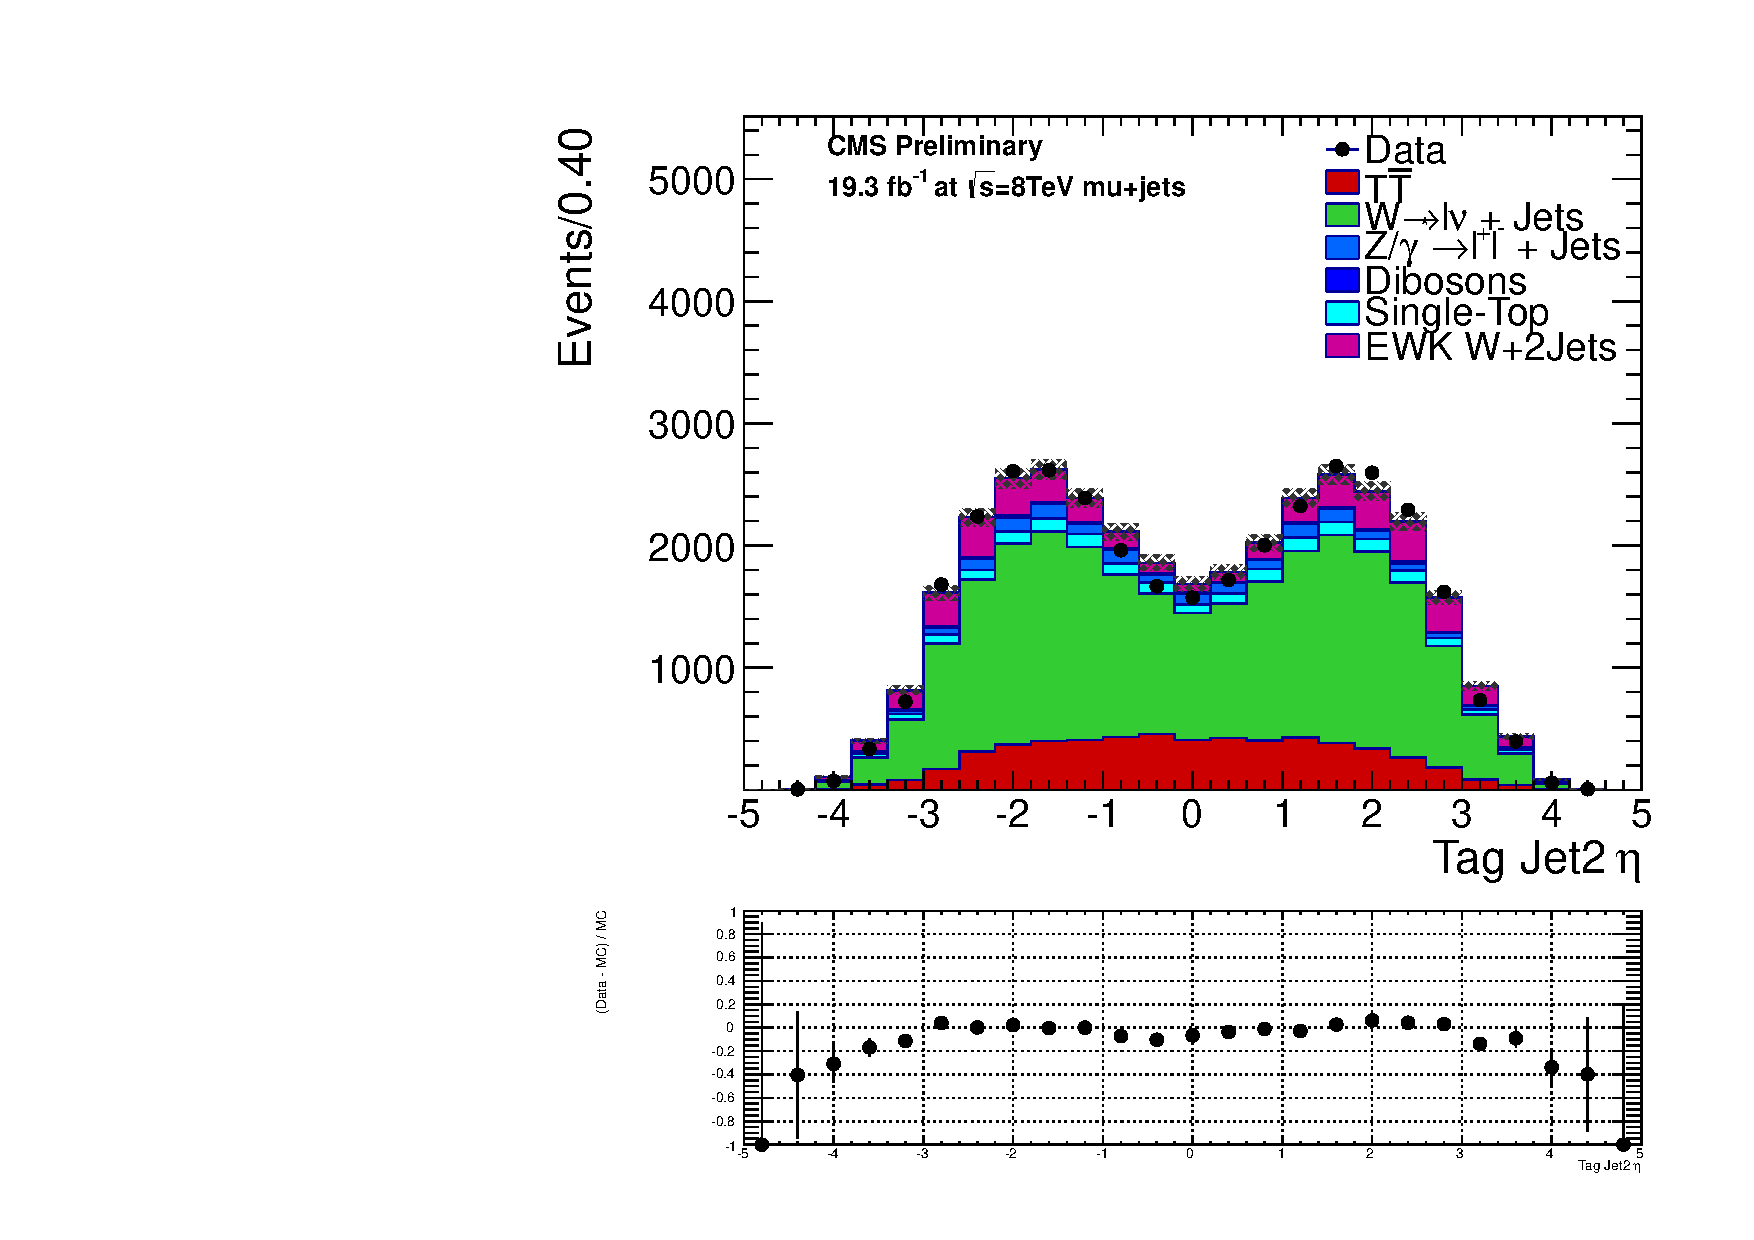
\includegraphics[width=0.49\textwidth]{figs/n-1_plots_mu/mu_EWK_W_2jets_tagjet2_eta_mjj_600_tagjet1_60_tagjet2_50_Zeppenfield_1point2_EWKW2jets.pdf}
    \caption{Comparison of the leading jet $\eta $ (left) and the
    second leading jet $\eta $ (right) distributions from data and MC
    for the muon+jets selection. }
\label{fig:mu_jet_eta}}
\end{figure}
%%%%%%%%%%%%%%%%%%%%%%%%%%%%
\begin{figure}[h!t]
  {\centering
    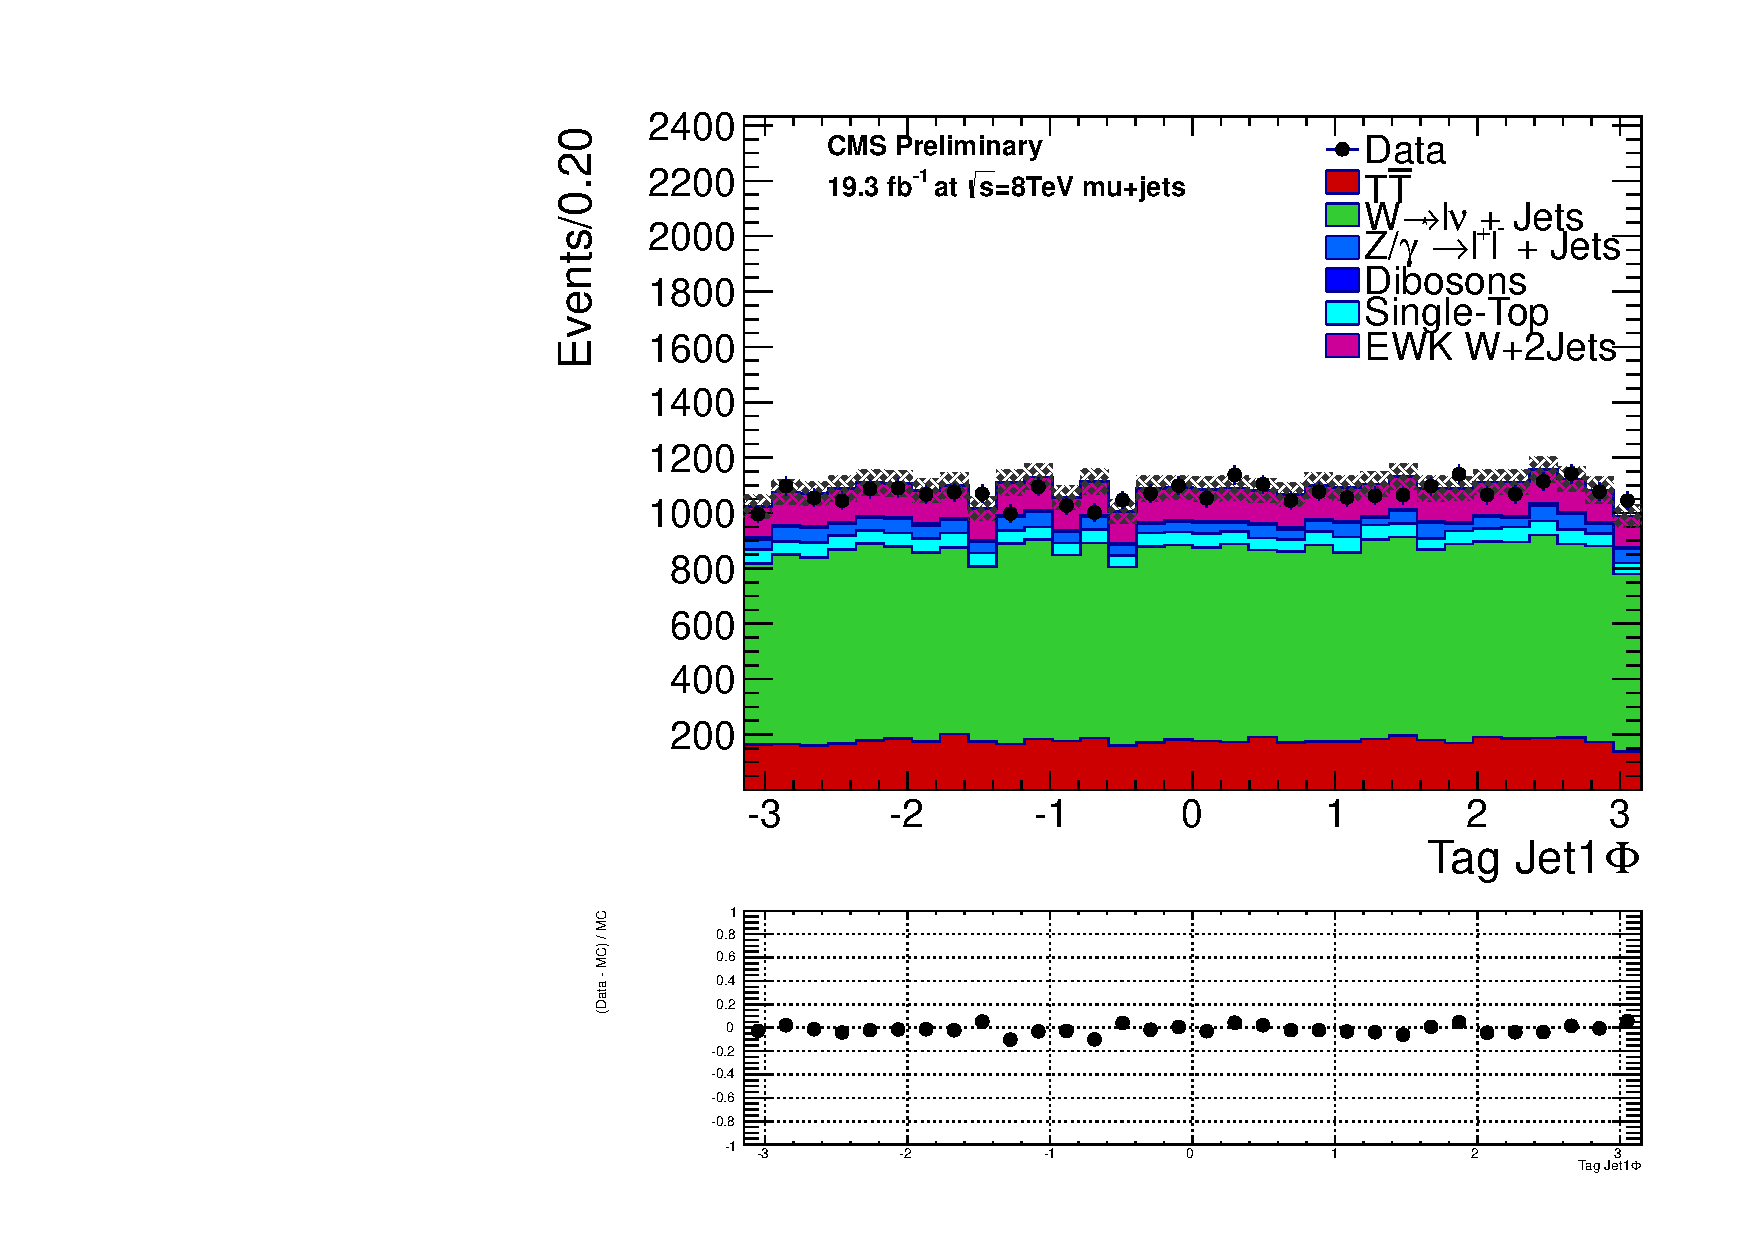
\includegraphics[width=0.49\textwidth]{figs/n-1_plots_mu/mu_EWK_W_2jets_tagjet1_phi_mjj_600_tagjet1_60_tagjet2_50_Zeppenfield_1point2_EWKW2jets.pdf}
    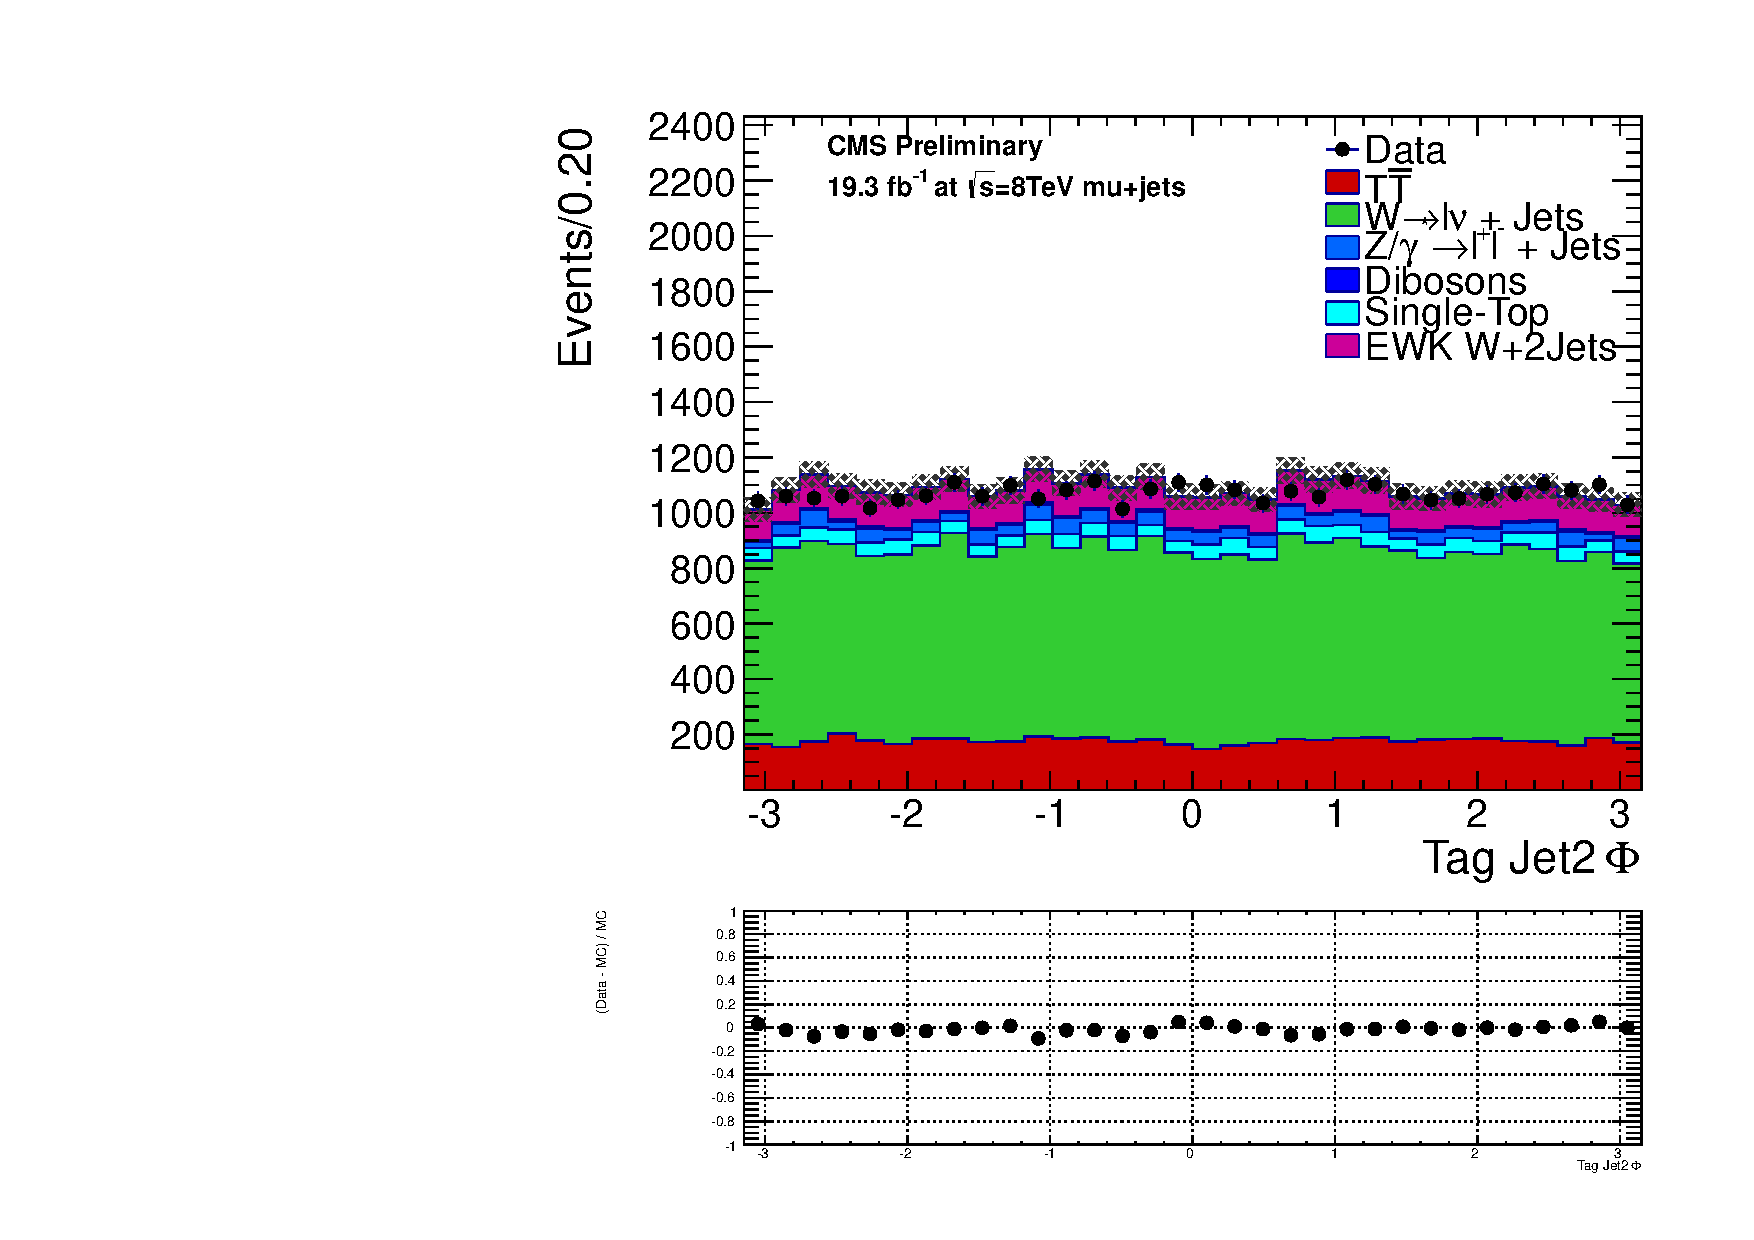
\includegraphics[width=0.49\textwidth]{figs/n-1_plots_mu/mu_EWK_W_2jets_tagjet2_phi_mjj_600_tagjet1_60_tagjet2_50_Zeppenfield_1point2_EWKW2jets.pdf}
    \caption{Comparison of the leading jet $\phi $ (left) and the
    second leading jet $\phi $ (right) distributions from data and MC
    for the muon+jets selection. }
\label{fig:mu_jet_phi}}
\end{figure}
%%%%%%%%%%%%%%%%%%%%%%%%%%%%
\begin{figure}[h!t]
  {\centering
    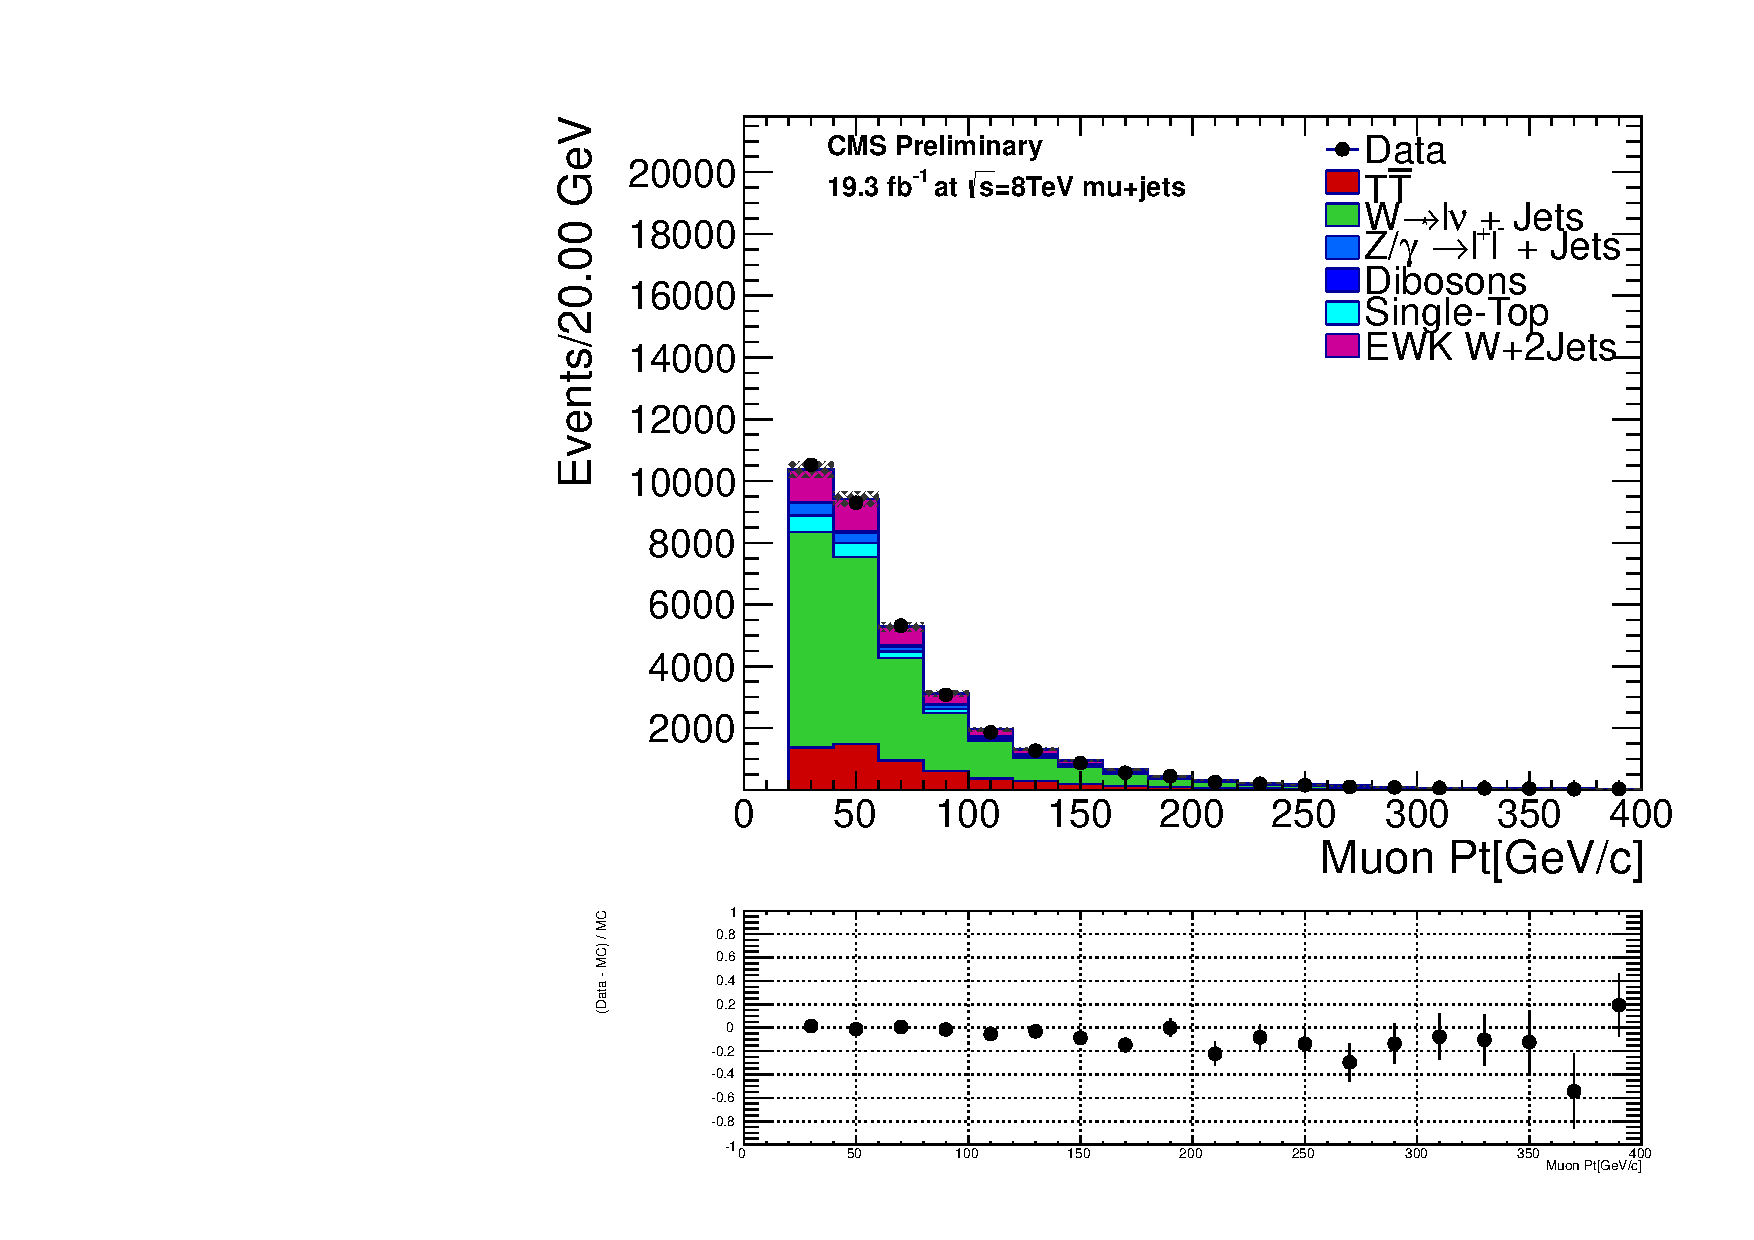
\includegraphics[width=0.49\textwidth]{figs/n-1_plots_mu/mu_EWK_W_2jets_l_pt_mjj_600_tagjet1_60_tagjet2_50_Zeppenfield_1point2_EWKW2jets.pdf}
    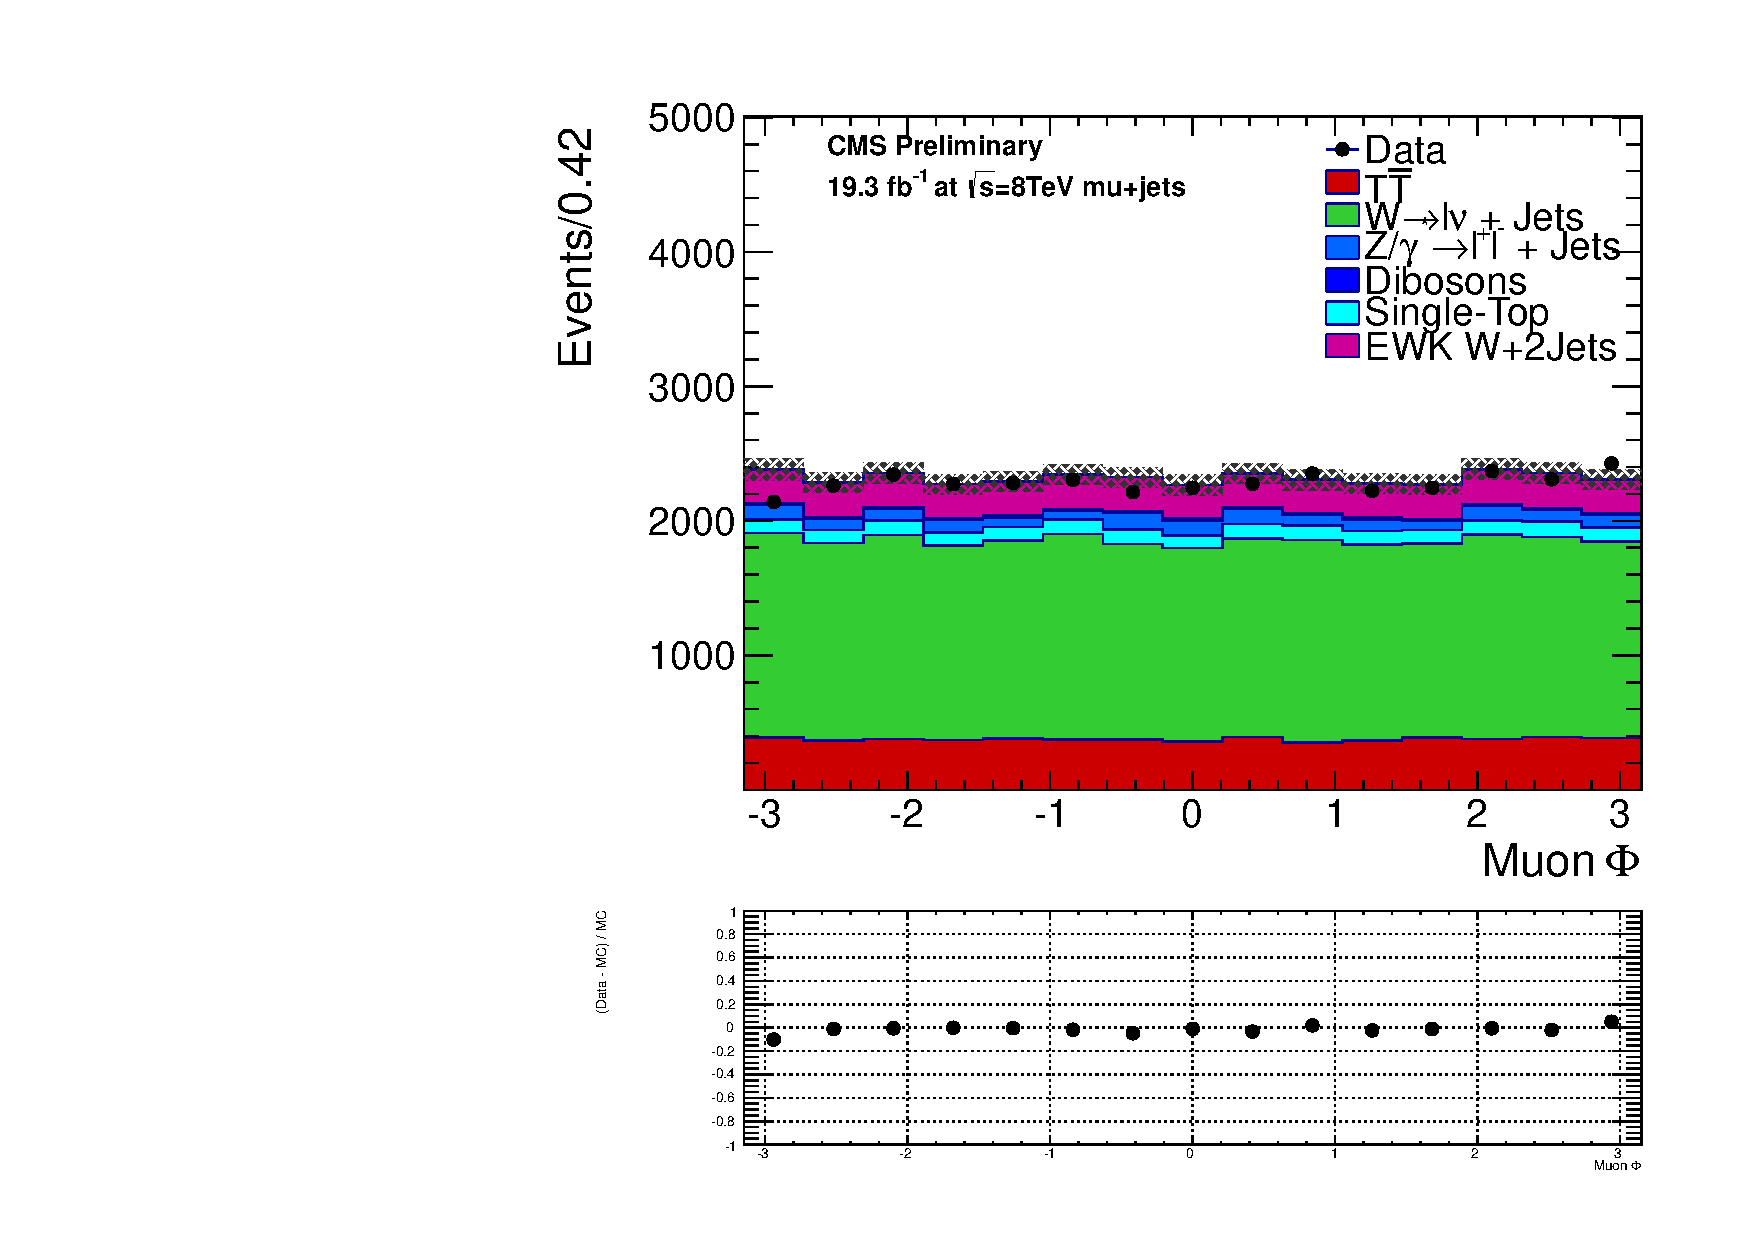
\includegraphics[width=0.49\textwidth]{figs/n-1_plots_mu/mu_EWK_W_2jets_l_phi_mjj_600_tagjet1_60_tagjet2_50_Zeppenfield_1point2_EWKW2jets.pdf}
    \caption{Comparison of the muon $p_{T} $ (left) and the muon
      $\phi $ (right) distributions from data and MC for the muon+jets selection.
      }
    \label{fig:mu_muon_phi}}
\end{figure}
%%%%%%%%%%%%%%%%%%%%%%%%%%%%
\begin{figure}[h!t]
  {\centering
    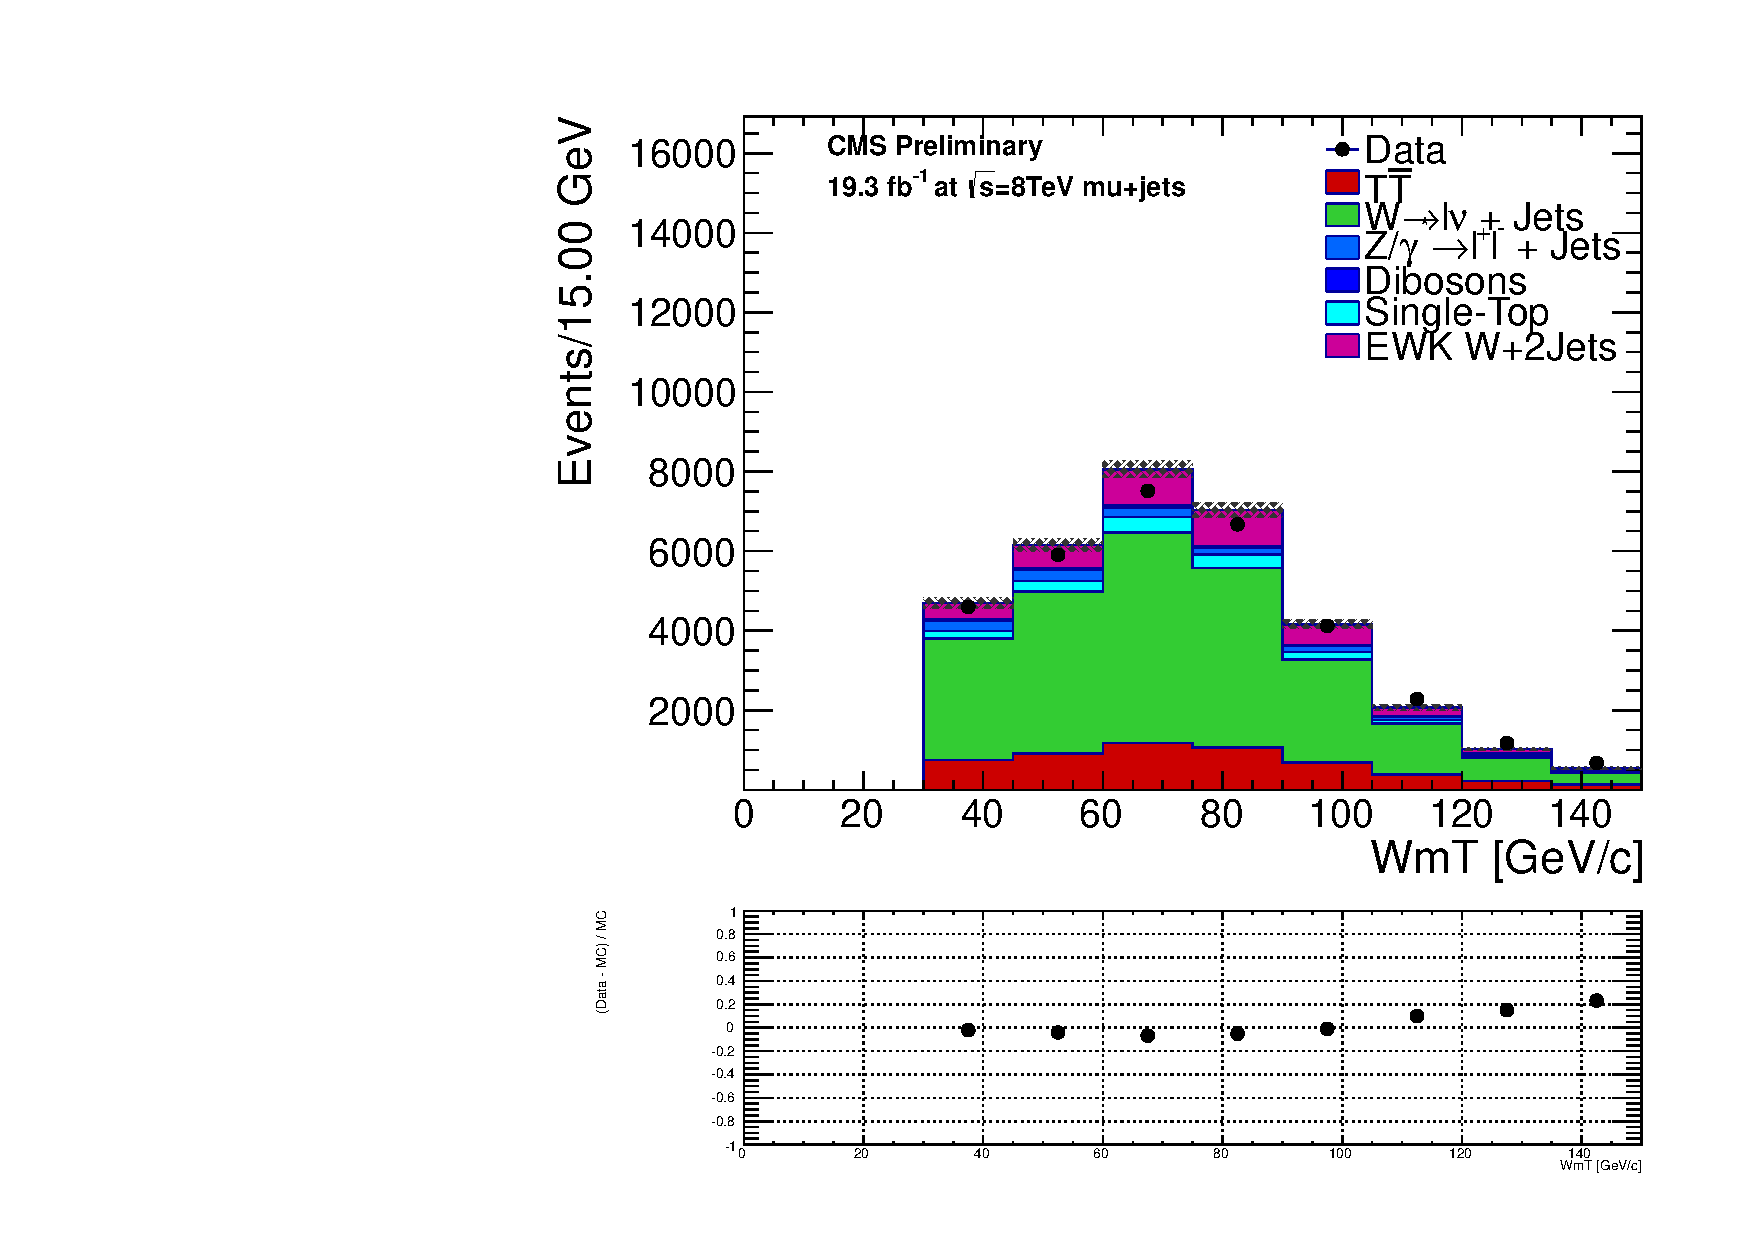
\includegraphics[width=0.49\textwidth]{figs/n-1_plots_mu/mu_EWK_W_2jets_W_mT_mjj_600_tagjet1_60_tagjet2_50_Zeppenfield_1point2_EWKW2jets.pdf}
    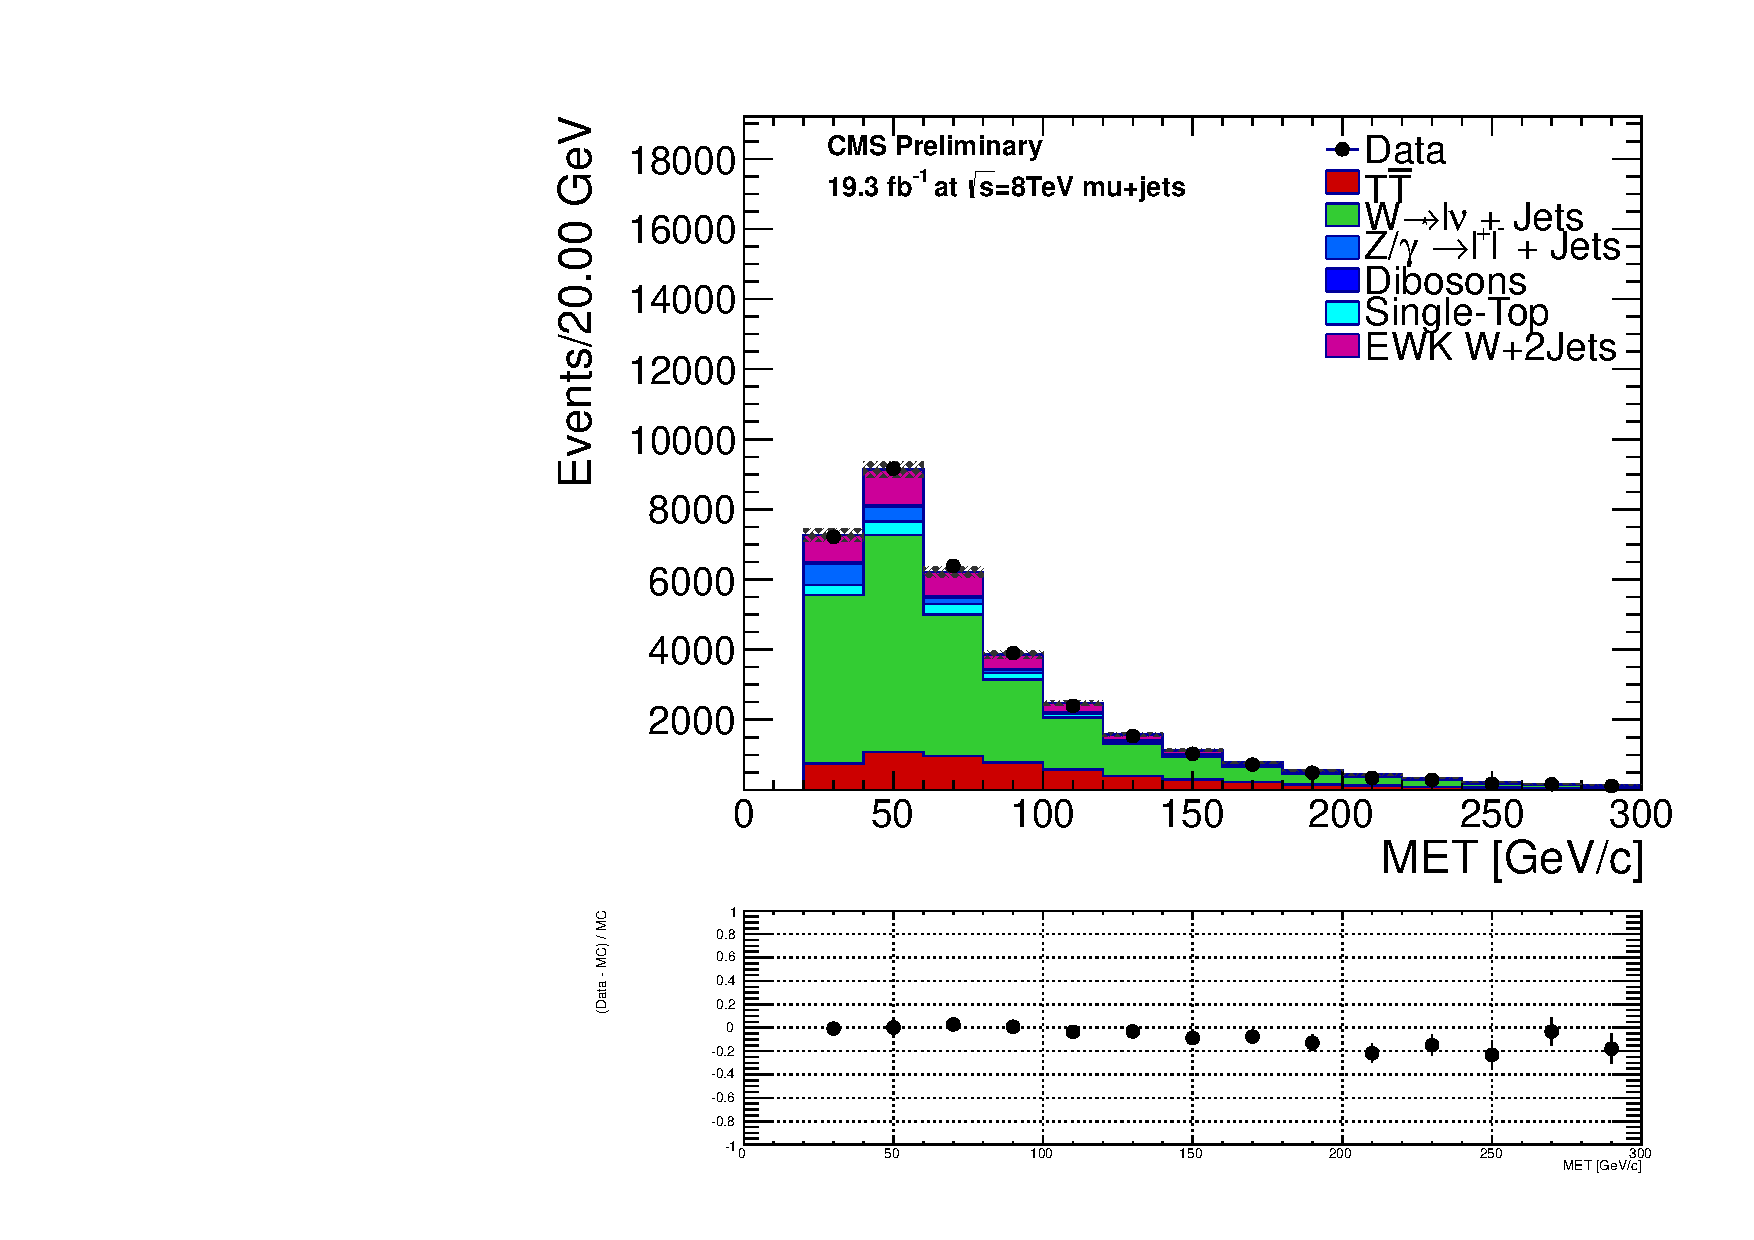
\includegraphics[width=0.49\textwidth]{figs/n-1_plots_mu/mu_event_met_pfmet_mjj_600_tagjet1_60_tagjet2_50_Zeppenfield_1point2_EWKW2jets.pdf}
    \caption{Comparison of the distributions from data and MC of the
     transverse mass of the muon / MET system (left) and the MET (right)
    for the muon+jets selection. 
    }
    \label{fig:mu_W_Mt}}
\end{figure}
%%%%%%%%%%%%%%%%%%%%%%%%%%%%
%%%%%%%%%%%%%%%%%%%%%%%%%%%%
\begin{figure}[h!t]
  {\centering
    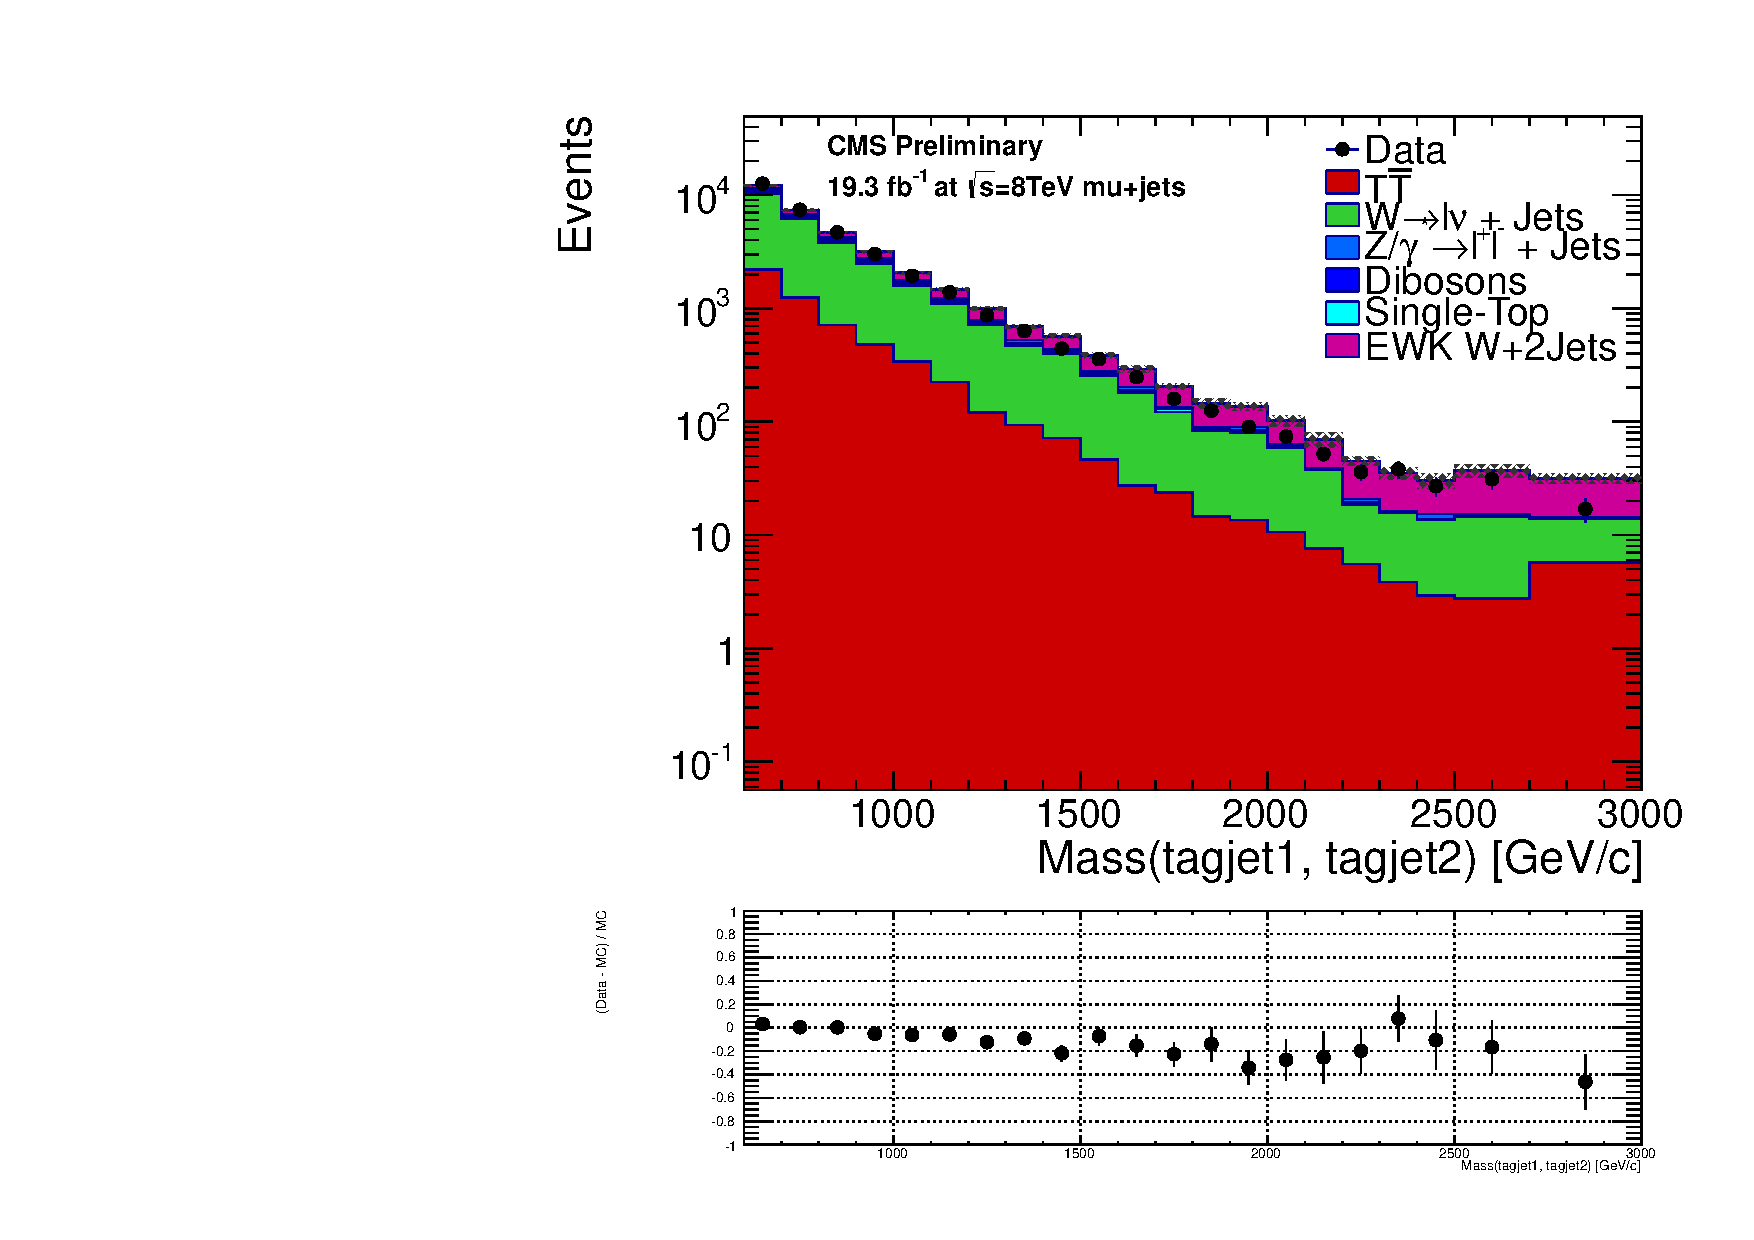
\includegraphics[width=0.49\textwidth]{figs/n-1_plots_mu/mu_EWK_W_2jets_tagjet_mass_mjj_600_tagjet1_60_tagjet2_50_Zeppenfield_1point2_logy_rebin_EWKW2jets.pdf}
    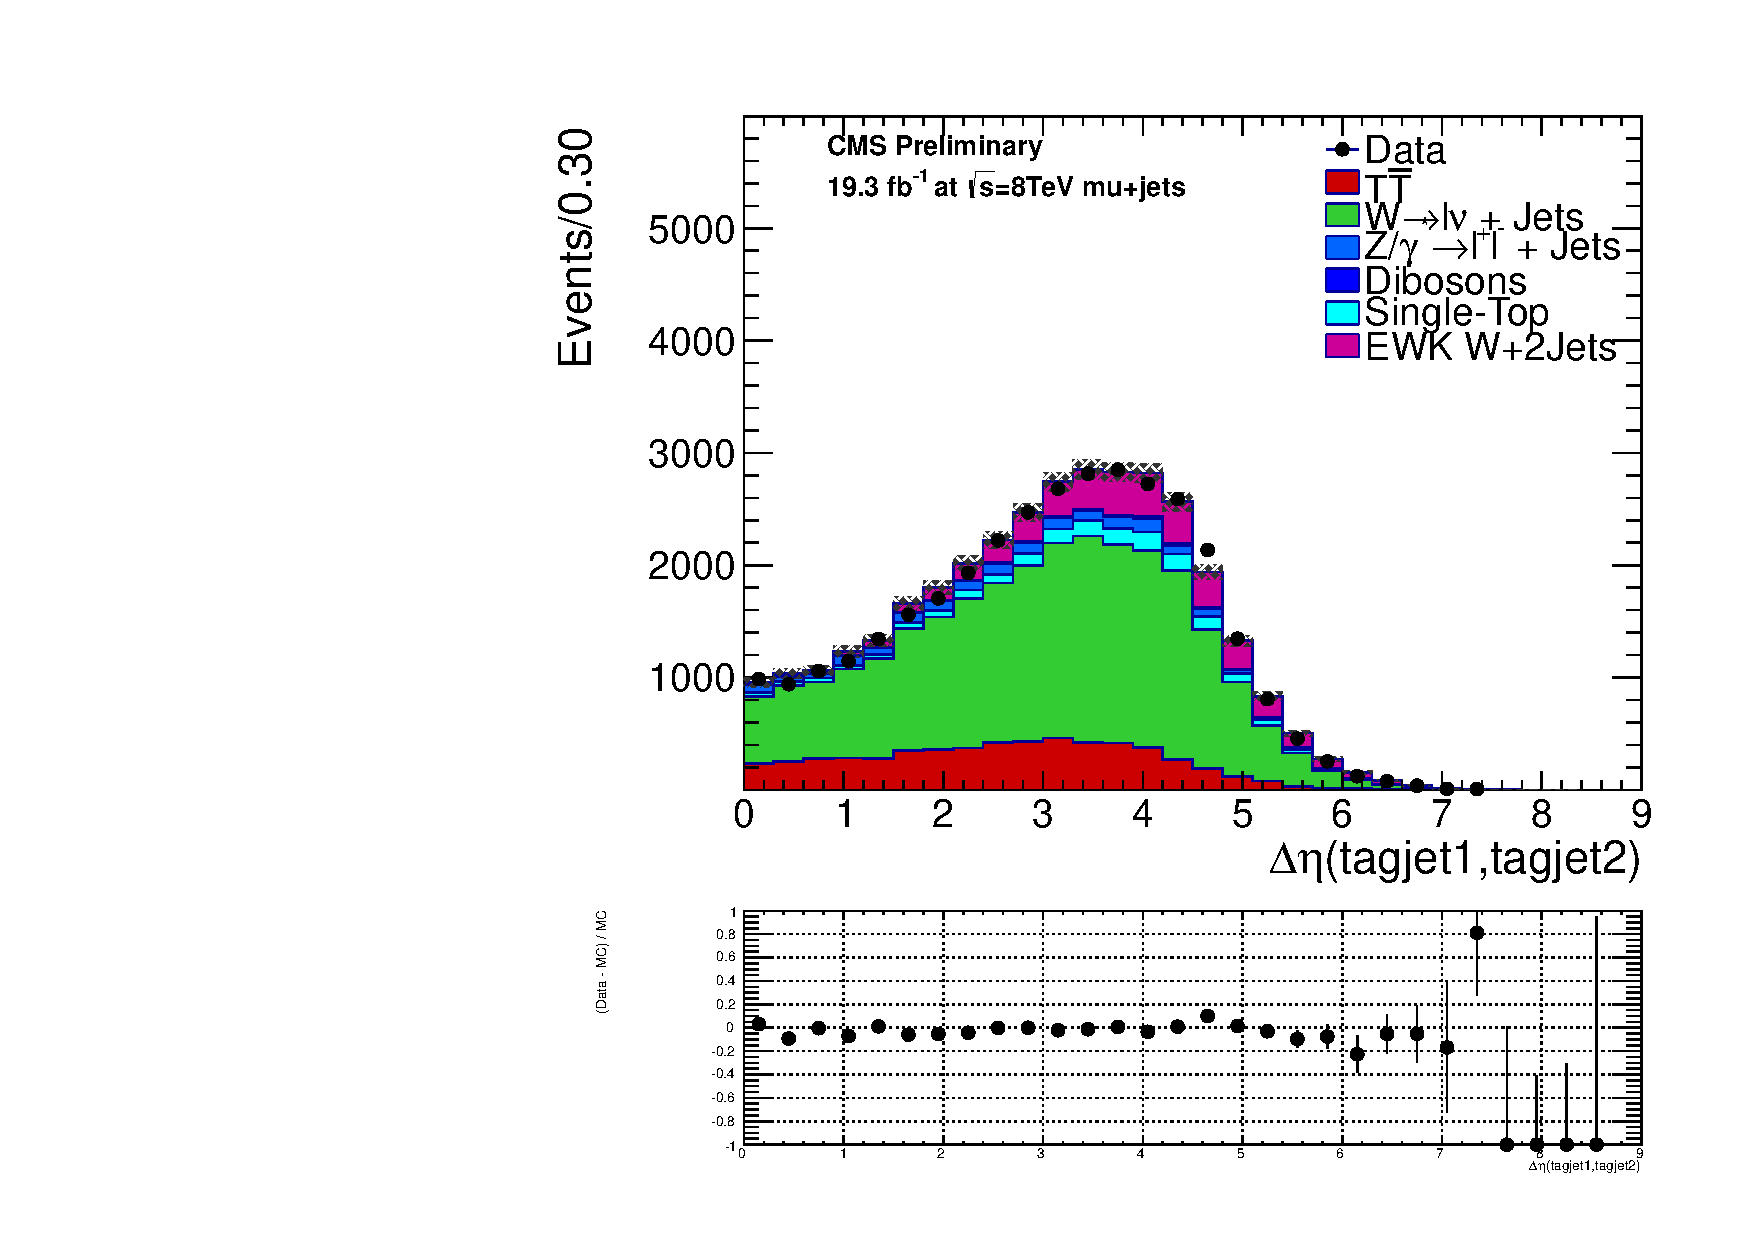
\includegraphics[width=0.49\textwidth]{figs/n-1_plots_mu/mu_EWK_W_2jets_tagjet_deltaeta_mjj_600_tagjet1_60_tagjet2_50_Zeppenfield_1point2_EWKW2jets.pdf}
    \caption{Comparison of the distributions from
      data and MC of the tag jet pair invariant mass (left)
      and the $\Delta\eta$ between the two tag jets (right) for the muon+jets selection. 
      }
    \label{fig:mu_dijet}}
\end{figure}
%%%%%%%%%%%%%%%%%%%%%%%%%%%%
\begin{figure}[ht]
{\centering
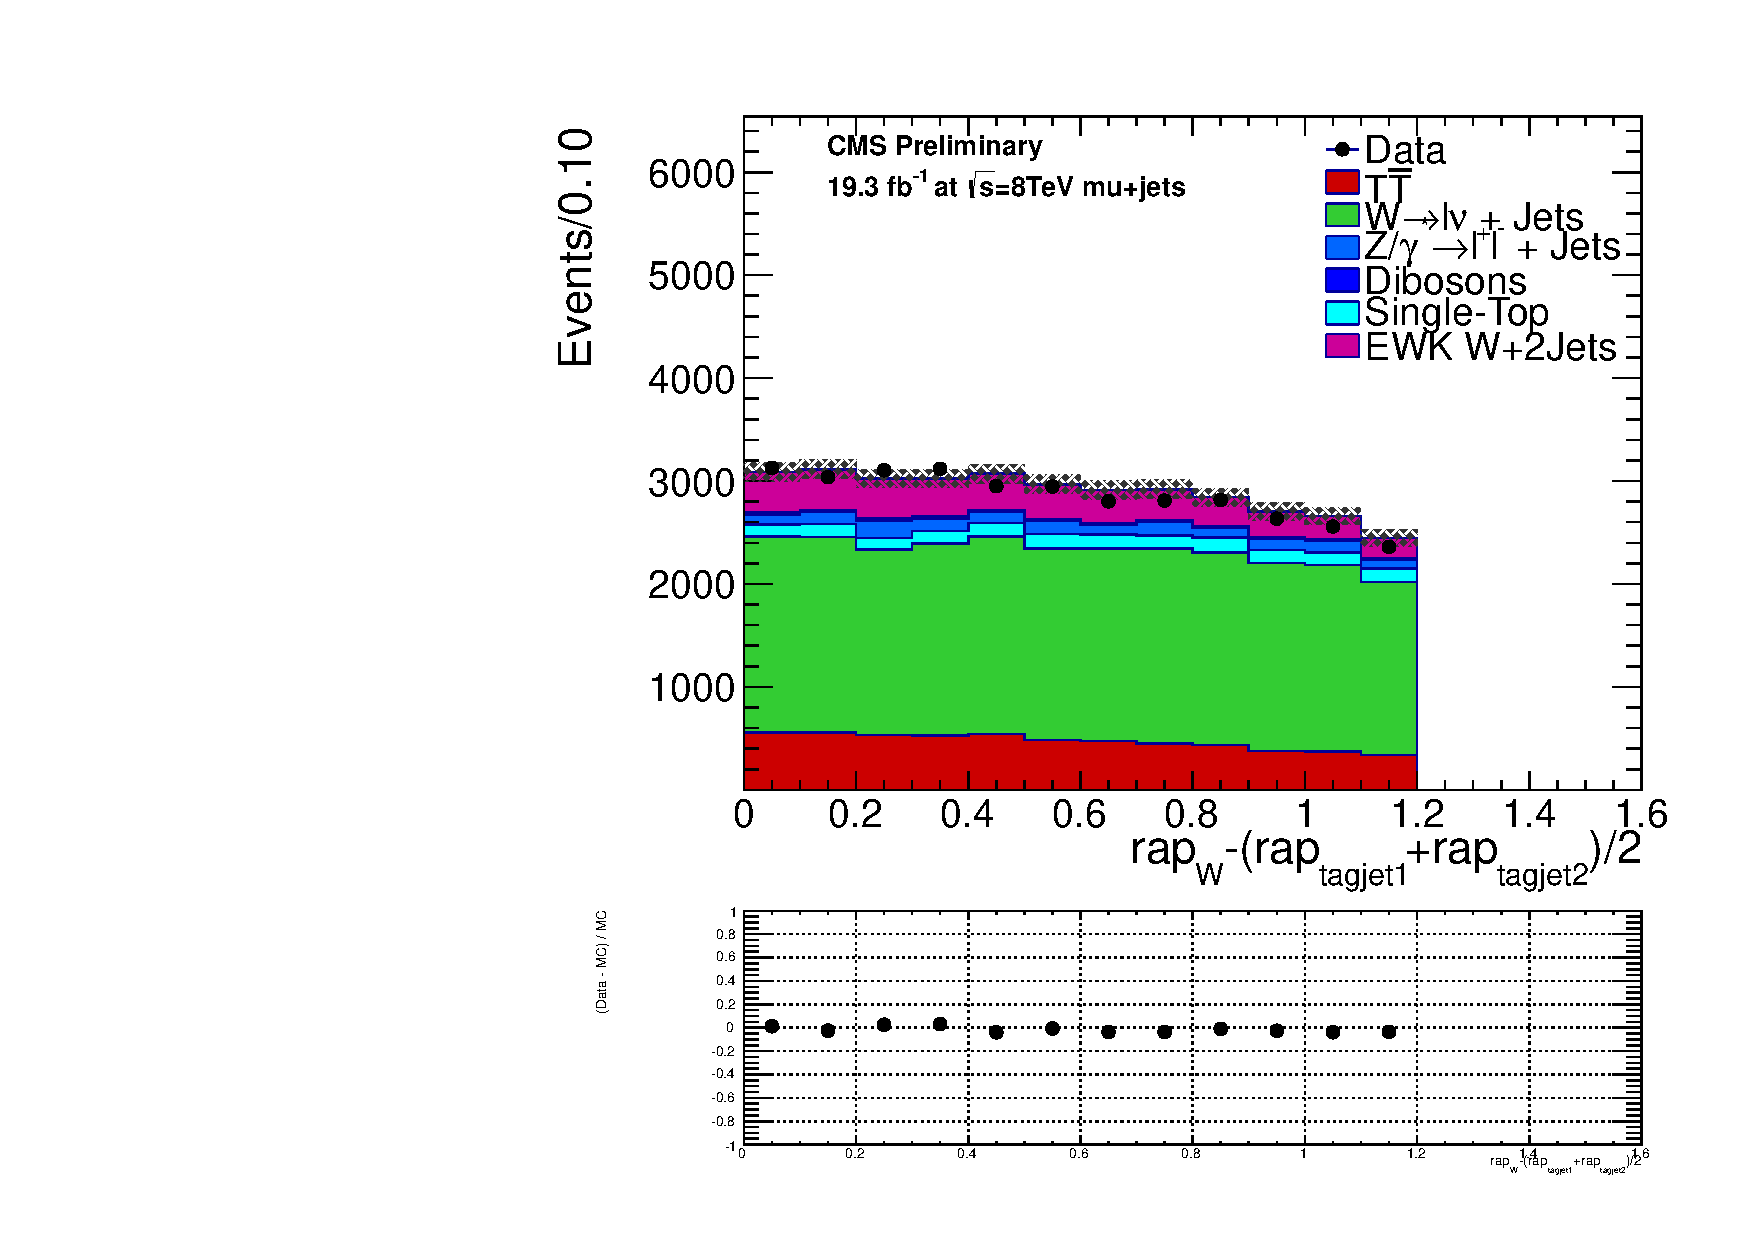
\includegraphics[width=.49\textwidth]{figs/n-1_plots_mu/mu_EWK_W_2jets_W_tagjet_Zeppenfield_mjj_600_tagjet1_60_tagjet2_50_Zeppenfield_1point2_EWKW2jets.pdf}
\caption{Comparison of the distributions from data and MC of the Zeppenfeld variable for muon+jets selection.}
\label{fig:mu_zeppenfield}}
\end{figure}
%%%%%%%%%%%%%%%%%%%%%%%%%%%%
\begin{figure}[h!t]
  {\centering
    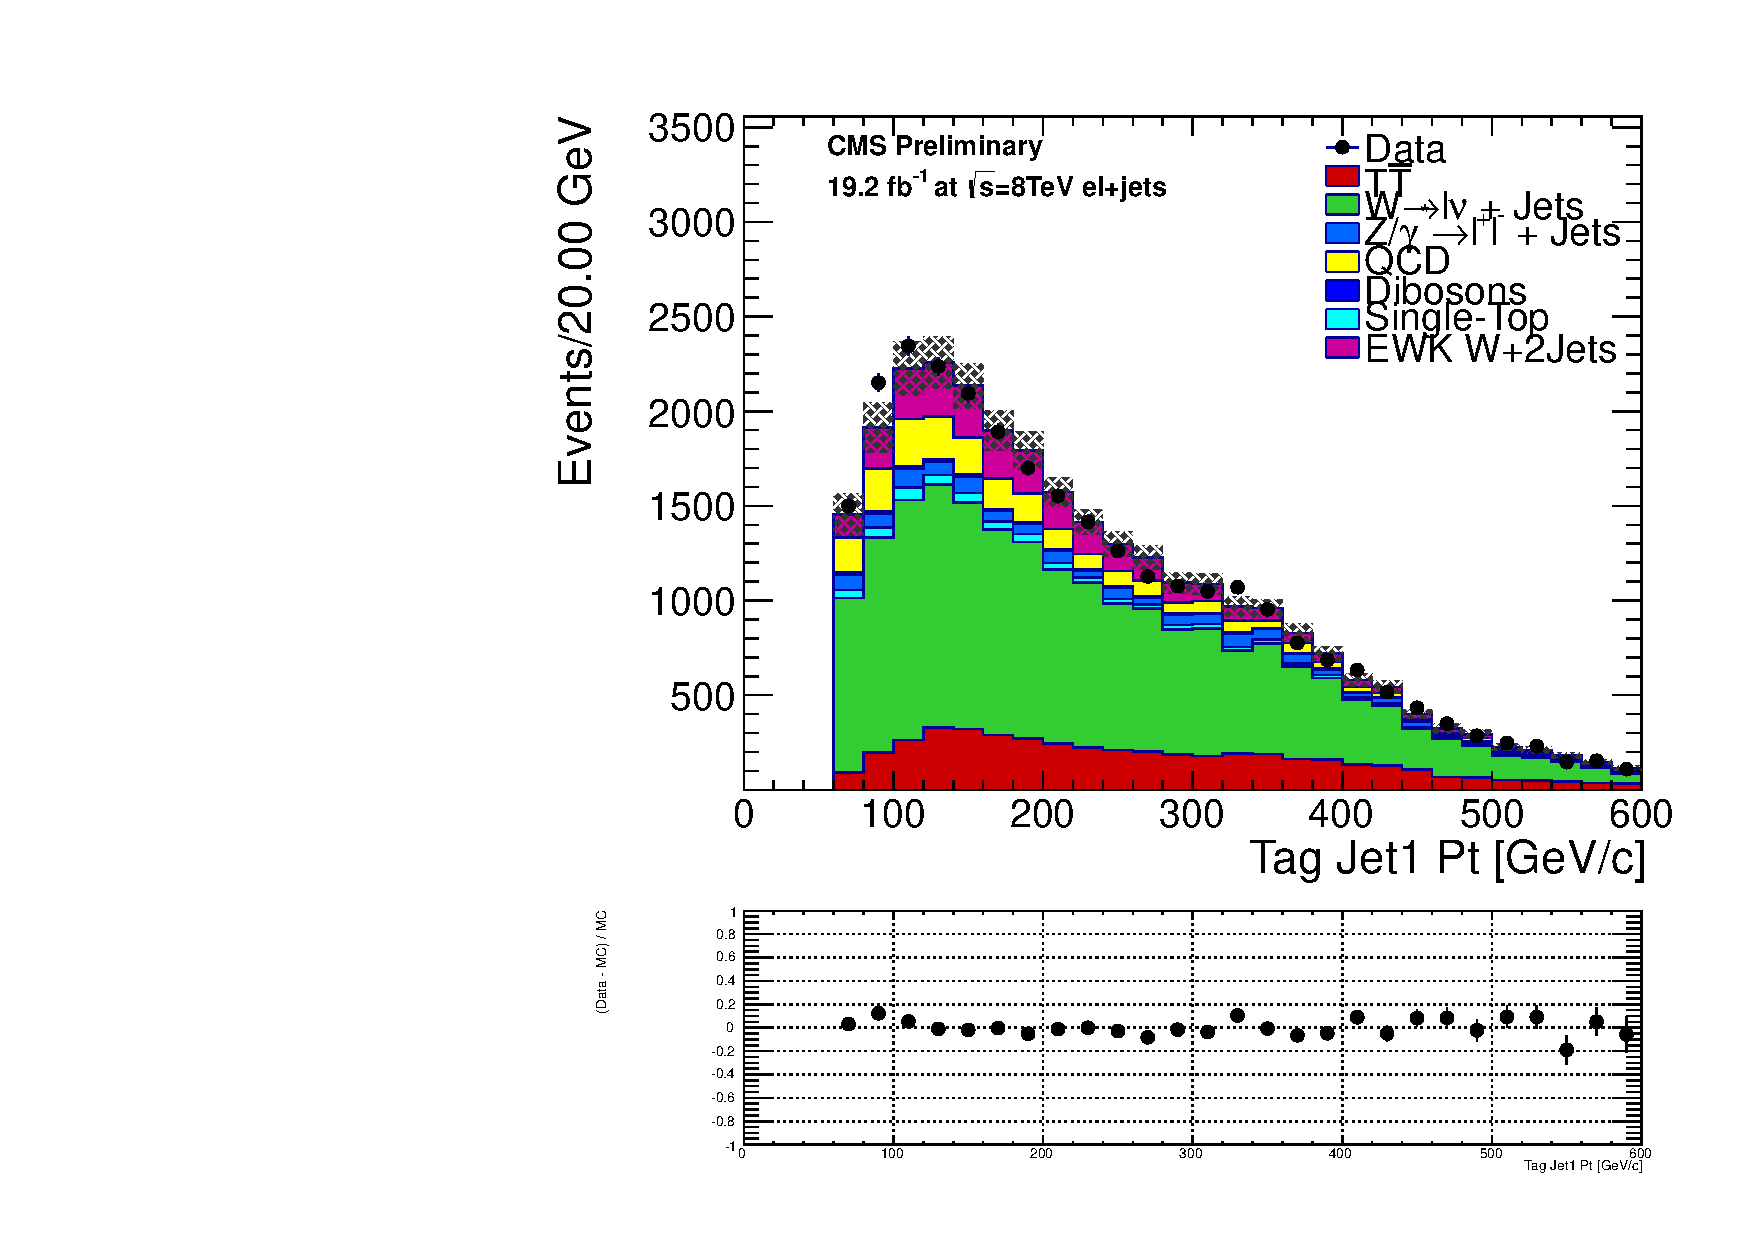
\includegraphics[width=0.49\textwidth]{figs/n-1_plots_el/el_EWK_W_2jets_tagjet1_pt_mjj_600_tagjet1_60_tagjet2_50_Zeppenfield_1point2_met_30_WmT_30_EWKW2jets.pdf}
    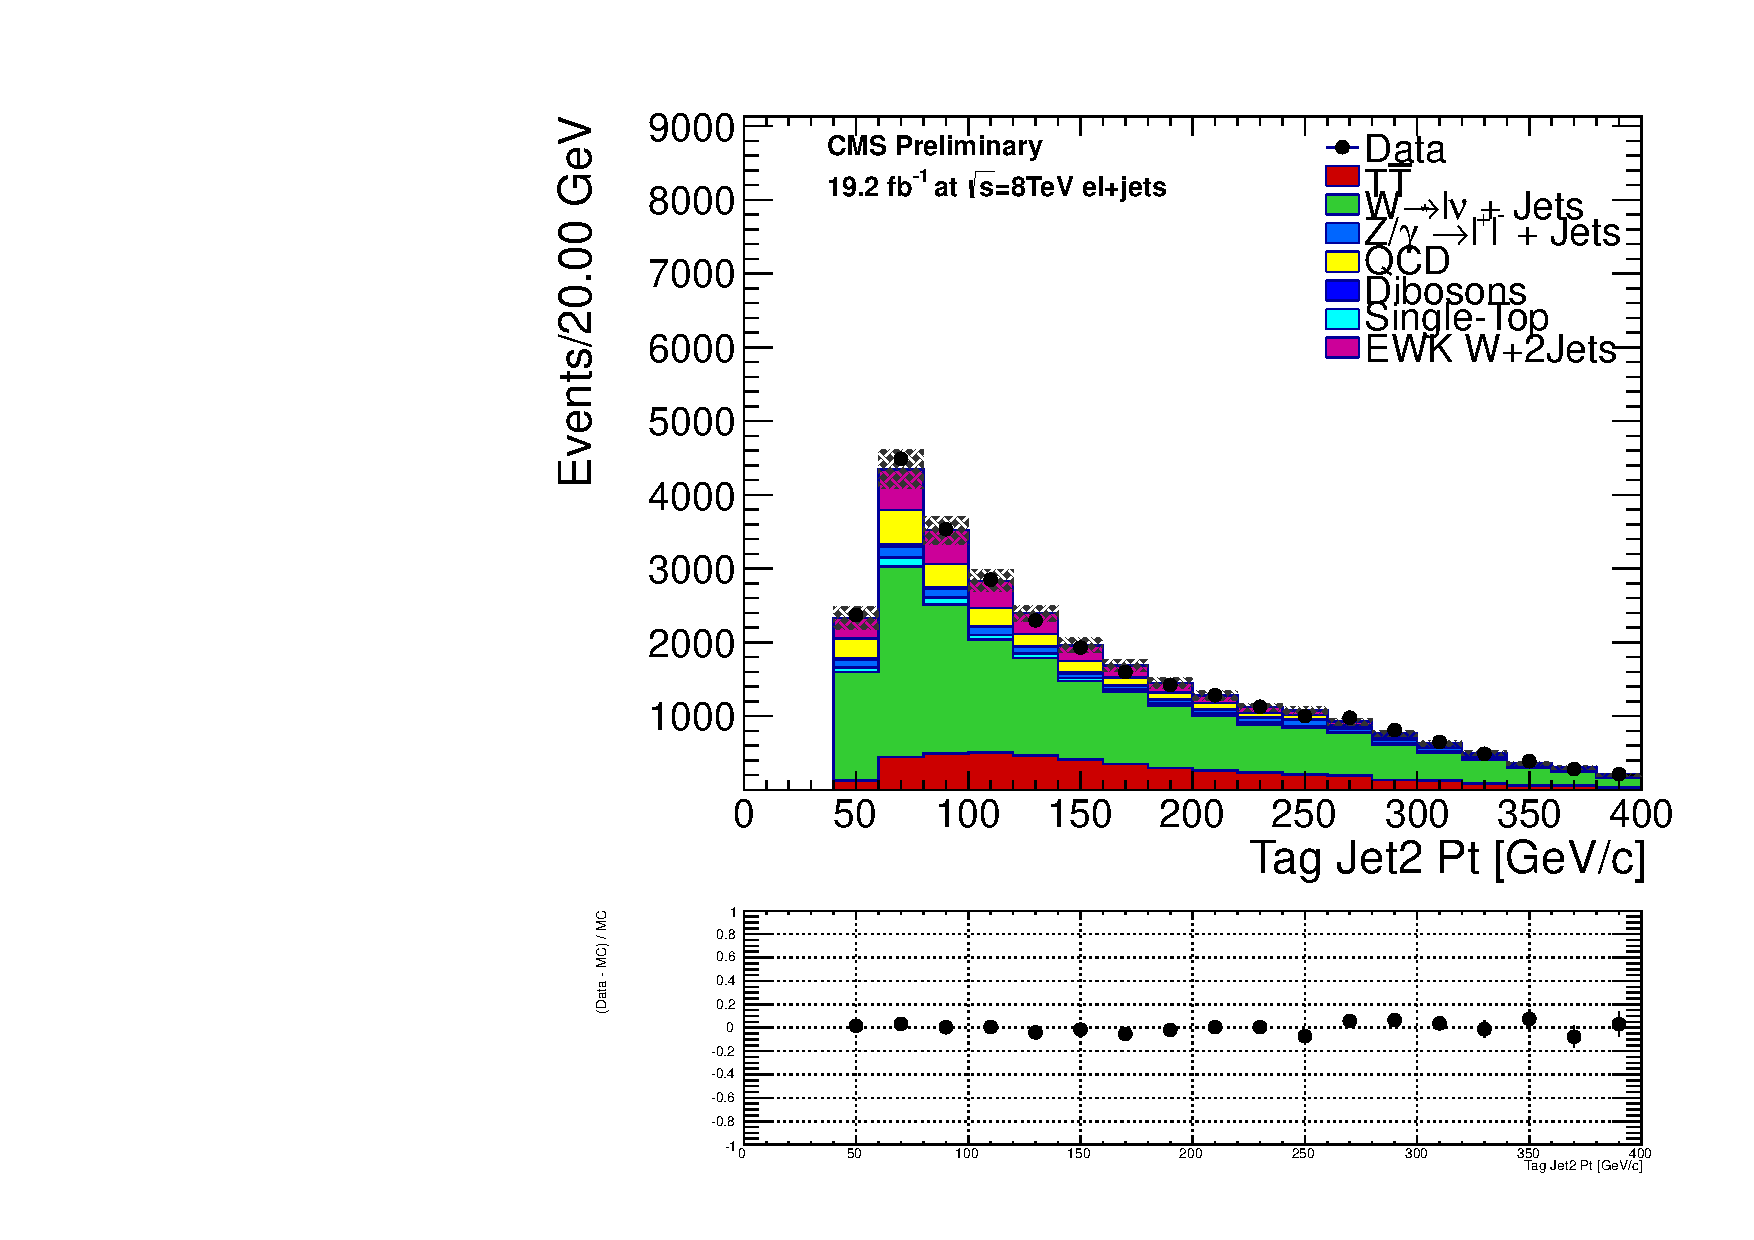
\includegraphics[width=0.49\textwidth]{figs/n-1_plots_el/el_EWK_W_2jets_tagjet2_pt_mjj_600_tagjet1_60_tagjet2_50_Zeppenfield_1point2_met_30_WmT_30_EWKW2jets.pdf}
    \caption{Comparison of the leading jet $p_{T} $ (left) and the
      second leading jet $p_{T} $ (right) distributions from data and MC
      for the electron+jets selection. 
      }
    \label{fig:elec_jet_pt}}
\end{figure}
%%%%%%%%%%%%%%%%%%%%%%%%%%%%
\begin{figure}[h!t]
  {\centering
    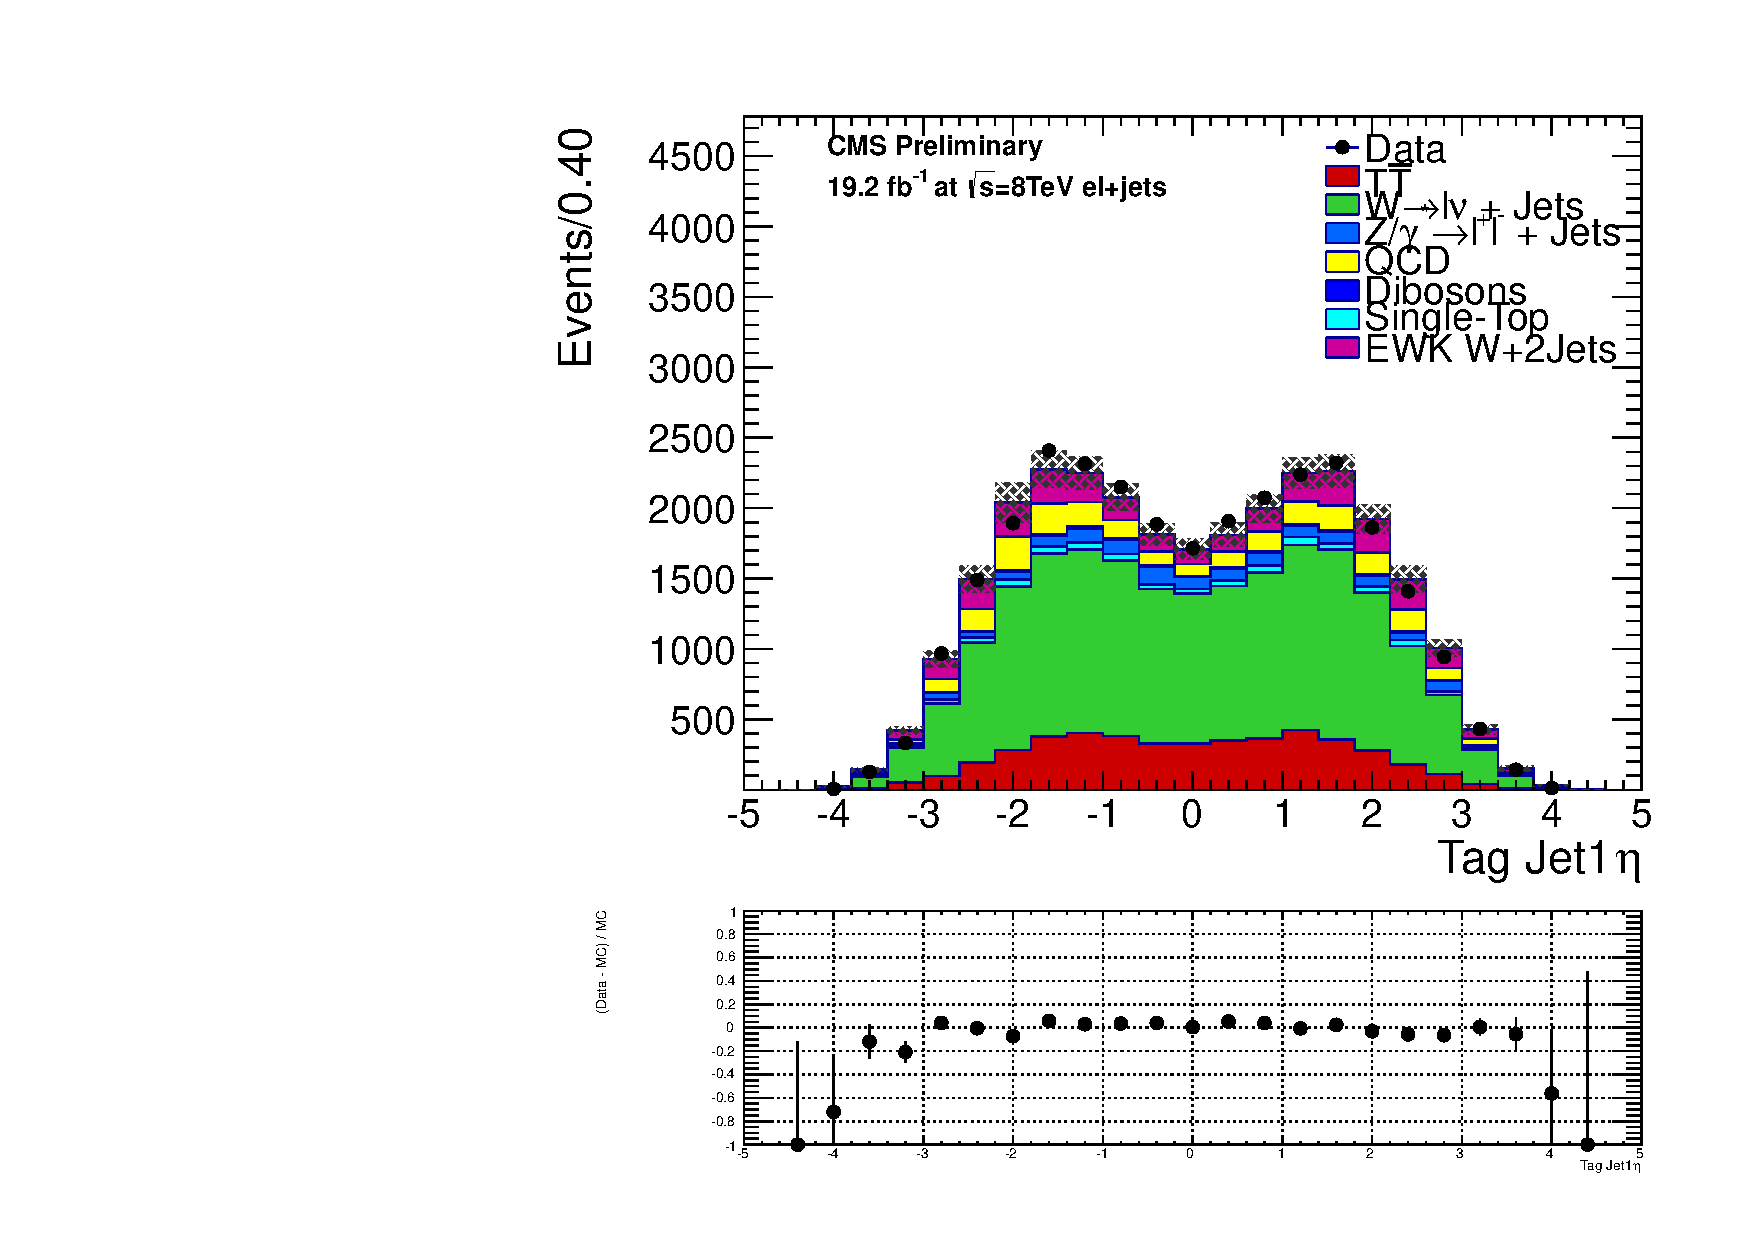
\includegraphics[width=0.49\textwidth]{figs/n-1_plots_el/el_EWK_W_2jets_tagjet1_eta_mjj_600_tagjet1_60_tagjet2_50_Zeppenfield_1point2_met_30_WmT_30_EWKW2jets.pdf}
    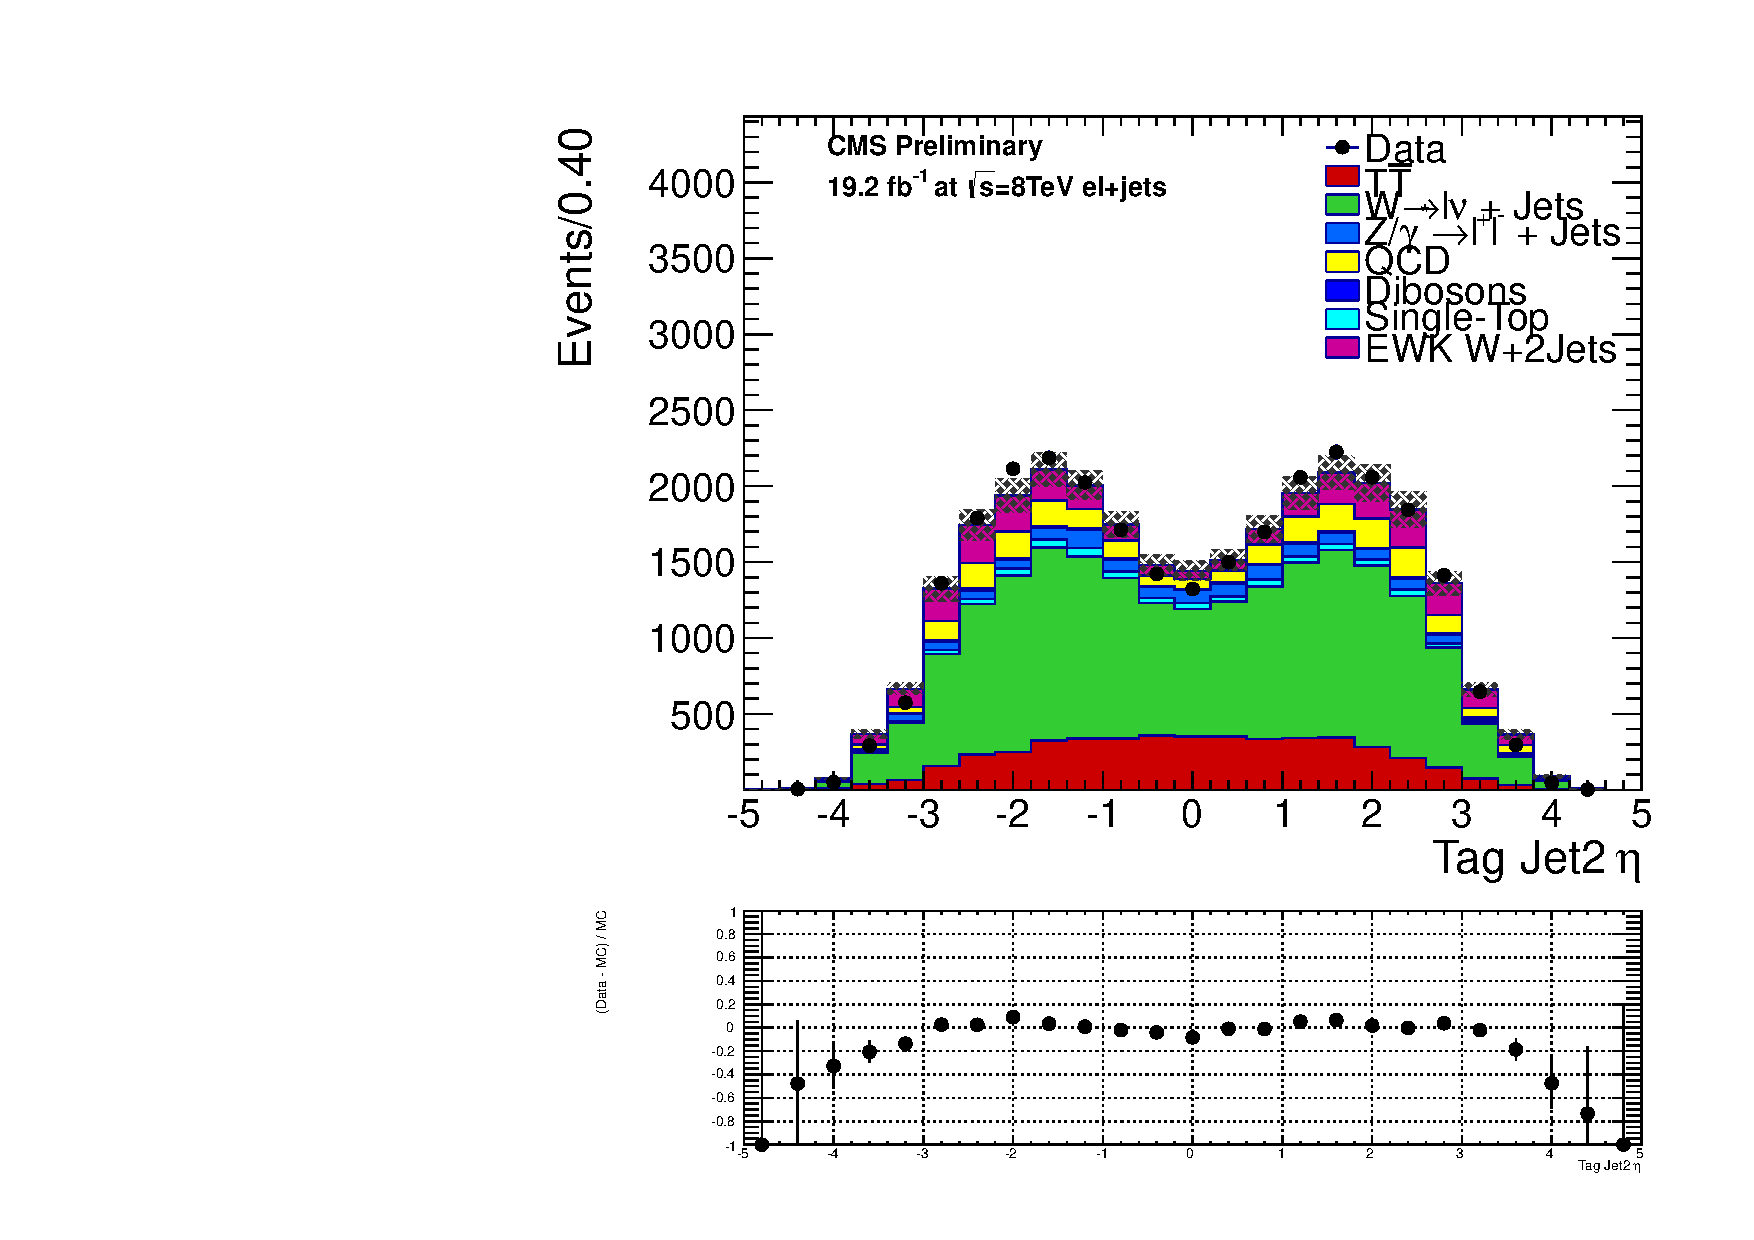
\includegraphics[width=0.49\textwidth]{figs/n-1_plots_el/el_EWK_W_2jets_tagjet2_eta_mjj_600_tagjet1_60_tagjet2_50_Zeppenfield_1point2_met_30_WmT_30_EWKW2jets.pdf}
    \caption{Comparison of the leading jet $\eta $ (left) and the
      second leading jet $\eta $ (right) distributions from data and MC for the electron+jets
      selection. 
      }
    \label{fig:elec_jet_eta}}
\end{figure}
%%%%%%%%%%%%%%%%%%%%%%%%%%%%
\begin{figure}[h!t]
  {\centering
    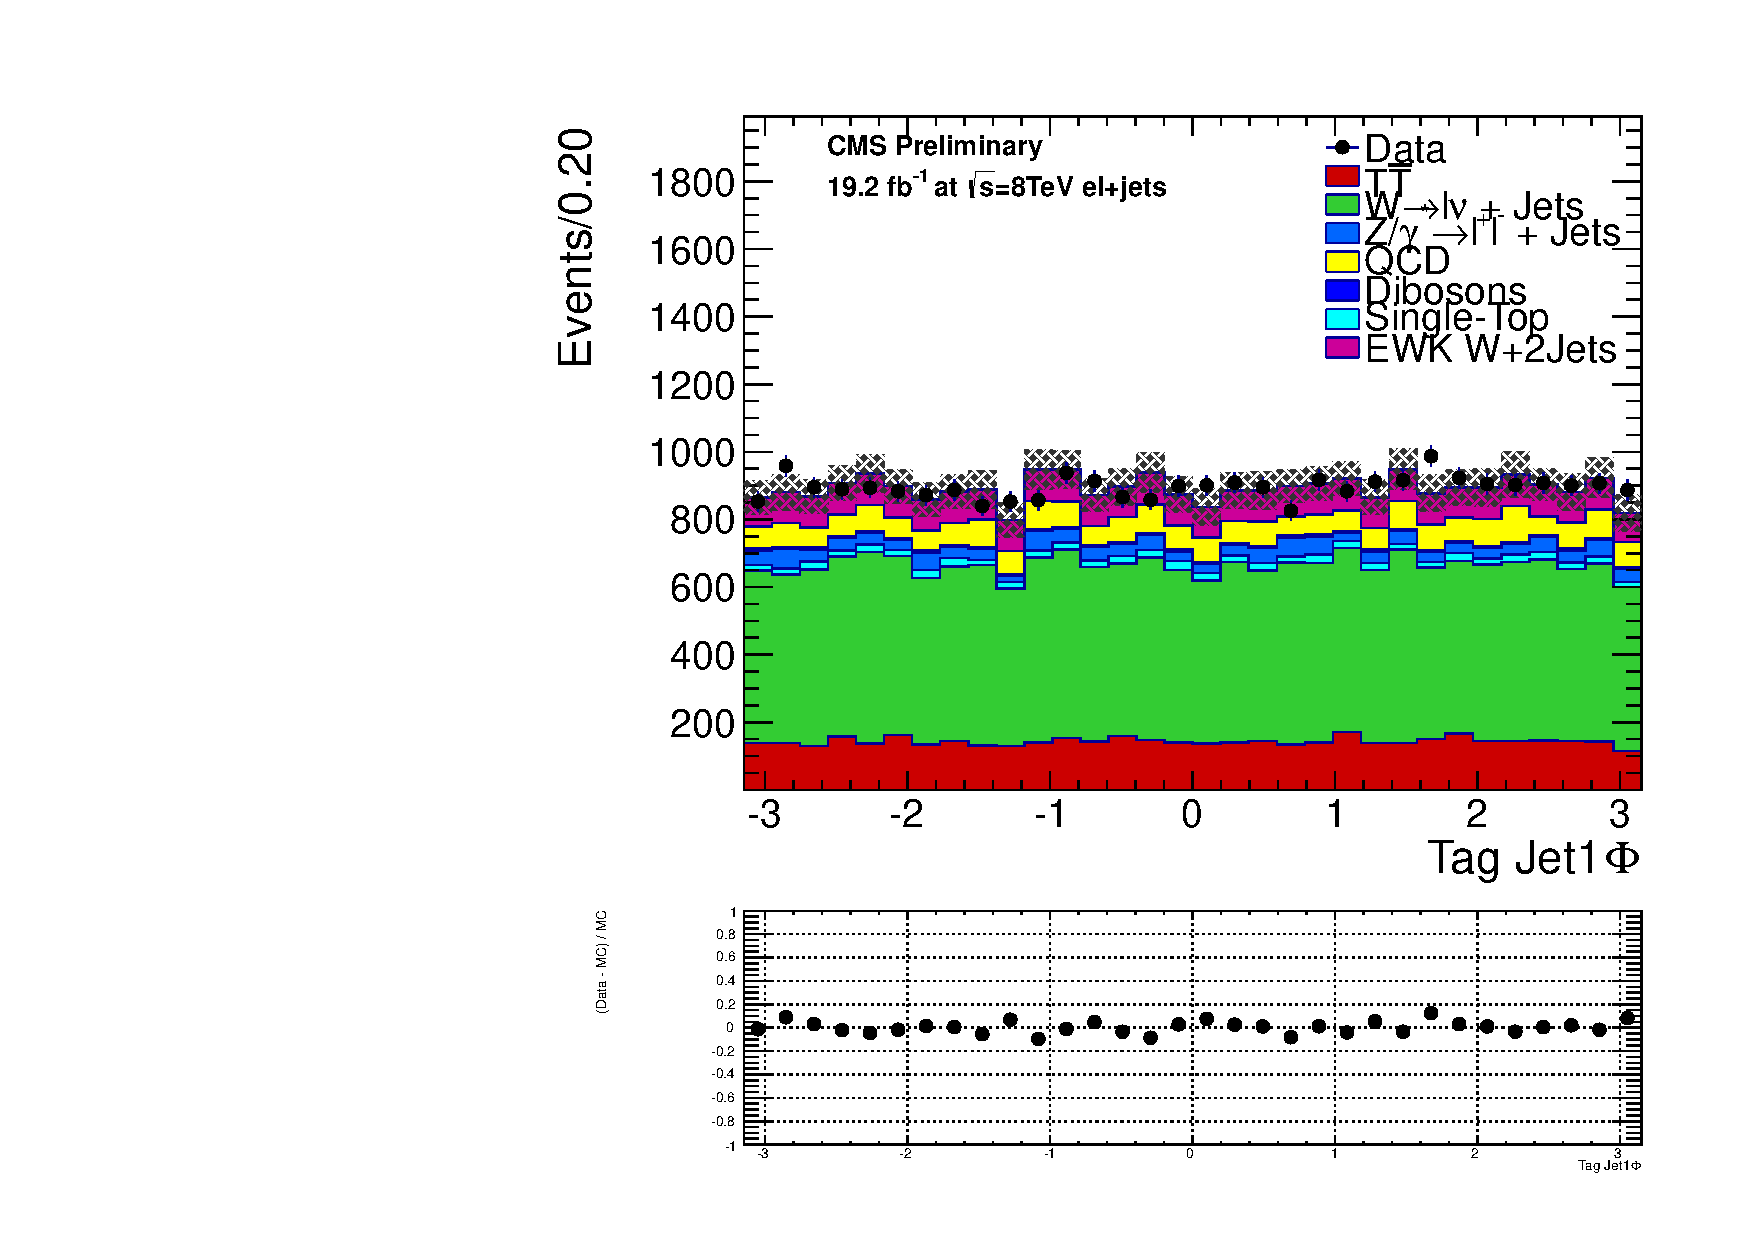
\includegraphics[width=0.49\textwidth]{figs/n-1_plots_el/el_EWK_W_2jets_tagjet1_phi_mjj_600_tagjet1_60_tagjet2_50_Zeppenfield_1point2_met_30_WmT_30_EWKW2jets.pdf}
    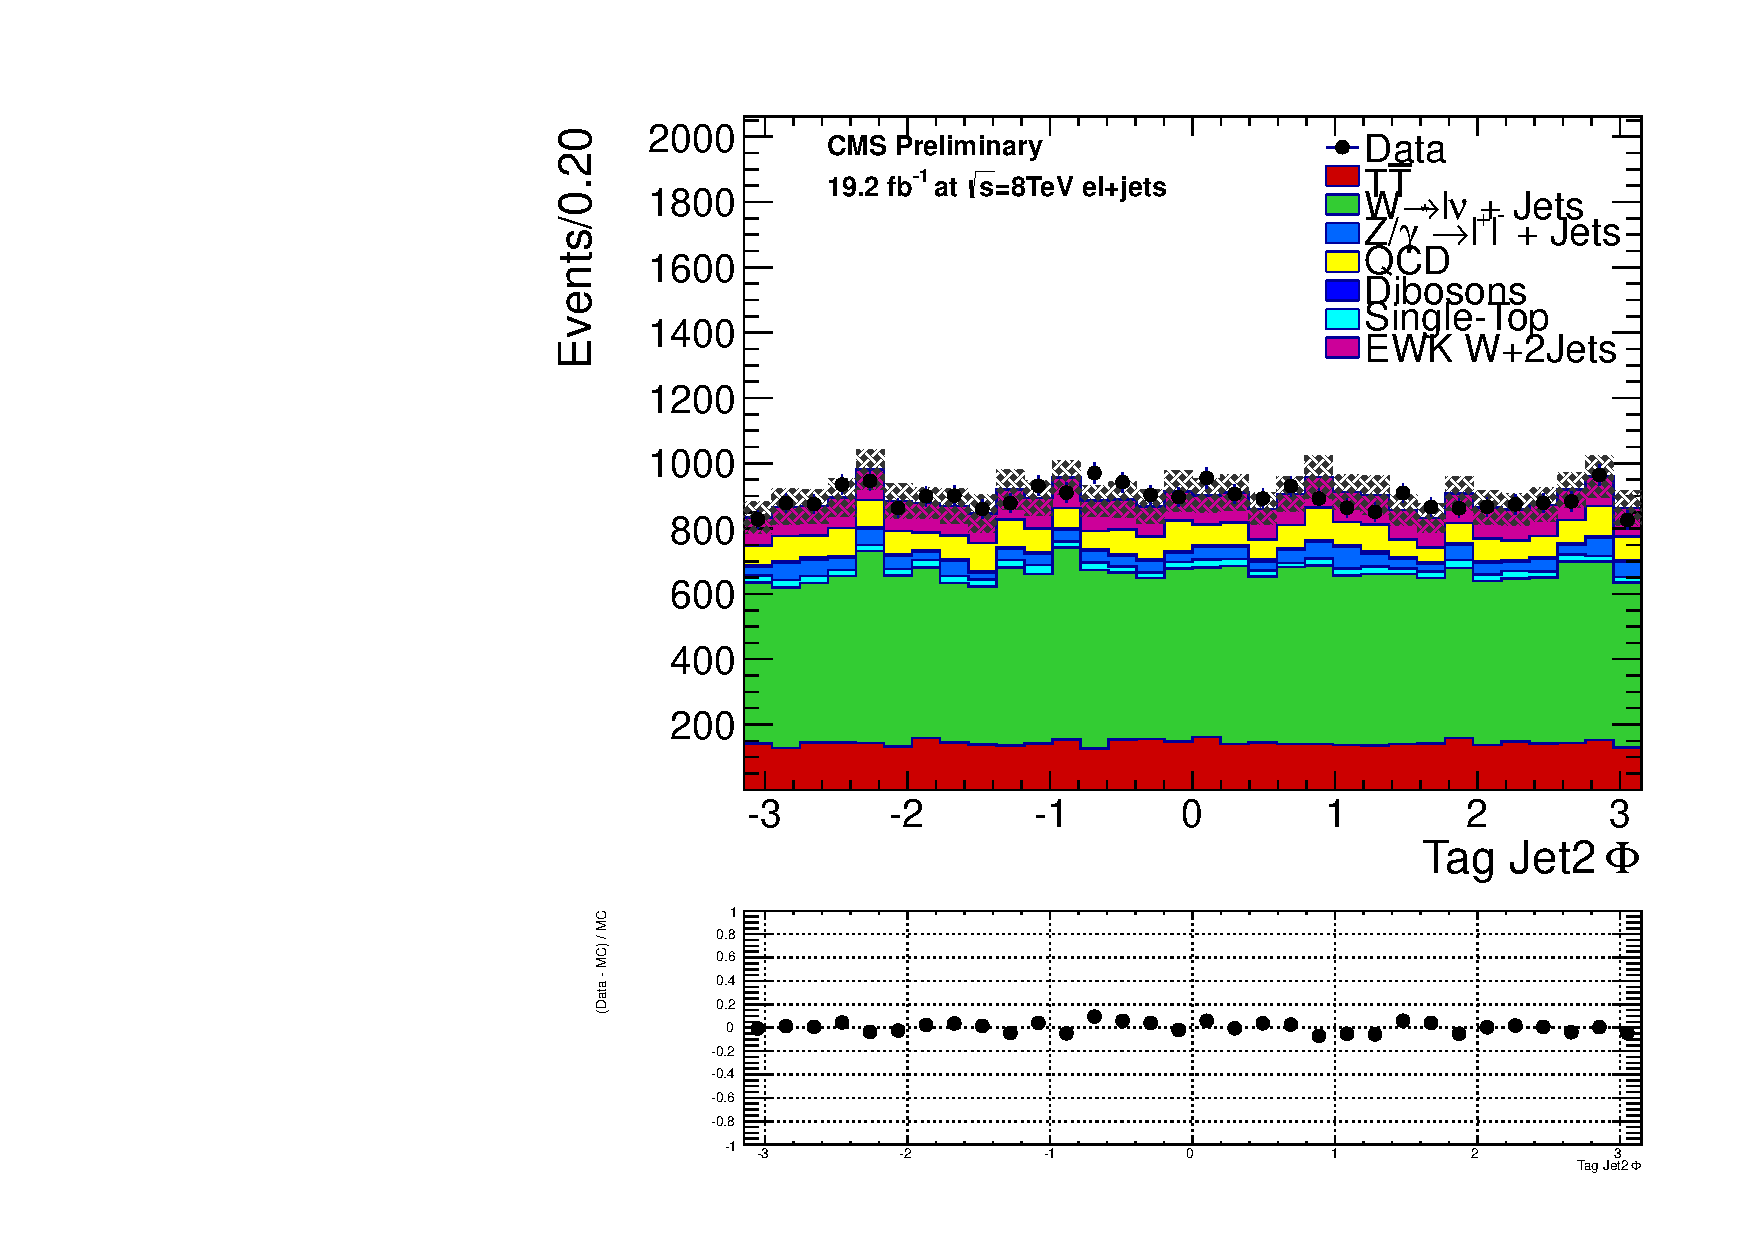
\includegraphics[width=0.49\textwidth]{figs/n-1_plots_el/el_EWK_W_2jets_tagjet2_phi_mjj_600_tagjet1_60_tagjet2_50_Zeppenfield_1point2_met_30_WmT_30_EWKW2jets.pdf}
    \caption{Comparison of the leading jet $\phi $ (left) and the
      second leading jet $\phi $ (right) distributions from data and MC for the electron+jets
      selection. 
      }
    \label{fig:elec_jet_phi}}
\end{figure}
%%%%%%%%%%%%%%%%%%%%%%%%%%%%
%%%%%%%%%%%%%%%%%%%%%%%%%%%%
\begin{figure}[h!t]
  {\centering
    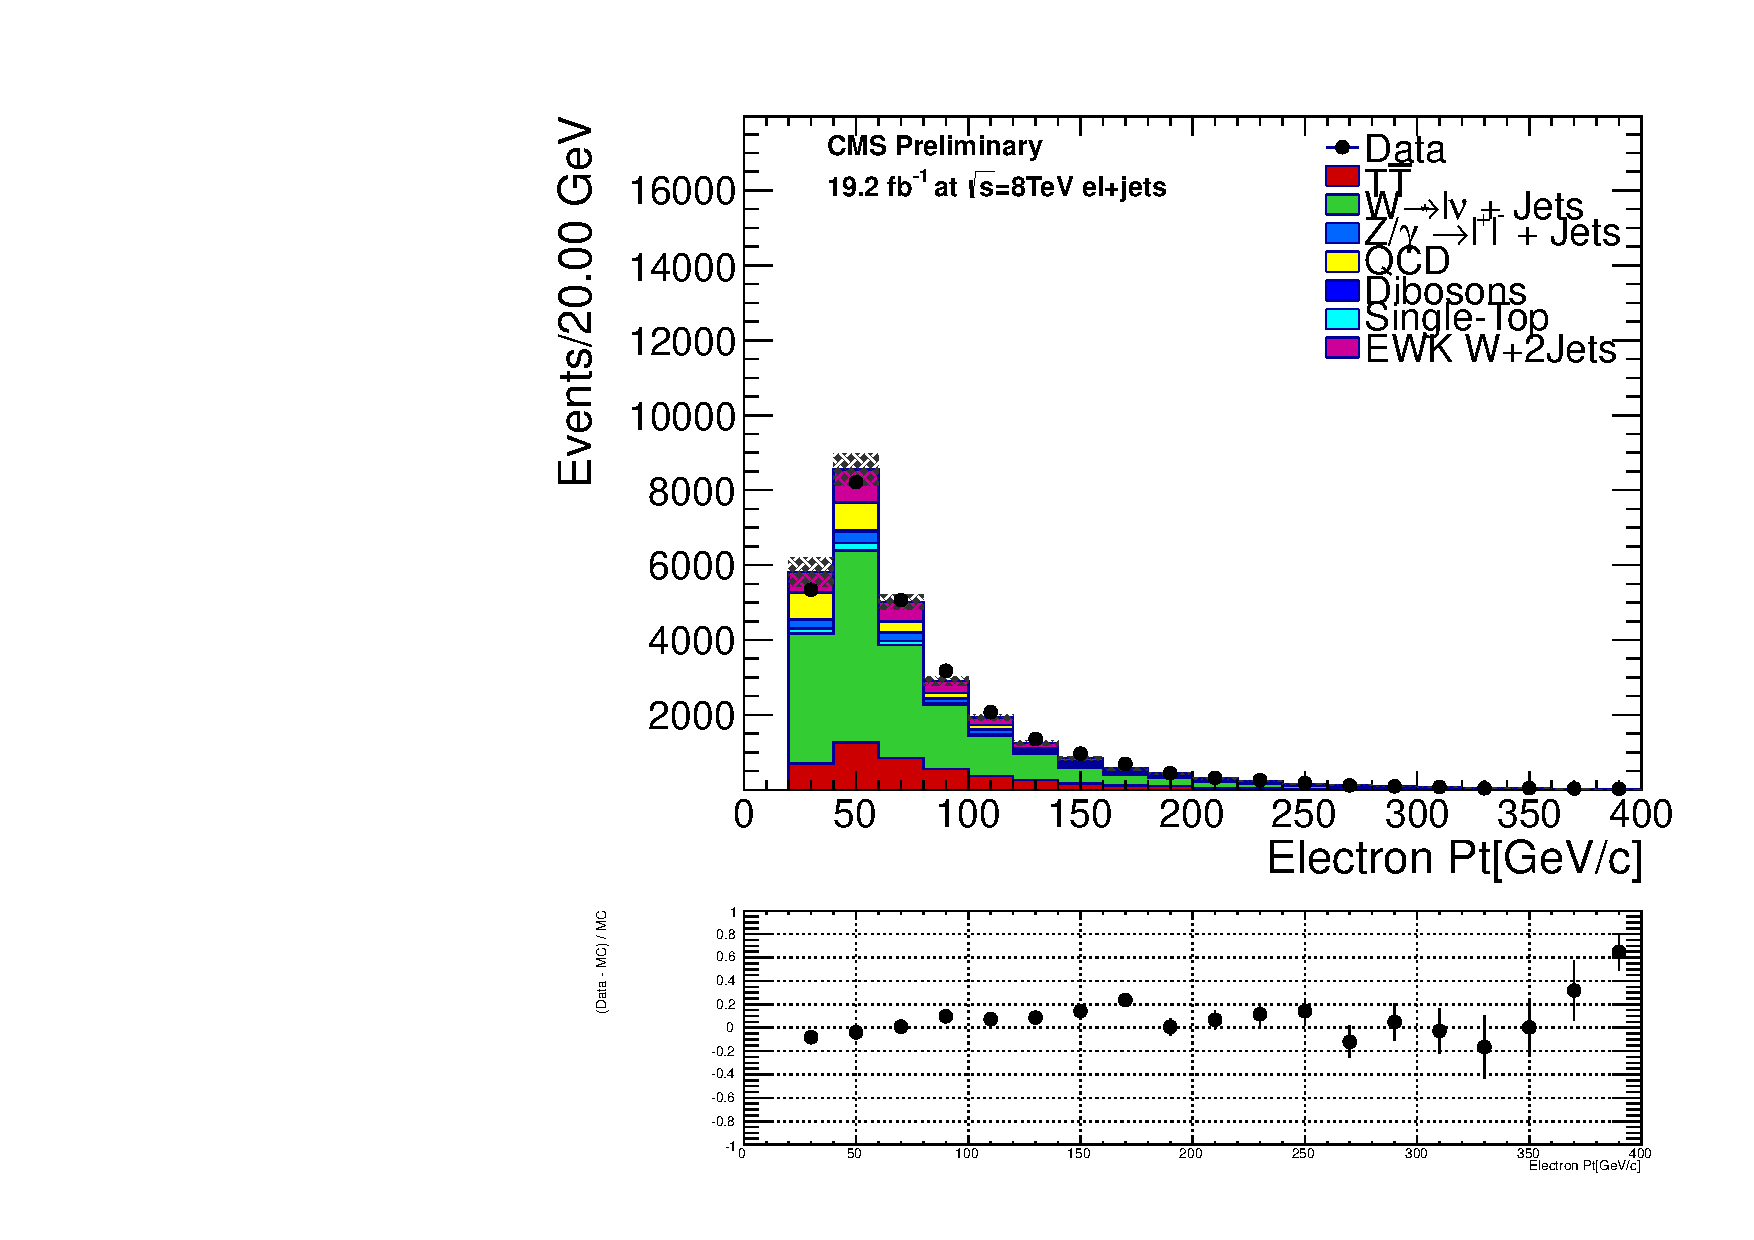
\includegraphics[width=0.49\textwidth]{figs/n-1_plots_el/el_EWK_W_2jets_l_pt_mjj_600_tagjet1_60_tagjet2_50_Zeppenfield_1point2_met_30_WmT_30_EWKW2jets.pdf}
    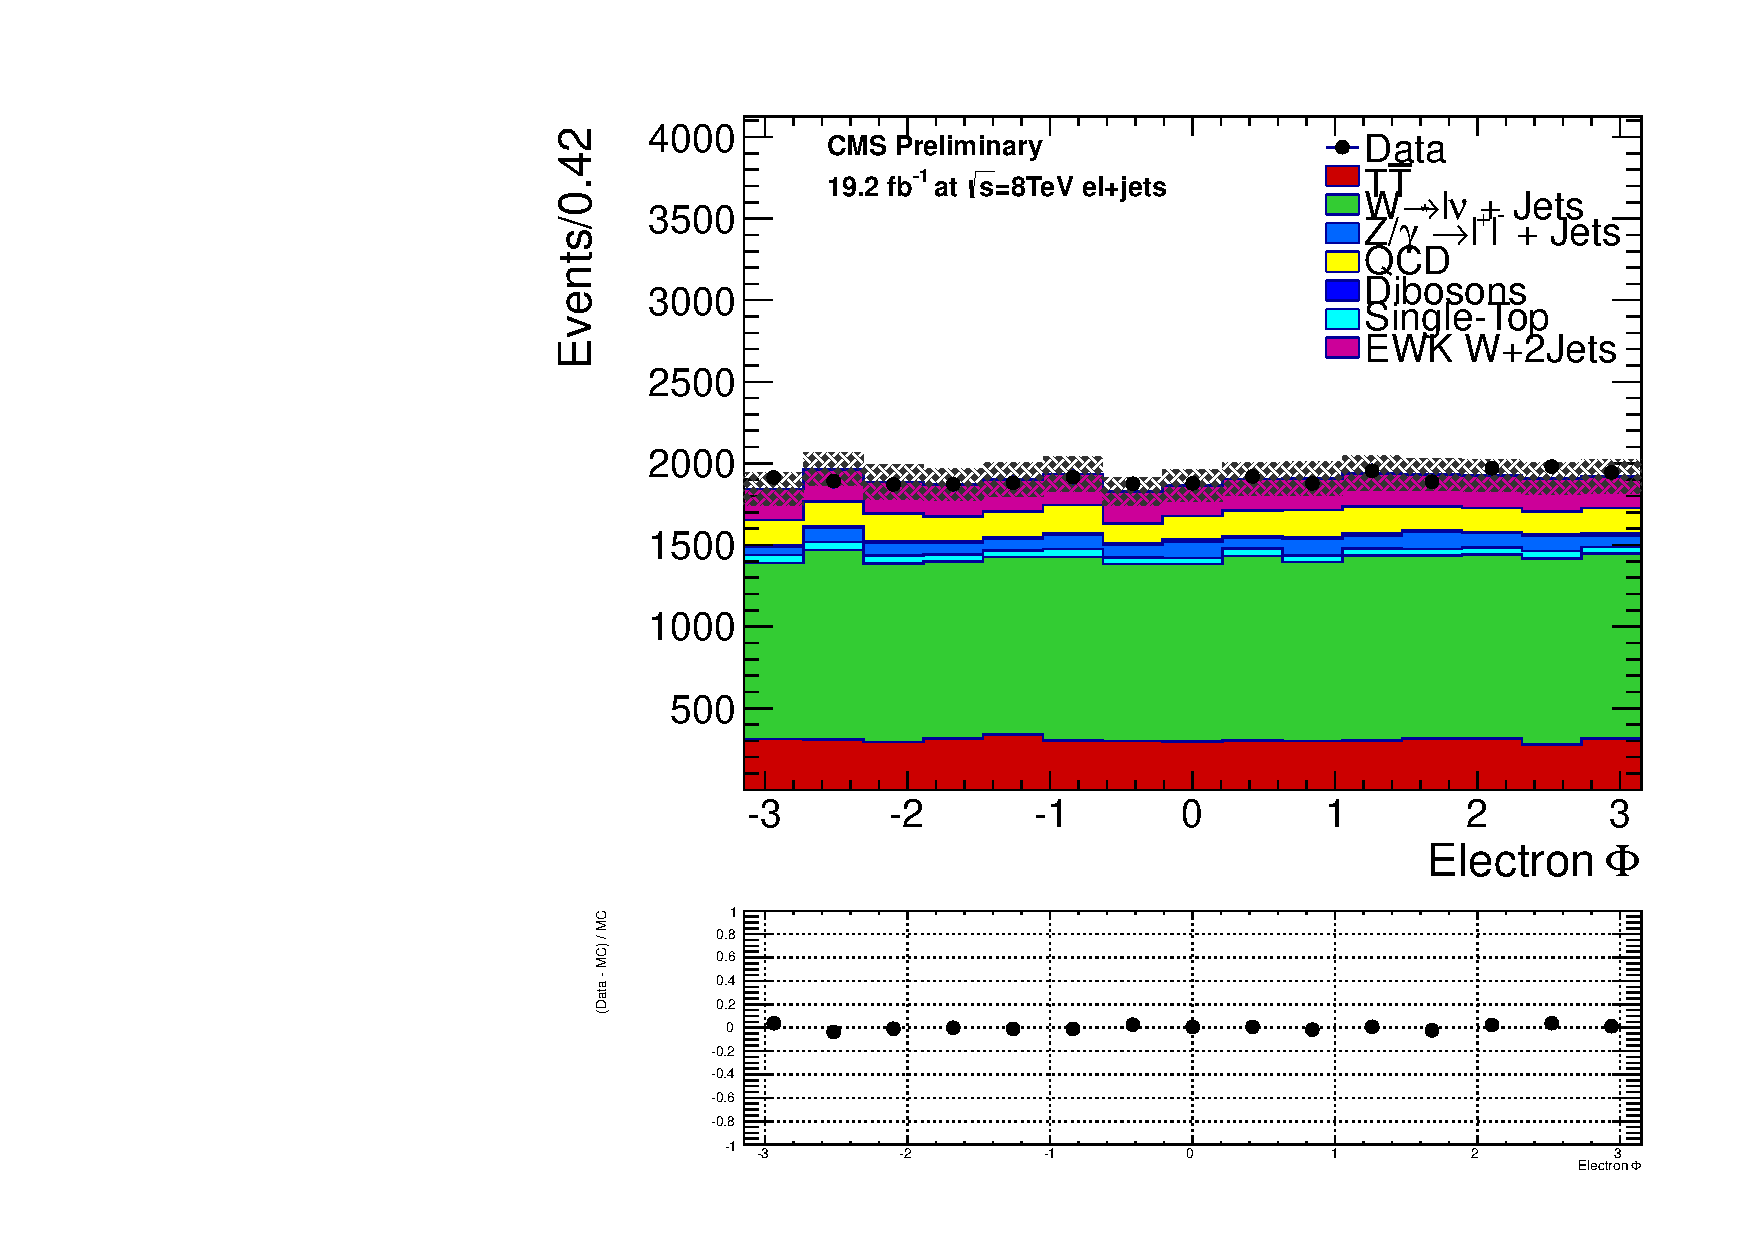
\includegraphics[width=0.49\textwidth]{figs/n-1_plots_el/el_EWK_W_2jets_l_phi_mjj_600_tagjet1_60_tagjet2_50_Zeppenfield_1point2_met_30_WmT_30_EWKW2jets.pdf}
    \caption{Comparison of the electron $E_{T} $ (left) and the
    electron $\phi $ (right) distributions from data and MC for the
    electron+jets selection. 
    }
   \label{fig:elec_electron}}
\end{figure}
%%%%%%%%%%%%%%%%%%%%%%%%%%%%
\begin{figure}[h!t]
  {\centering
    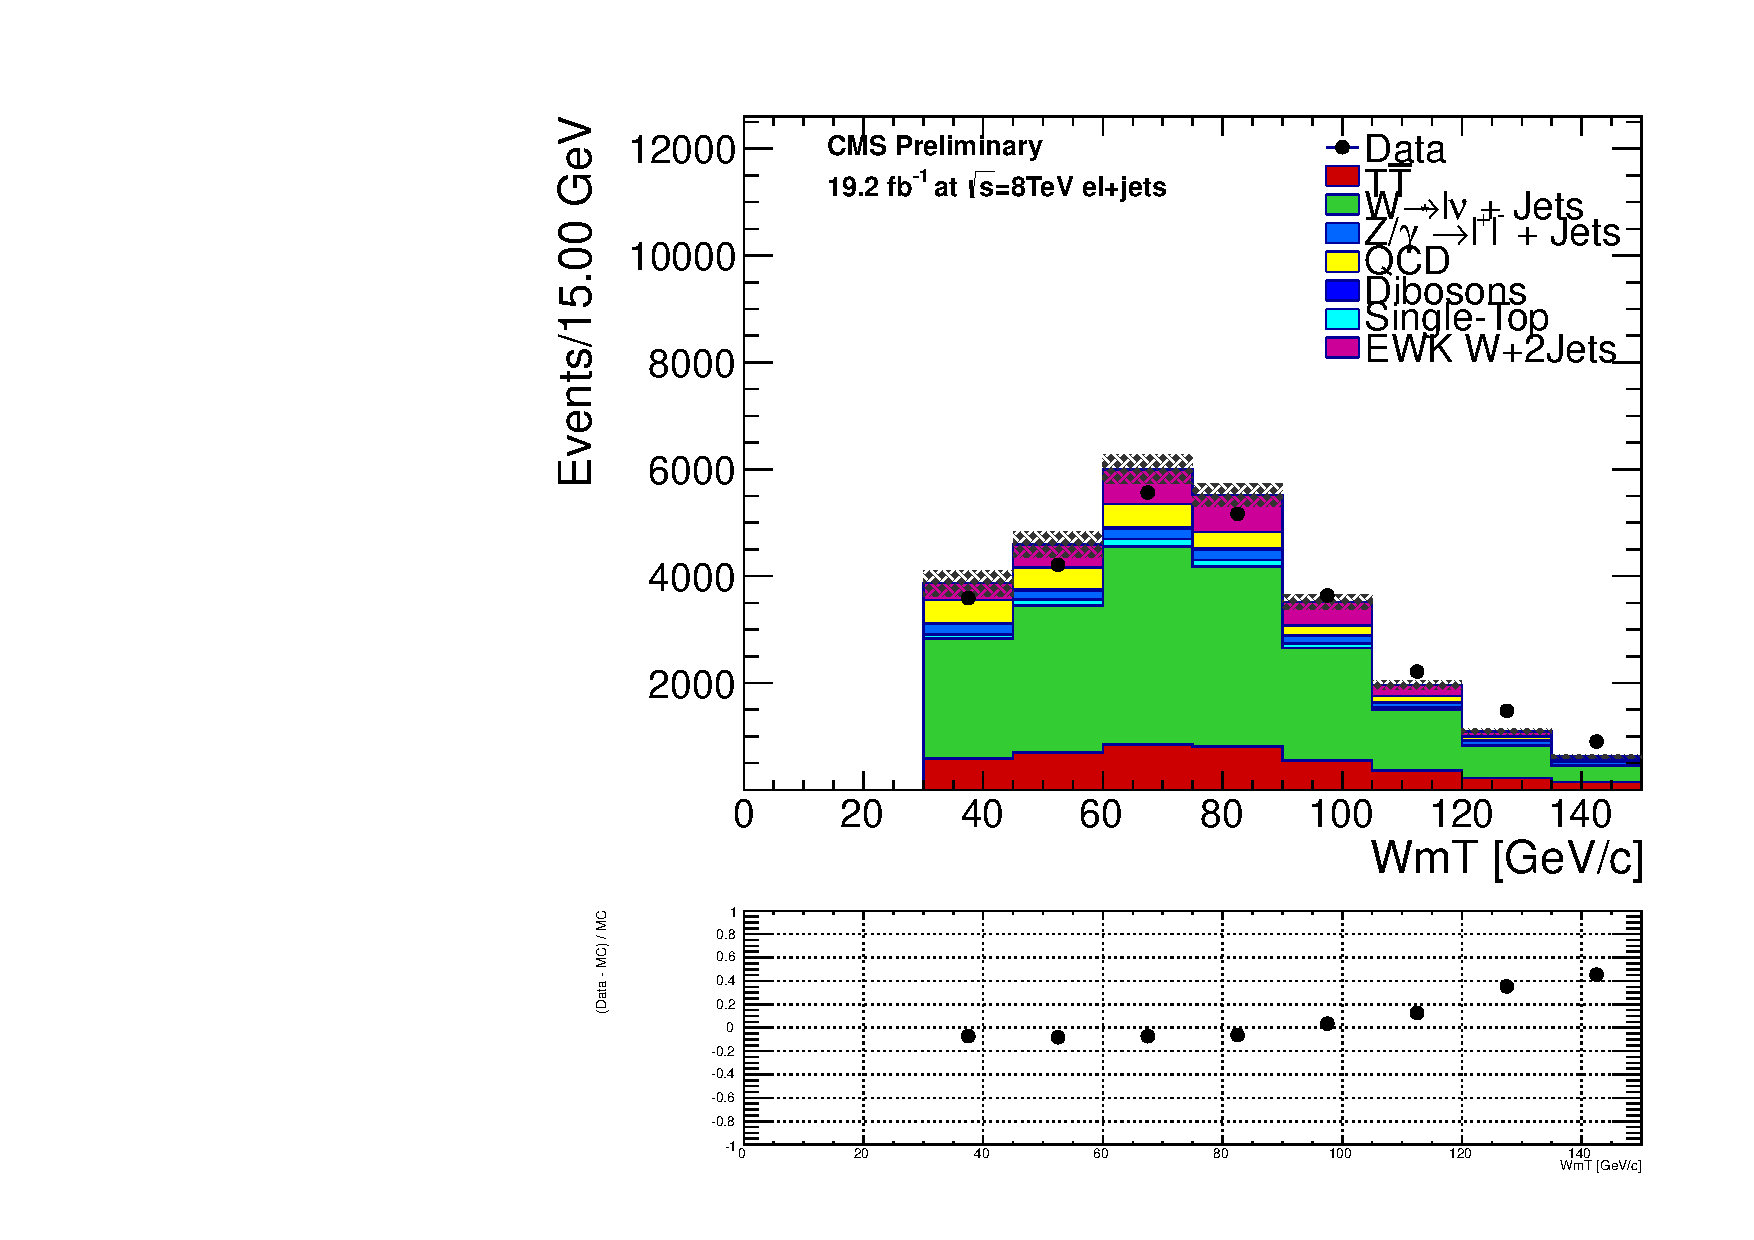
\includegraphics[width=0.49\textwidth]{figs/n-1_plots_el/el_EWK_W_2jets_W_mT_mjj_600_tagjet1_60_tagjet2_50_Zeppenfield_1point2_met_30_WmT_30_EWKW2jets.pdf}
    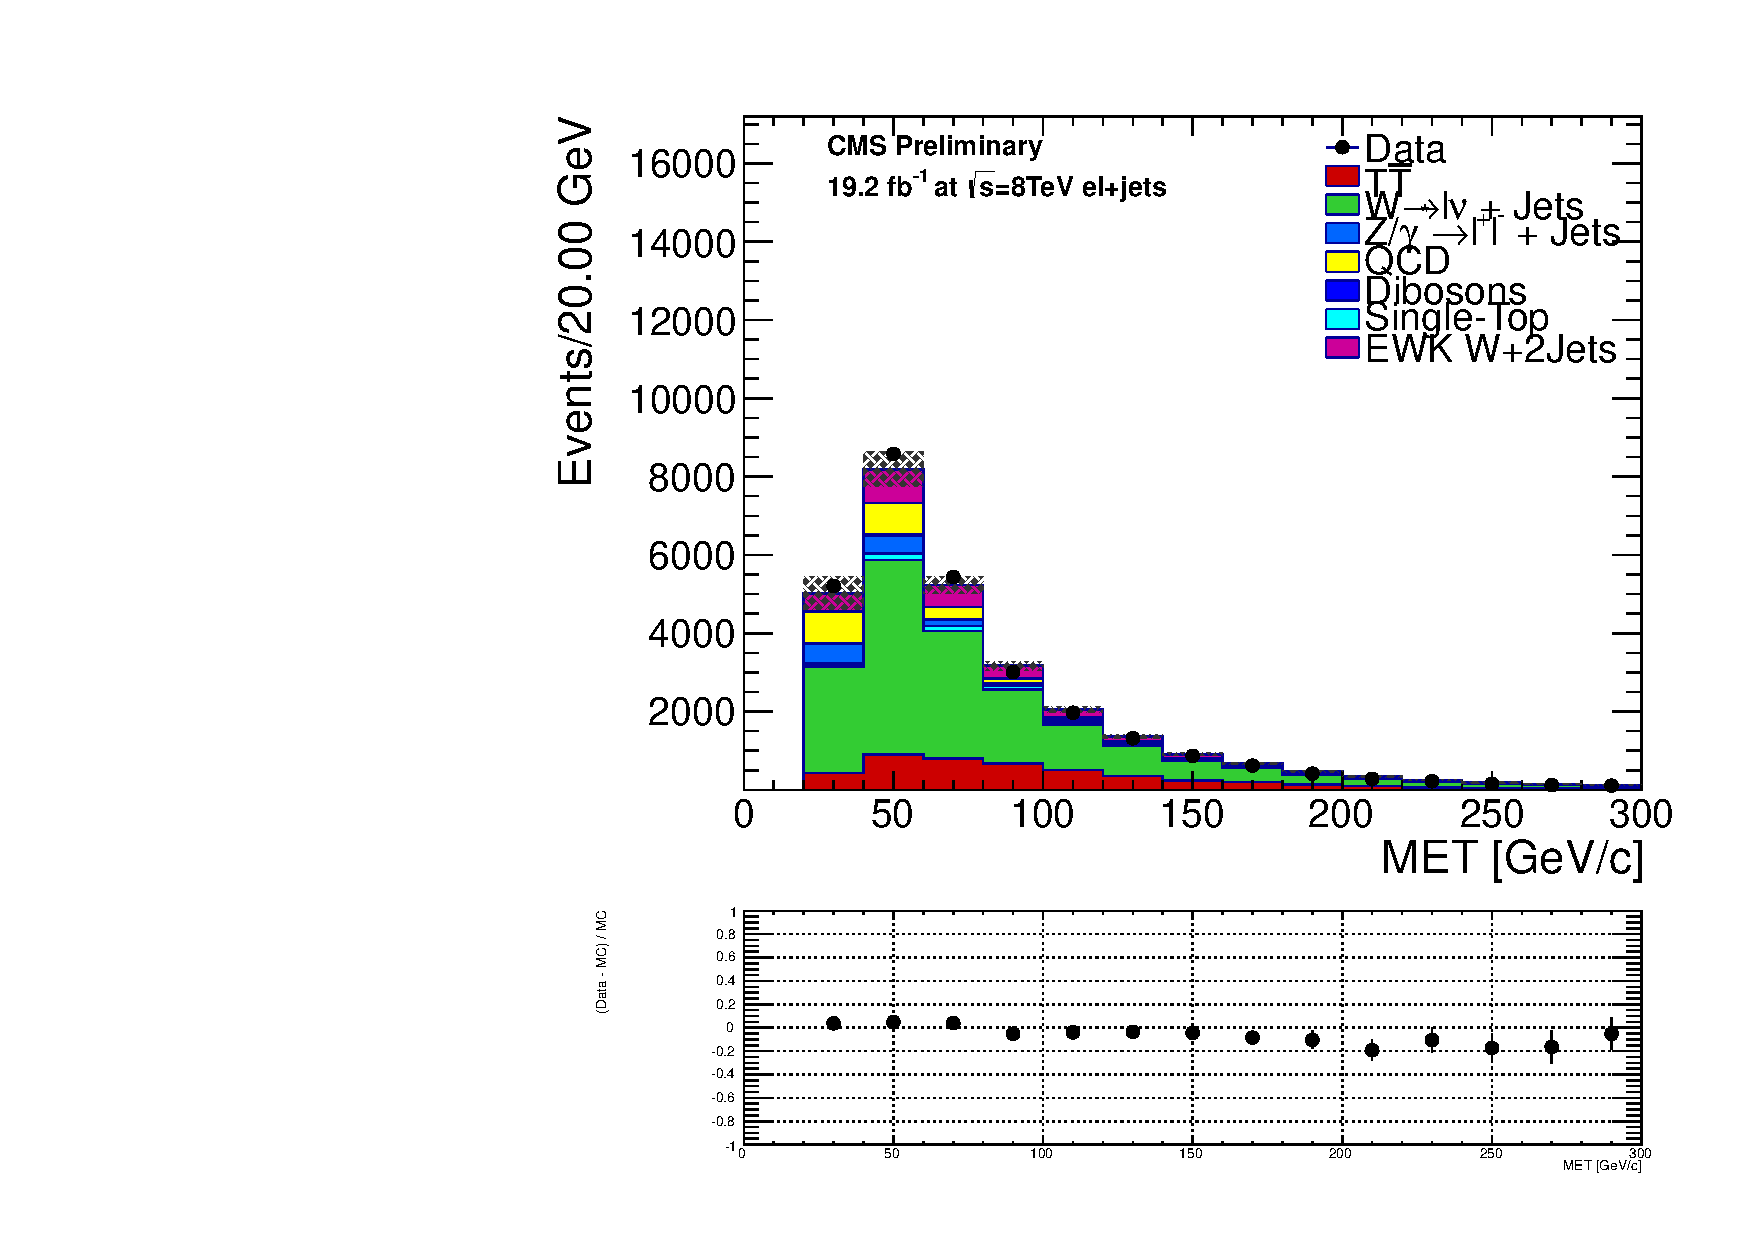
\includegraphics[width=0.49\textwidth]{figs/n-1_plots_el/el_event_met_pfmet_mjj_600_tagjet1_60_tagjet2_50_Zeppenfield_1point2_met_30_WmT_30_EWKW2jets.pdf}
    \caption{Comparison of the distributions from data and MC of the transverse mass
     of electron / MET system (left) and the MET (right) for the
      electron+jets selection. 
      }
    \label{fig:elec_W_Mt}}
\end{figure}
%%%%%%%%%%%%%%%%%%%%%%%%%%%%
\begin{figure}[h!t]
  {\centering
    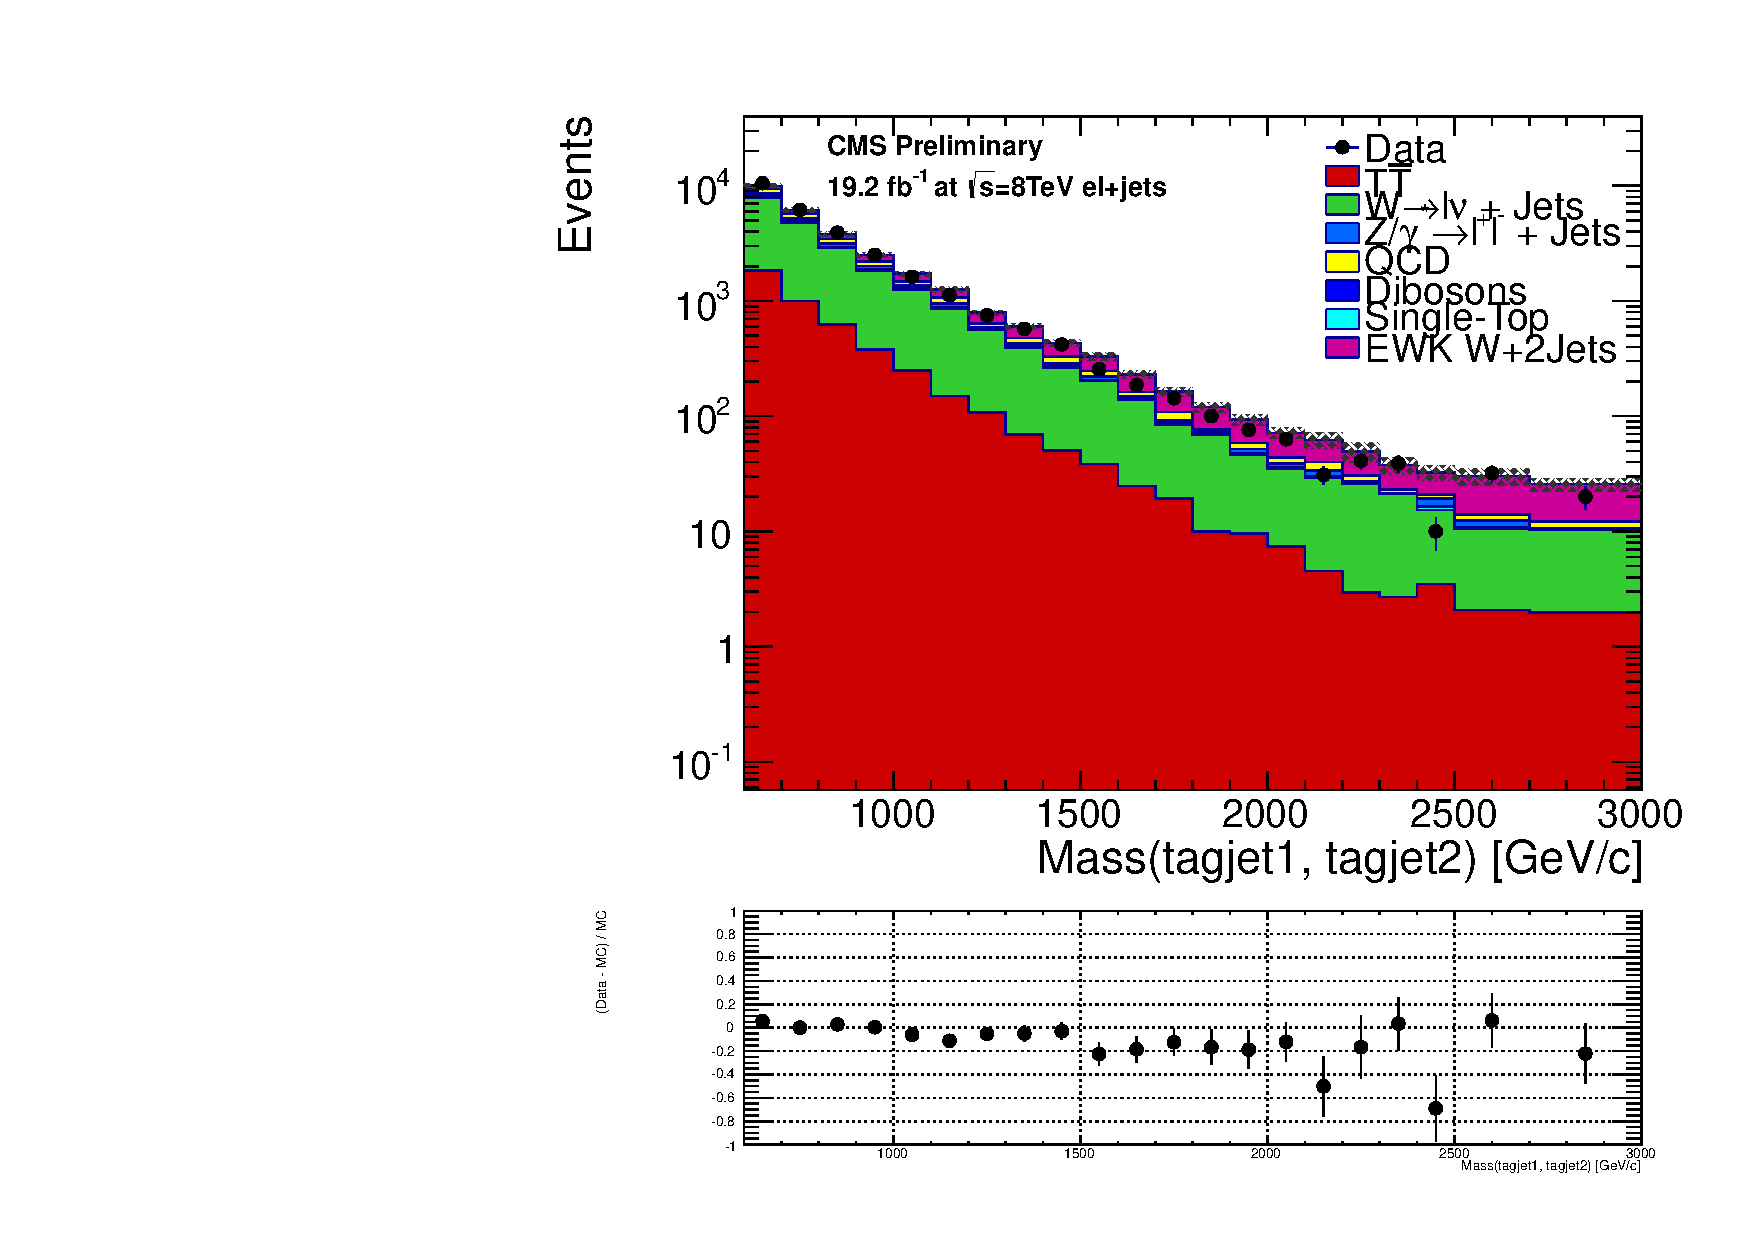
\includegraphics[width=0.49\textwidth]{figs/n-1_plots_el/el_EWK_W_2jets_tagjet_mass_mjj_600_tagjet1_60_tagjet2_50_Zeppenfield_1point2_met_30_WmT_30_logy_rebin_EWKW2jets.pdf}
    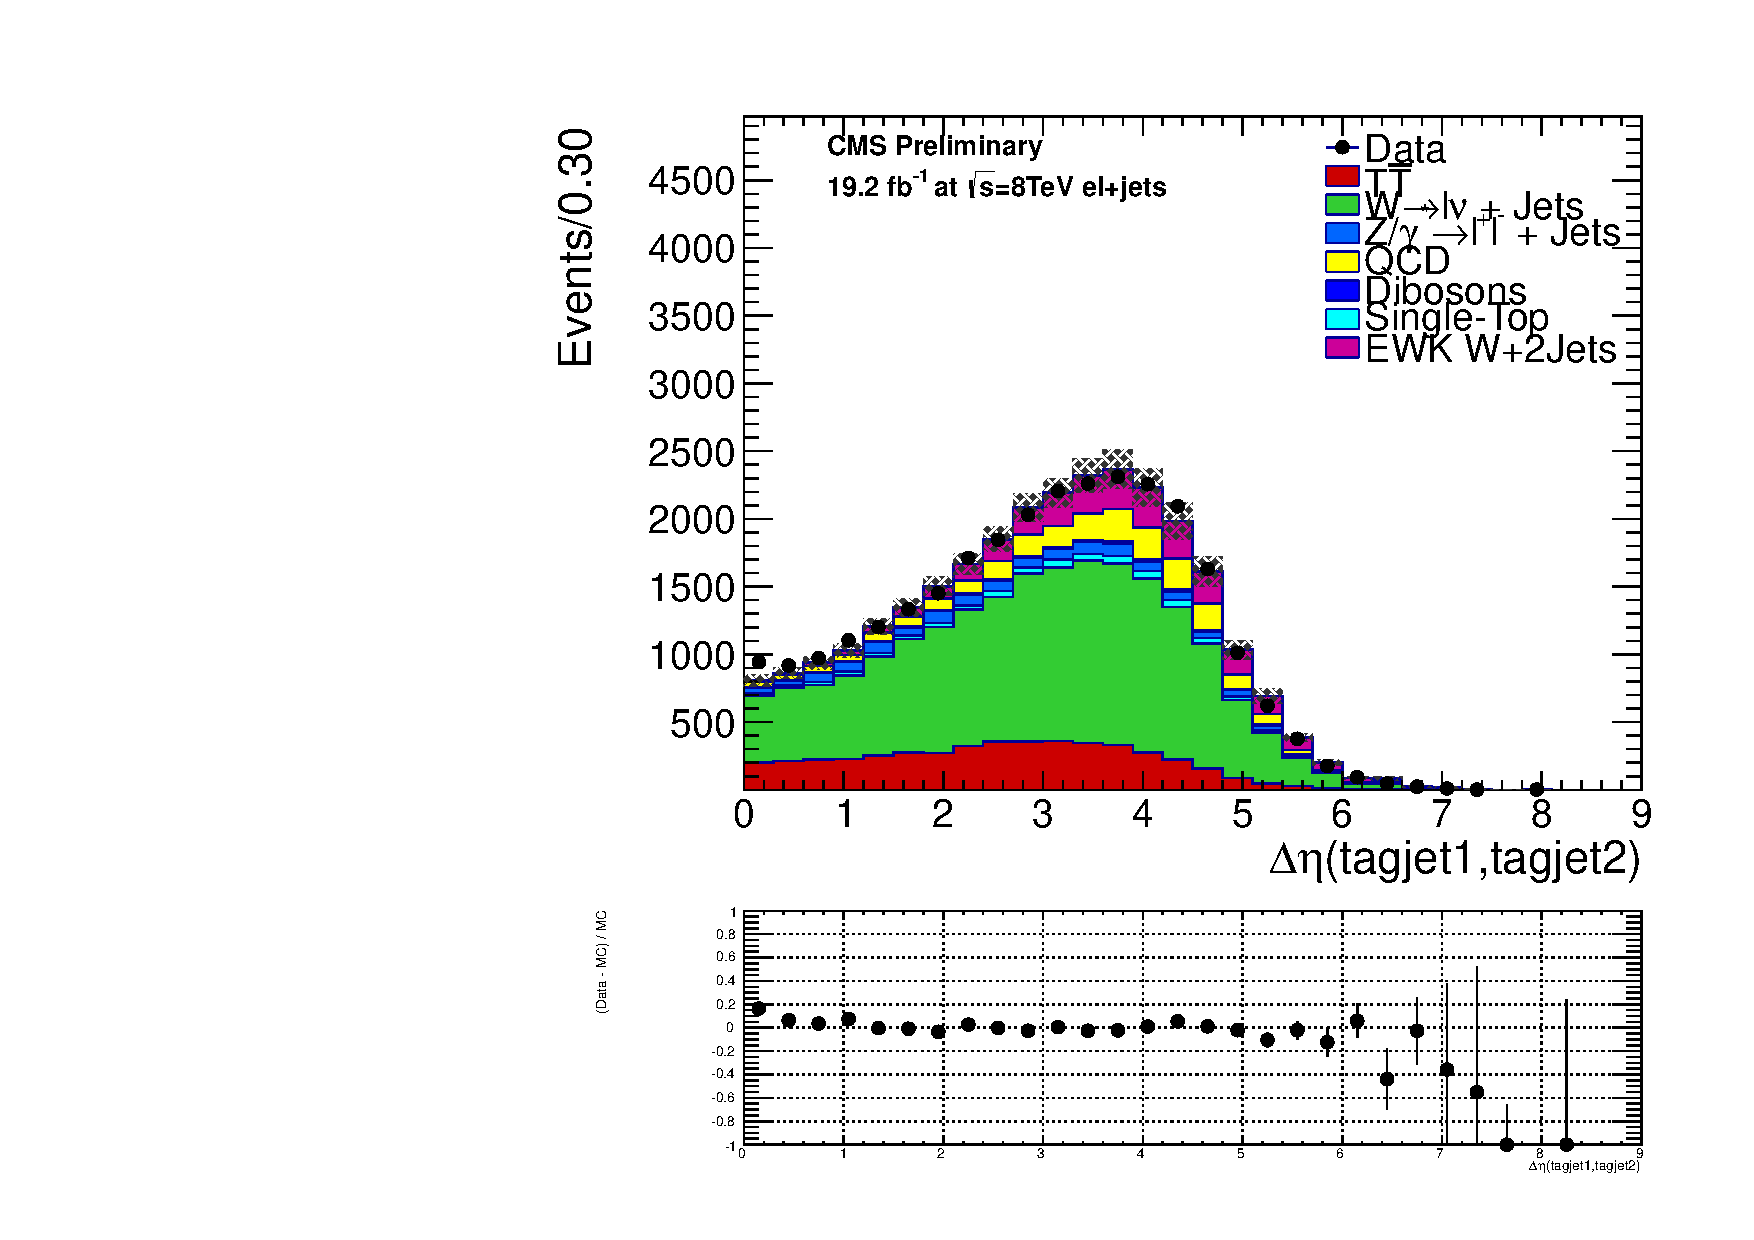
\includegraphics[width=0.49\textwidth]{figs/n-1_plots_el/el_EWK_W_2jets_tagjet_deltaeta_mjj_600_tagjet1_60_tagjet2_50_Zeppenfield_1point2_met_30_WmT_30_EWKW2jets.pdf}
    \caption{Comparison of the distributions from data and MC of the tag jet pair invariant mass (left)
      and the $\Delta\eta$ between the two tag jets (right) for the electron+jets selection. 
      }
    \label{fig:elec_dijet}}
\end{figure}
%%%%%%%%%%%%%%%%%%%%%%%%%%%%
\begin{figure}[ht]
\centerline{
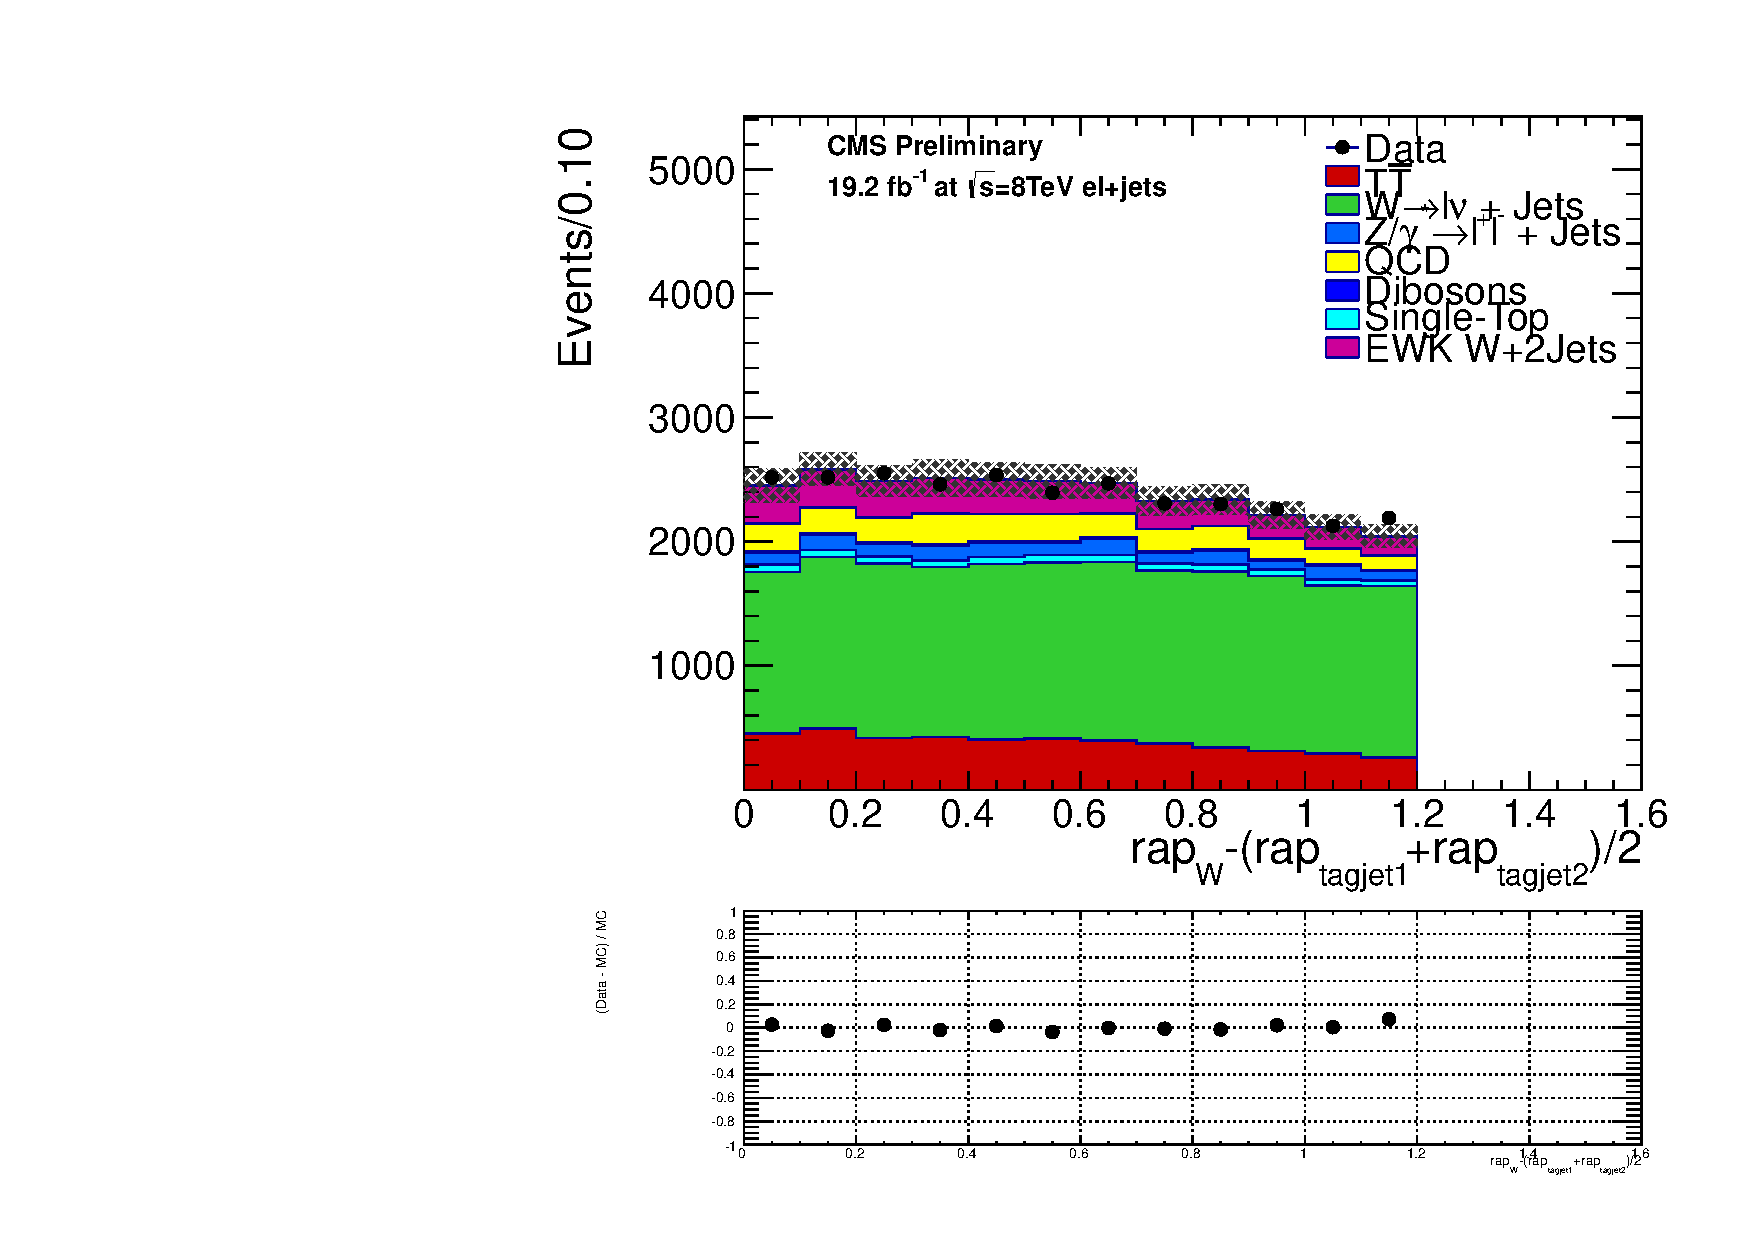
\includegraphics[width=.49\textwidth]{figs/n-1_plots_el/el_EWK_W_2jets_W_tagjet_Zeppenfield_mjj_600_tagjet1_60_tagjet2_50_Zeppenfield_1point2_met_30_WmT_30_EWKW2jets.pdf}
}
\caption{Comparison of the distributions from data and MC of the Zeppenfeld variable for electron+jets selection.}
\label{fig:elec_zeppenfield}
\end{figure}
%%%%%%%%%%%%%%%%%%%%%%%%%%%%
%\begin{figure}[htbp]
%\centering
%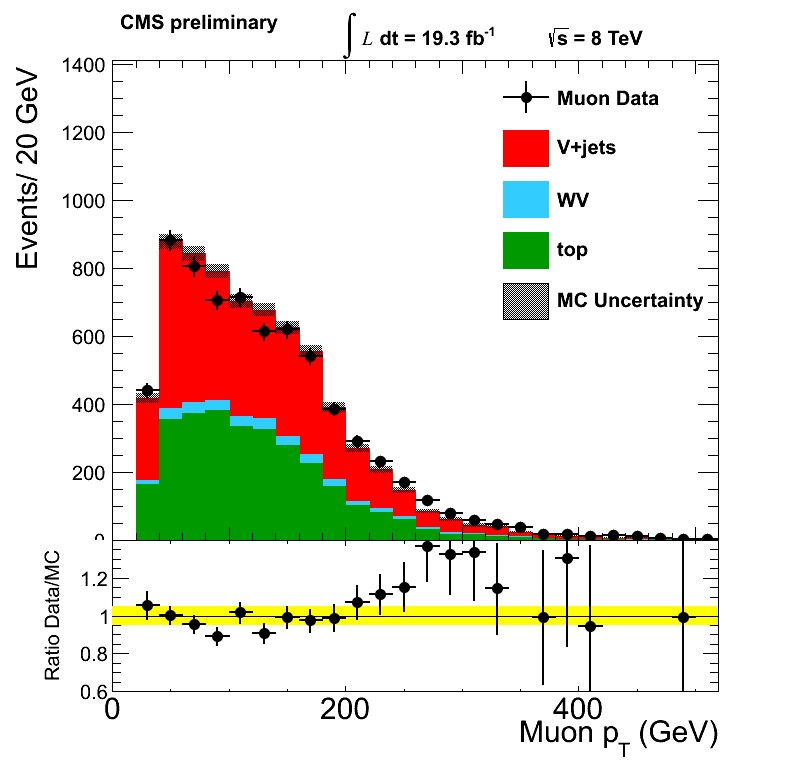
\includegraphics[width=0.45\textwidth]{figs/n-1_plots_mu/mu_W_muon_pt.png}
%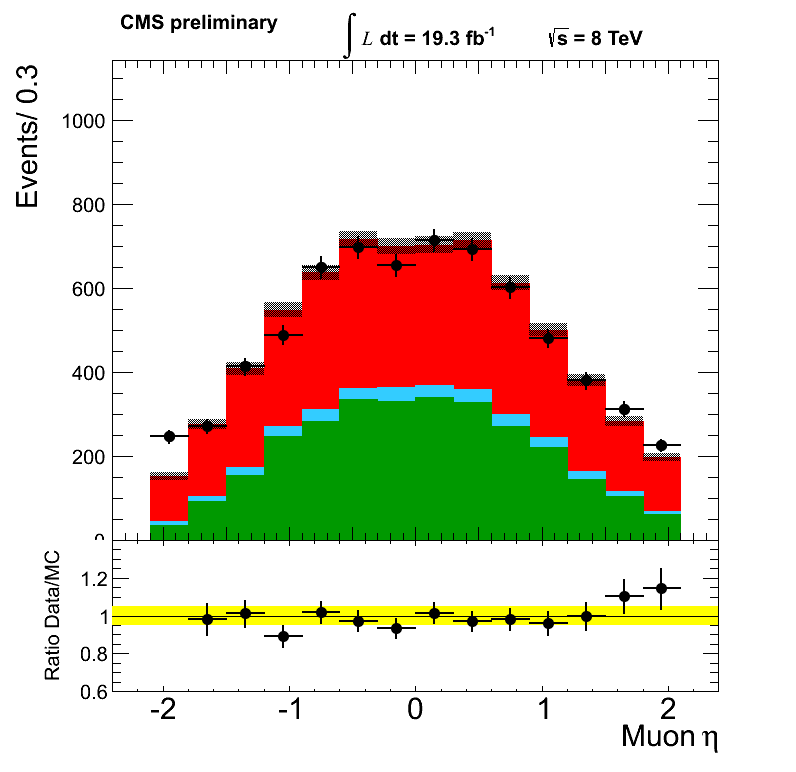
\includegraphics[width=0.45\textwidth]{figs/n-1_plots_mu/mu_W_muon_eta.png}
%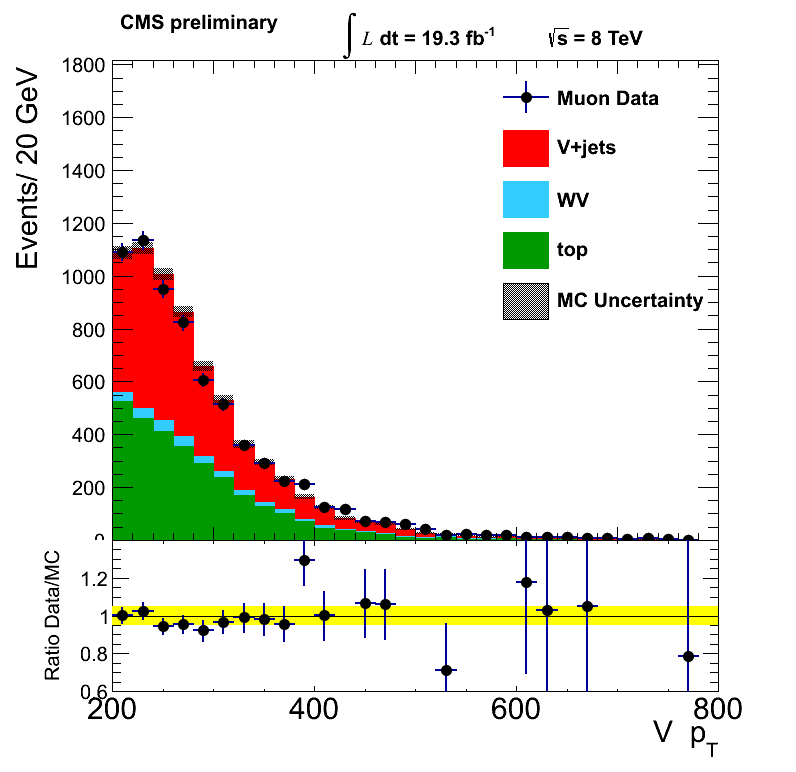
\includegraphics[width=0.45\textwidth]{figs/n-1_plots_mu/mu_W_pt.png}
%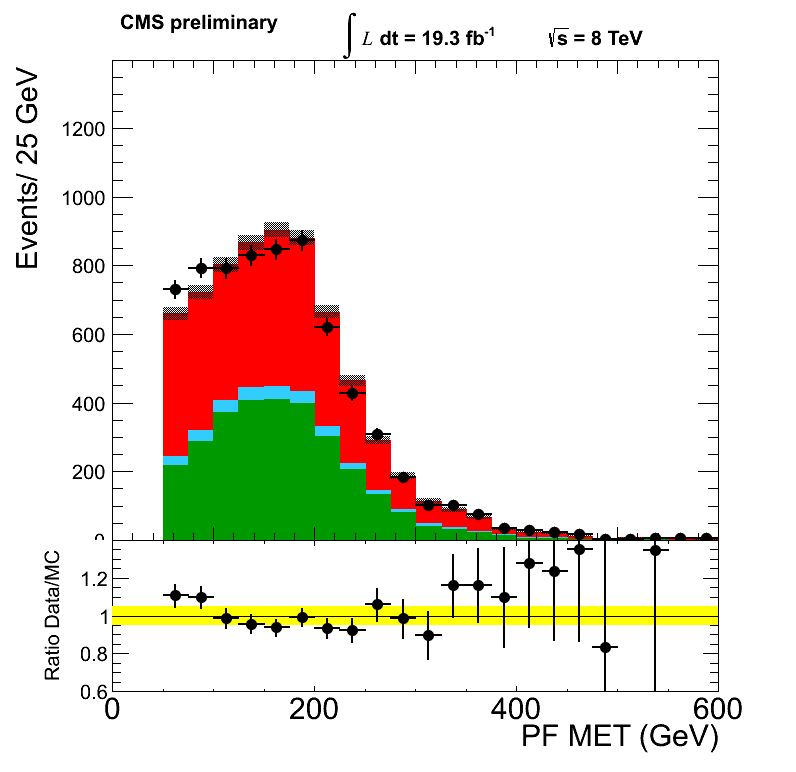
\includegraphics[width=0.45\textwidth]{figs/n-1_plots_mu/mu_event_met_pfmet.png}\\
%\caption{Boosted configuration control plots for muon channel: muon pT and $\eta$, W pT and MVA MET.}
%\label{fig:control_boosted_mu}
%\end{figure}
%
%\begin{figure}[htbp]
%\centering
%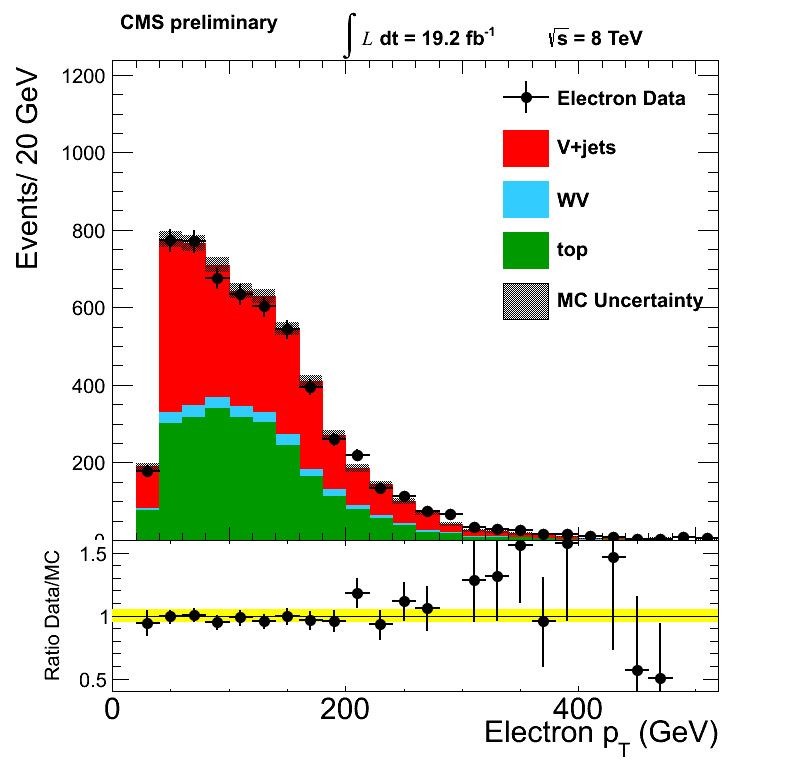
\includegraphics[width=0.45\textwidth]{figs/n-1_plots_el/el_W_elec_pt.png}
%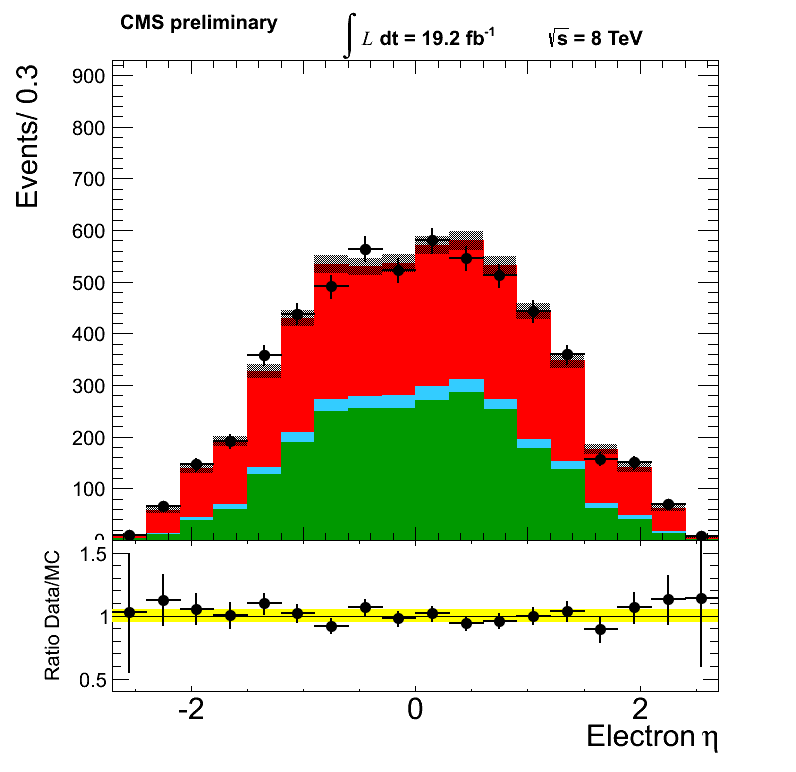
\includegraphics[width=0.45\textwidth]{figs/n-1_plots_el/el_W_elec_eta.png}\\
%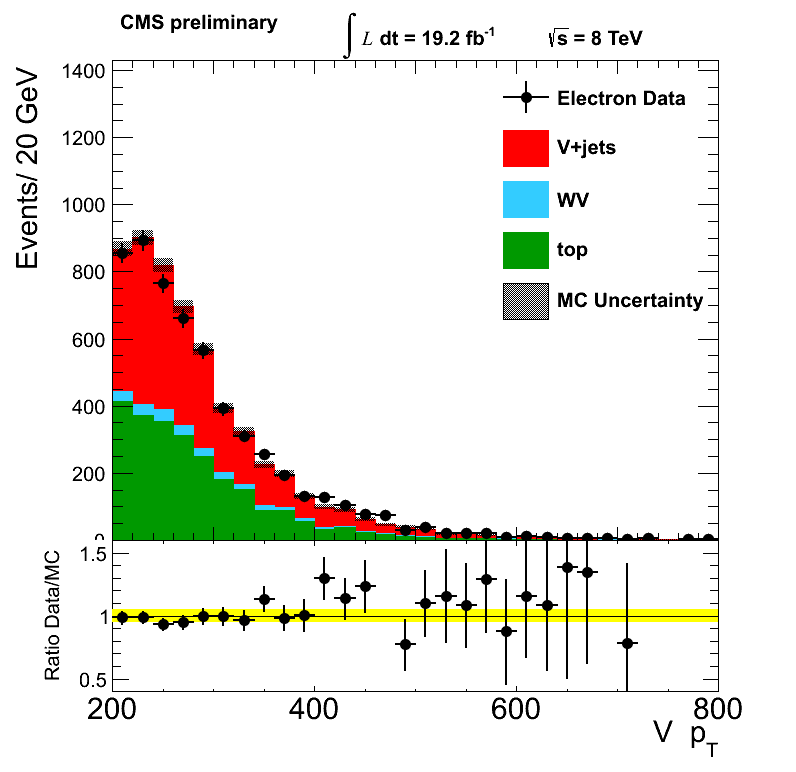
\includegraphics[width=0.45\textwidth]{figs/n-1_plots_el/el_W_pt.png}
%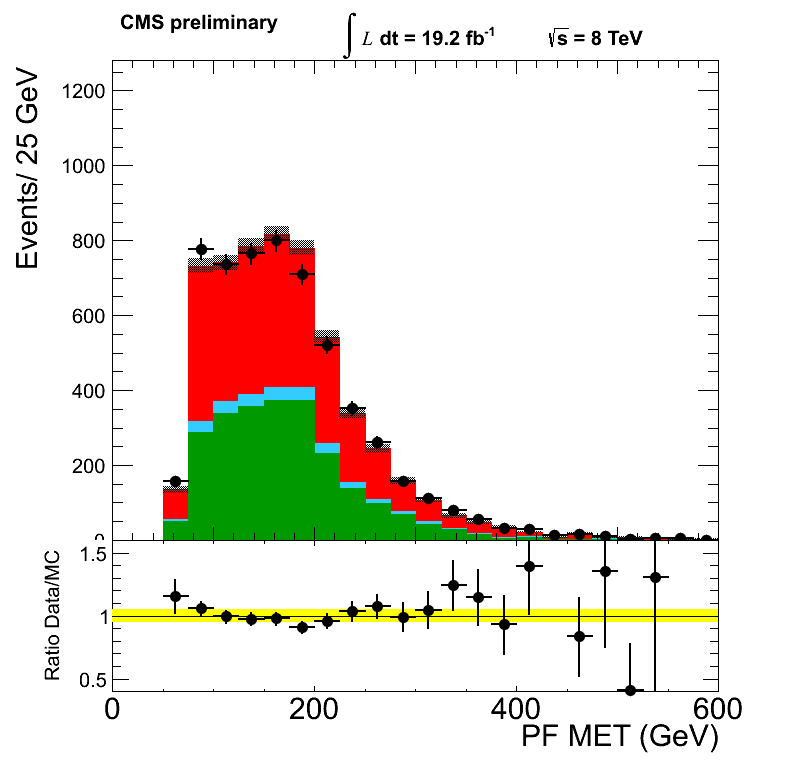
\includegraphics[width=0.45\textwidth]{figs/n-1_plots_el/el_event_met_pfmet.png}
%\caption{Boosted configuration control plots for electron channel: electron pT and $\eta$, W pT and MVA MET.}
%\label{fig:control_boosted_el}
%\end{figure}
%
%\begin{figure}[htbp]
%\centering
%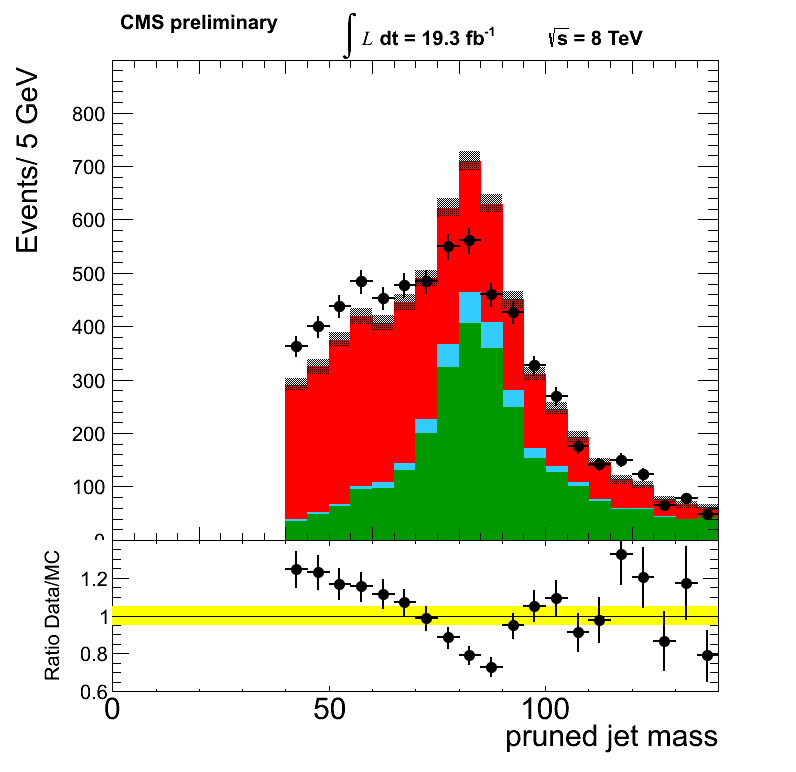
\includegraphics[width=0.45\textwidth]{figs/n-1_plots_mu/mu_GroomedJet_mass.png}
%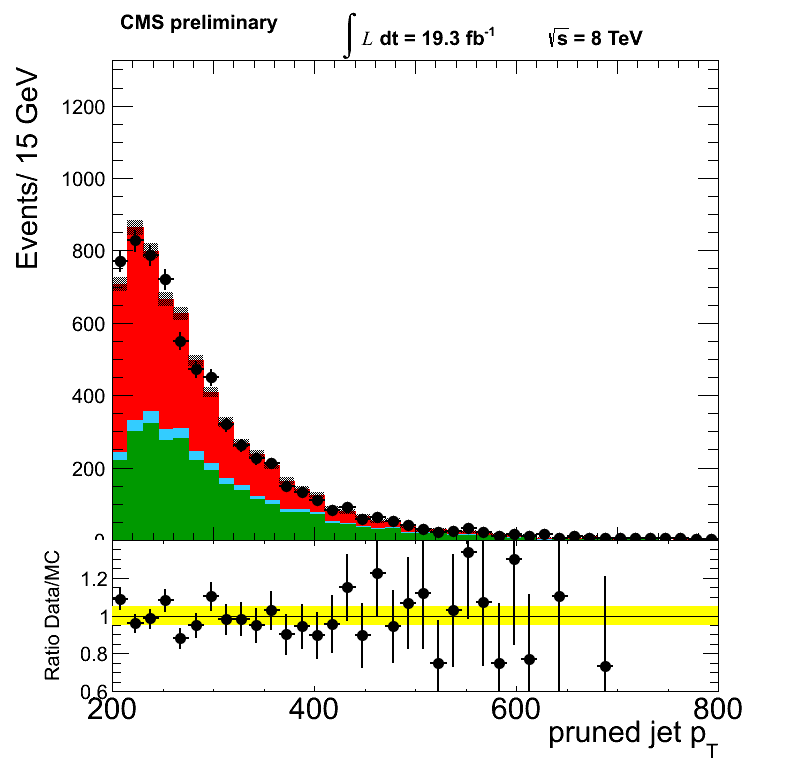
\includegraphics[width=0.45\textwidth]{figs/n-1_plots_mu/mu_GroomedJet_pt_pr.png}\\
%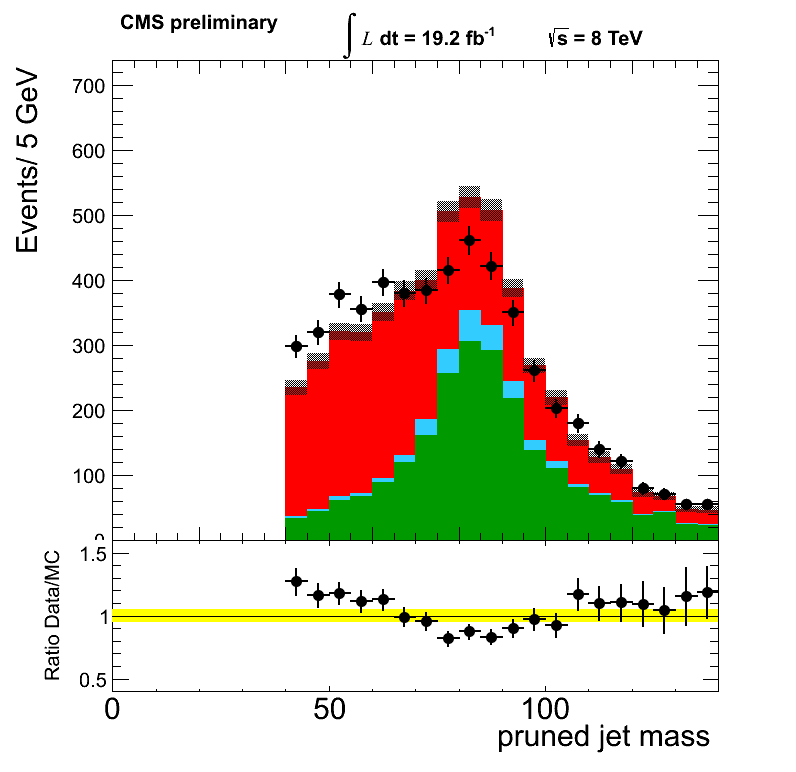
\includegraphics[width=0.45\textwidth]{figs/n-1_plots_el/el_GroomedJet_mass.png}
%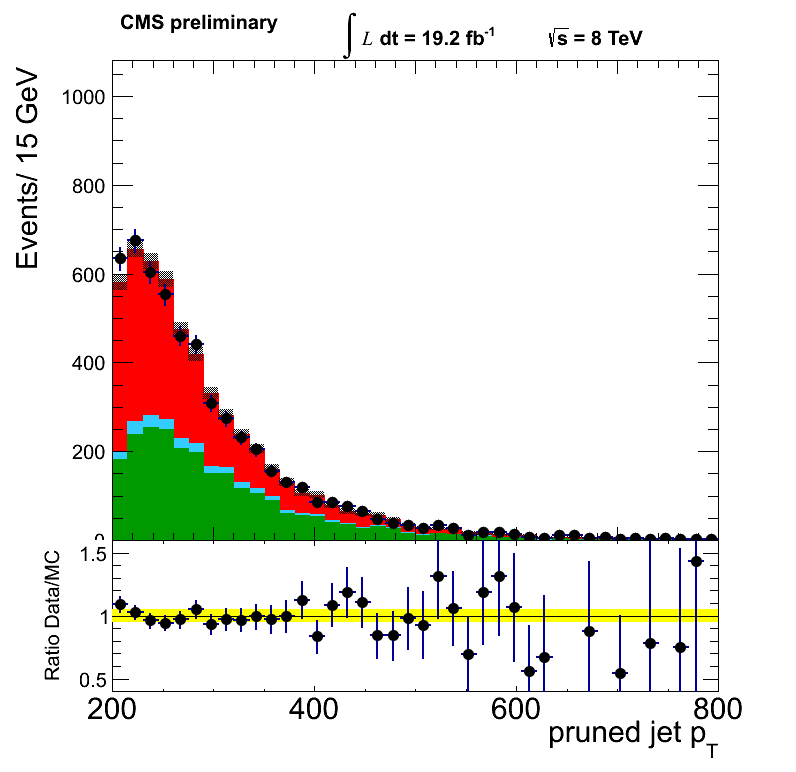
\includegraphics[width=0.45\textwidth]{figs/n-1_plots_el/el_GroomedJet_pt_pr.png}\\
%\caption{Boosted configuration control plots: pruned jet mass and pruned jet pT for muon (top) and electron (bottom) channels.}
%\label{fig:control_boosted_jet}
%\end{figure}
%%%%%%%%%%%%%%%%%%%%%%%%%%%%
%%%%%%%%%%%%%%%%%%%%%%%%%%%%
%%%%%%%%%%%%%%%%%%%%%%%%%%%%

\clearpage
%%%%%%%%%%%%%%%%%%%%%%%%%%%%%%%%%%%%%%%%%%%%%%%%%%%%%%%%%%%%%%%%%%%%
%%%%%%%%%%%%%%%%%%%%%%%%%%%%%%%%%%%%%%%%%%%%%%%%%%%%%%%%%%%%%%%%%%%%
%%%%%%%%%%%%%%%%%%%%%%%%%%%%%%%%%%%%%%%%%%%%%%%%%%%%%%%%%%%%%%%%%%%%

\section{Lepton reconstruction, selection and trigger efficiencies}
\label{sec:Eff}

Since the lepton reconstruction, selection and trigger efficiencies can be slightly different between data and simulation,
correction factors have to be applied to the MC to account for these differences. The efficiencies are calculated using a Tag and Probe
technique exploiting Z boson decays to a pair of electrons or muons, respectively. One of the leptons is used as tag and has to pass a
tight selection, while the second one is used as probe if the tag-probe pair combines to the Z boson mass. The total lepton efficiency
can be factorized into three components:

\begin{equation}
\epsilon_{\textnormal{total}}=\epsilon_{\textnormal{Reco}}\cdot\epsilon_{\textnormal{Id}}\cdot\epsilon_{\textnormal{HLT}}
\end{equation}

The tag and probe method is nearly the same compared to the one already used in the 2011 data analysis for this Higgs search
(\cite{CMS-AN-12-029},\cite{CMS-AN-2012-021}). Therefore, only the most important information will be discussed.

\subsection{Electron efficiencies}\label{subsec:EffEle}
In the electron case, the reconstruction efficiency $\epsilon_{\textnormal{Reco}}$ characterizes the transition from a supercluster in the
electromagnetic calorimeter to a reconstructed Particle Flow electron. The ability of a reconstructed electron to pass the offline
selection consisting of several isolation and identification criteria is given by the identification efficiency $\epsilon_{\textnormal{Id}}$.
Finally, the selected electron has a certain probability to fire the high level trigger and the efficiency to fulfill the HLT requirements 
is parametrized as $\epsilon_{\textnormal{HLT}}$. In data, a single electron trigger is used at HLT level, while in MC the HLT requirements are dropped. \\
Since the HLT efficiency is MC is equal to $100\%$, the HLT efficiency measured on data is applied directly in the analysis of MC samples, 
while the other two efficiency components are calculated both for data and MC, so that a data/MC scale factor is applied in the other cases. \\
In general, since the efficiency depends both on $\pt$ and $\eta$ of the electron, the measurement is binned in $\pt$ as (30, 35, 40, 45, 50, 200)\GeVc 
and in $\eta$ as (-2.5, -1.5, 0.0, 1.5, 2.5) of the probe electron. The resulting efficiencies and scale factors are summarized in Table~\ref{tab:eleEff} and
shown in Figure~\ref{fig:eleEff}. 

\begin{table}[htb]
\centering 
\scalebox{0.70}{
  \begin{tabular}{|c|c|c|c|c|c|c|}
  \hline
  $p_{\textnormal{T,min}}$ & $p_{\textnormal{T,max}}$ & $\eta_{\textnormal{min}}$ & $\eta_{\textnormal{max}}$ & $\epsilon_{\textnormal{Reco,data}}$/$\epsilon_{\textnormal{Reco,mc}}$ & $\epsilon_{\textnormal{ID,data}}$/$\epsilon_{\textnormal{ID,mc}}$ & $\epsilon_{\textnormal{HLT,data}}$ \\
  $[\GeVc]$         & $[\GeVc]$         &                     &                     &                              &                           &                               \\
  \hline
  \hline
  30 & 35 & -2.5 & -1.5 & 1.000 $\pm$ 0.002 & 0.973 $\pm$ 0.004 & 0.639 $\pm$ 0.003 \\
  30 & 35 & -1.5 & 0 & 0.996 $\pm$ 0.001 & 0.981 $\pm$ 0.003 & 0.874 $\pm$ 0.001 \\
  30 & 35 & 0 & 1.5 & 0.996 $\pm$ 0.001 & 0.980 $\pm$ 0.003 & 0.874 $\pm$ 0.001 \\
  30 & 35 & 1.5 & 2.5 & 1.002 $\pm$ 0.001 & 0.999 $\pm$ 0.004 & 0.650 $\pm$ 0.003 \\
  35 & 40 & -2.5 & -1.5 & 1.001 $\pm$ 0.001 & 1.005 $\pm$ 0.003 & 0.686 $\pm$ 0.002 \\
  35 & 40 & -1.5 & 0 & 0.999 $\pm$ 0.001 & 0.978 $\pm$ 0.002 & 0.896 $\pm$ 0.001 \\
  35 & 40 & 0 & 1.5 & 0.998 $\pm$ 0.001 & 0.978 $\pm$ 0.002 & 0.891 $\pm$ 0.002 \\
  35 & 40 & 1.5 & 2.5 & 1.001 $\pm$ 0.001 & 1.003 $\pm$ 0.085 & 0.690 $\pm$ 0.002 \\
  40 & 45 & -2.5 & -1.5 & 1.001 $\pm$ 0.001 & 1.005 $\pm$ 0.003 & 0.708 $\pm$ 0.002 \\
  40 & 45 & -1.5 & 0 & 0.999 $\pm$ 0.001 & 0.985 $\pm$ 0.001 & 0.909 $\pm$ 0.001 \\
  40 & 45 & 0 & 1.5 & 0.999 $\pm$ 0.001 & 0.983 $\pm$ 0.001 & 0.906 $\pm$ 0.001 \\
  40 & 45 & 1.5 & 2.5 & 1.000 $\pm$ 0.001 & 1.014 $\pm$ 0.003 & 0.720 $\pm$ 0.002 \\
  45 & 50 & -2.5 & -1.5 & 1.001 $\pm$ 0.001 & 1.017 $\pm$ 0.003 & 0.724 $\pm$ 0.002 \\
  45 & 50 & -1.5 & 0 & 1.000 $\pm$ 0.001 & 0.984 $\pm$ 0.002 & 0.917 $\pm$ 0.001 \\
  45 & 50 & 0 & 1.5 & 0.999 $\pm$ 0.001 & 0.985 $\pm$ 0.002 & 0.911 $\pm$ 0.001 \\
  45 & 50 & 1.5 & 2.5 & 1.001 $\pm$ 0.001 & 1.021 $\pm$ 0.003 & 0.733 $\pm$ 0.002 \\
  50 & 200 & -2.5 & -1.5 & 0.999 $\pm$ 0.001 & 1.023 $\pm$ 0.003 & 0.733 $\pm$ 0.003 \\
  50 & 200 & -1.5 & 0 & 0.999 $\pm$ 0.001 & 0.990 $\pm$ 0.002 & 0.925 $\pm$ 0.001 \\
  50 & 200 & 0 & 1.5 & 0.999 $\pm$ 0.001 & 0.991 $\pm$ 0.003 & 0.920 $\pm$ 0.001 \\
  50 & 200 & 1.5 & 2.5 & 1.000 $\pm$ 0.001 & 1.019 $\pm$ 0.003 & 0.745 $\pm$ 0.003 \\
  \hline
  \end{tabular}}
\caption{Electron efficiency and data/MC scale factors for super-cluster to reconstructed electrons ($\epsilon_{\textnormal{Reco}}$),
    reconstructed to selected electrons ($\epsilon_{\textnormal{ID}}$) and selected to HLT electrons ($\epsilon_{\textnormal{HLT}}$). 
    The errors are statistical only.} 
\label{tab:eleEff} 
\end{table}

\begin{figure}[b]
  \begin{center}
    \subfigure[]{
    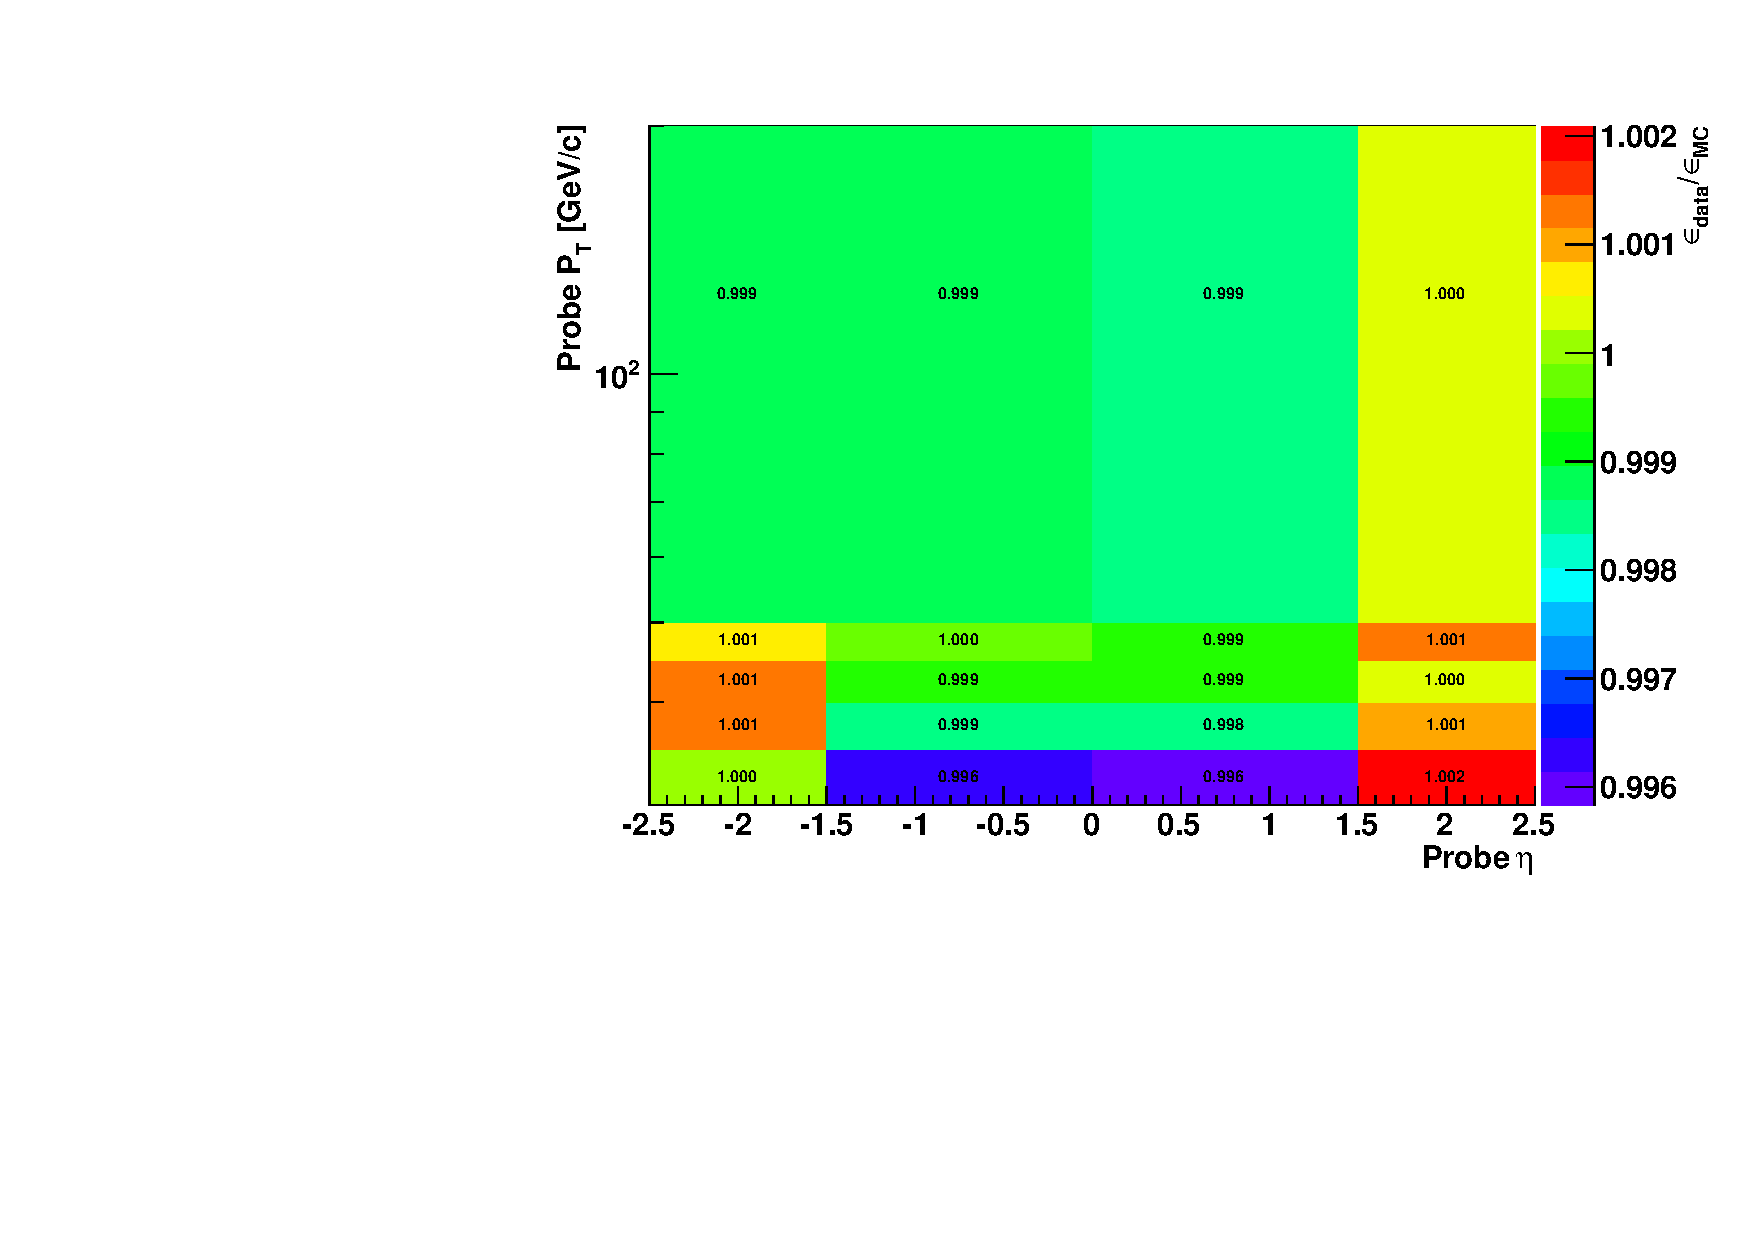
\includegraphics[width=0.32\textwidth]{figs/scaleFactor-Run2012ABC-SCToElectron.pdf}
  }
    \subfigure[]{
    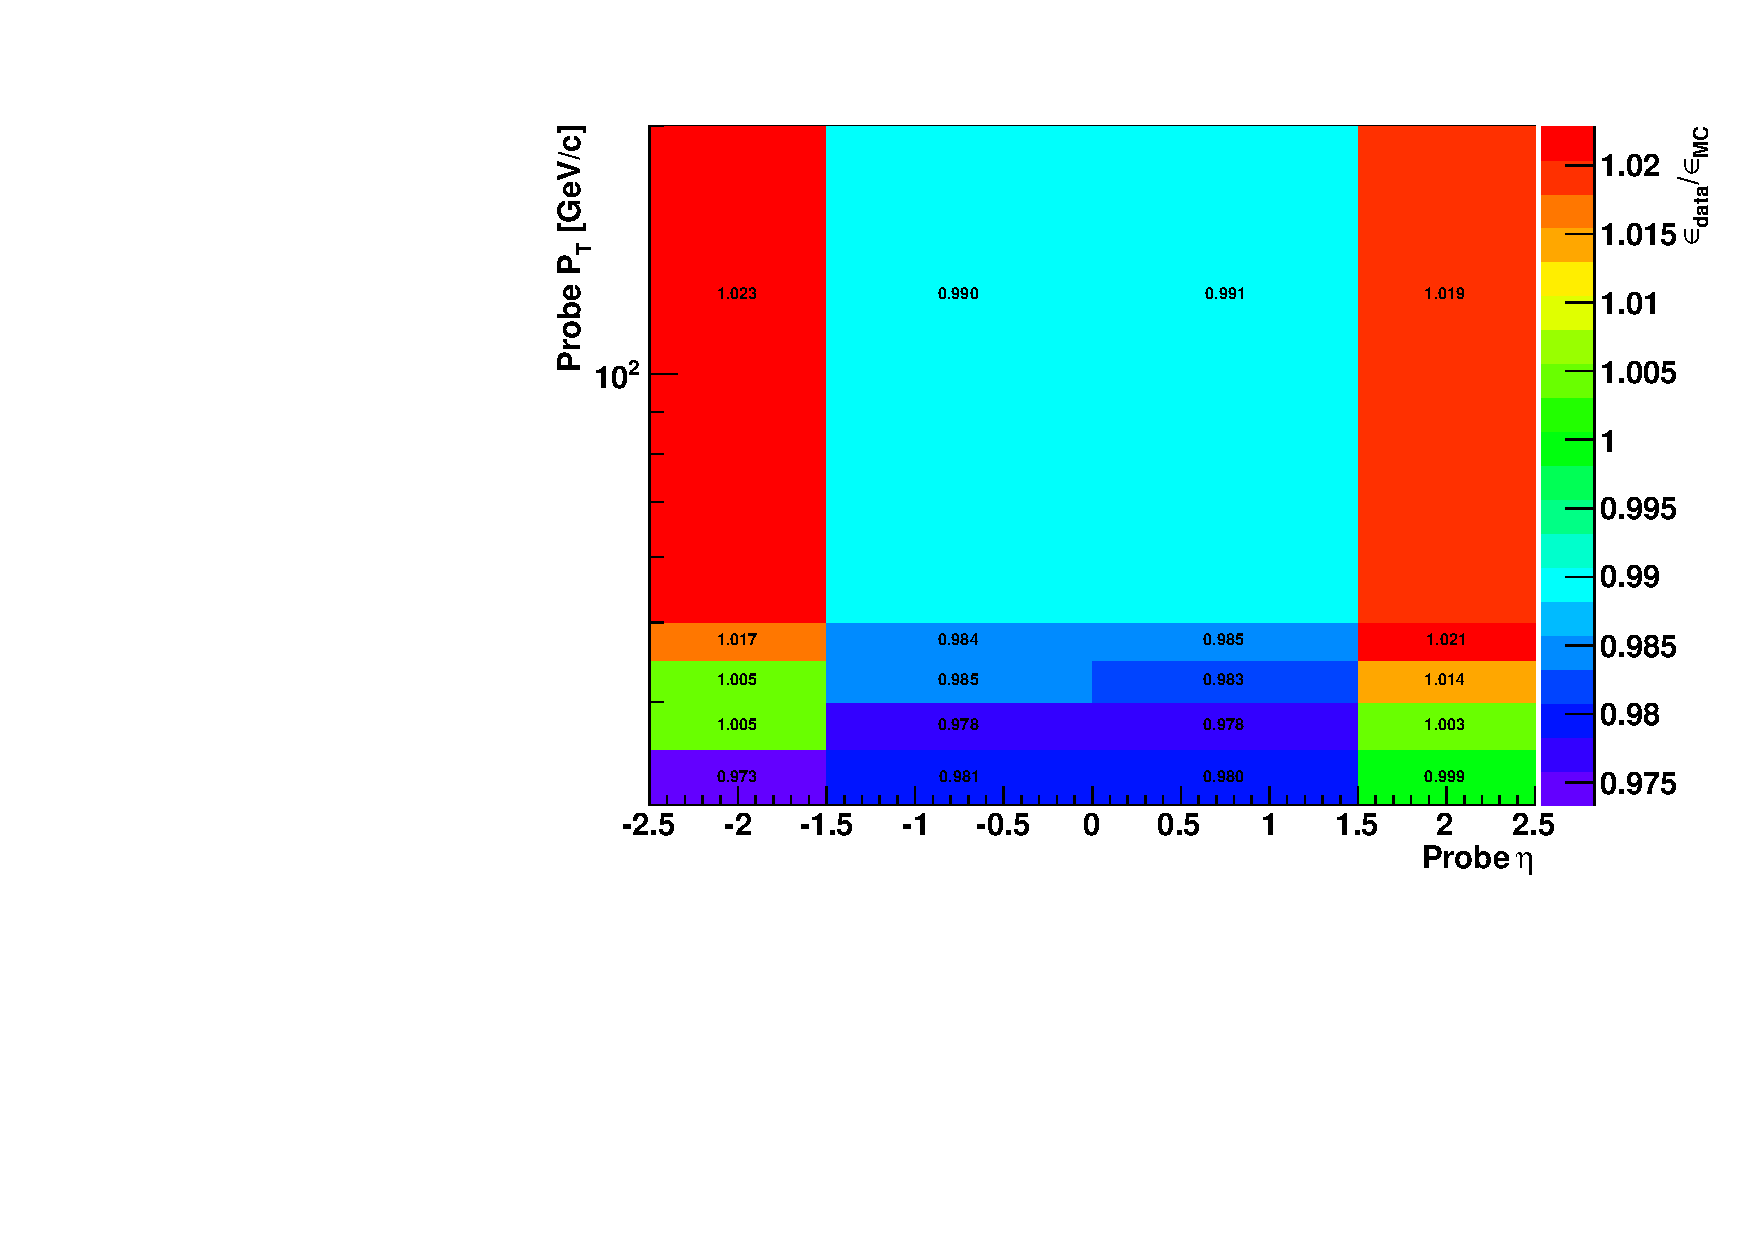
\includegraphics[width=0.32\textwidth]{figs/scaleFactor-Run2012ABC-GsfElectronToId.pdf}
  }
  \subfigure[]{
    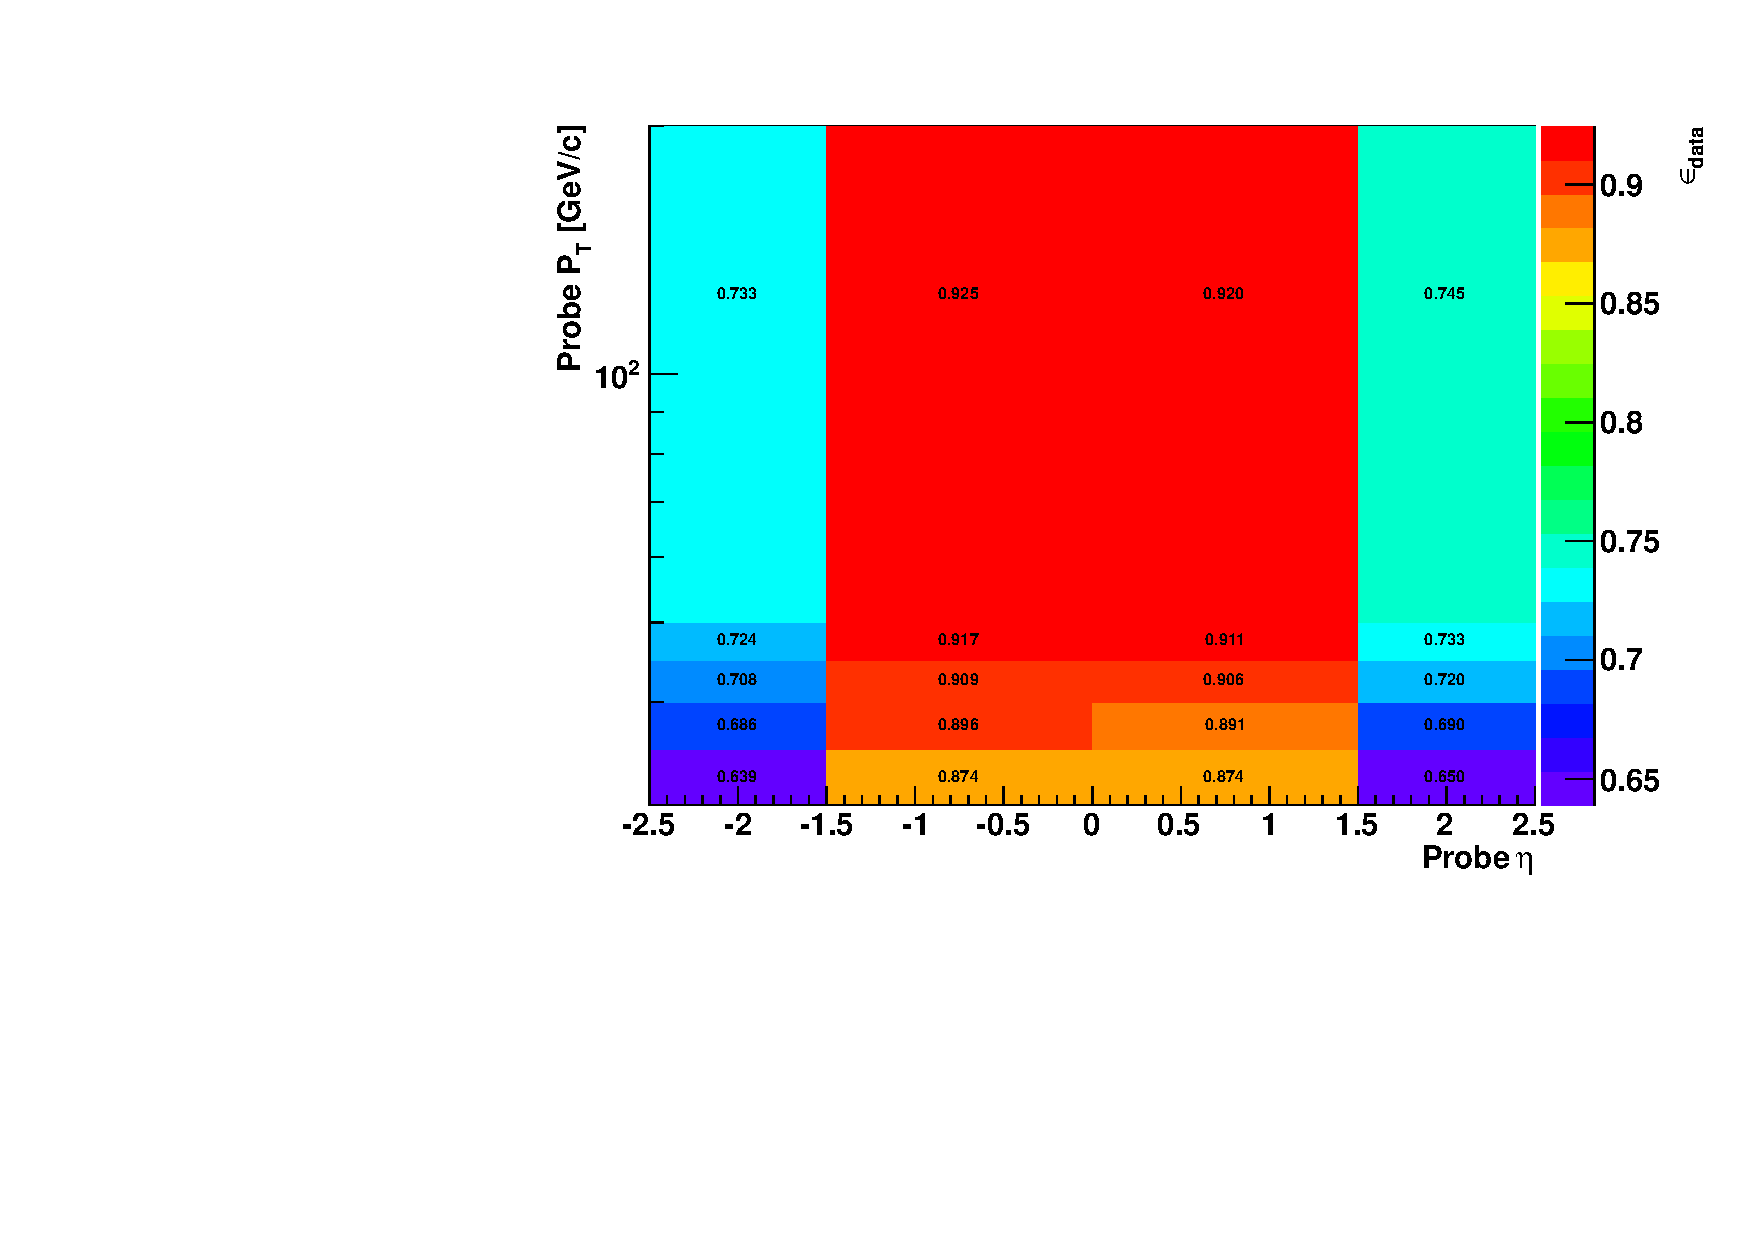
\includegraphics[width=0.32\textwidth]{figs/efficiency-Run2012ABC-WP80ToHLTEle.pdf}
  }
    \caption{Electron efficiency and data/MC scale factors for super-cluster to reconstructed electrons $\epsilon_{\textnormal{Reco}}$ (a),
    reconstructed to selected electrons $\epsilon_{\textnormal{Id}}$ (b) and selected to HLT electrons
      $\epsilon_{\textnormal{HLT}}$ (c).}
    \label{fig:eleEff}
  \end{center}
\end{figure}

\subsection{Muon efficiencies}\label{subsec:EffMu}

In the muon case, the reconstruction efficiency $\epsilon_{\textnormal{Reco}}$ describes the ability to reconstruct a Particle Flow muon starting with
a particle track and can be assumed to be one \cite{MUONPAS}. The identification efficiency $\epsilon_{\textnormal{Id}}$ gives an estimate for a
reconstructed muon to pass the offline selection criteria. It can be computed for both data and simulation and thus a scale factor being
the ratio of the two efficiencies is derived. \\
The trigger efficiency $\epsilon_{\textnormal{HLT}}$  is the fraction of selected muons fulfilling the HLT requirements and, since the HLT
requirement is dropped on the MC analysis, the efficiency computed on data is used directly to correct the MC event expectation.\\
The efficiency measurement is binned both in $\pt$ and $\eta$ of the probe muon covering the
relevant intervals (25, 30, 35, 40, 45, 50, 200)\GeVc in $\pt$ and (-2.1, -1.5, -1.0, -0.5, 0.0, 0.5, 1.0, 1.5, 2.1) in $\eta$. The resulting selection
and trigger efficiencies and scale factors are summarized in Table~\ref{tab:muonEff} and Figure~\ref{fig:muonEff}.

\begin{table}[htb]
\centering 
\scalebox{0.70}{
  \begin{tabular}{|c|c|c|c|c|c|}
  \hline
  $p_{\textnormal{T,min}}$ & $p_{\textnormal{T,max}}$ & $\eta_{\textnormal{min}}$ & $\eta_{\textnormal{max}}$ & $\epsilon_{\textnormal{ID,data}}$/$\epsilon_{\textnormal{ID,mc}}$ & $\epsilon_{\textnormal{HLT,data}}$ \\
  $[\GeVc]$         & $[\GeVc]$         &                     &                     &                             &                               \\
  \hline
  \hline
  25 & 30 & -2.1 & -1.5 & 0.992 $\pm$ 0.003 & 0.766 $\pm$ 0.003 \\
  25 & 30 & -1.5 & -1 & 0.987 $\pm$ 0.003 & 0.822 $\pm$ 0.003 \\
  25 & 30 & -1 & -0.5 & 0.990 $\pm$ 0.003 & 0.914 $\pm$ 0.002 \\
  25 & 30 & -0.5 & 0 & 0.984 $\pm$ 0.003 & 0.920 $\pm$ 0.002 \\
  25 & 30 & 0 & 0.5 & 0.985 $\pm$ 0.003 & 0.924 $\pm$ 0.002 \\
  25 & 30 & 0.5 & 1 & 0.992 $\pm$ 0.003 & 0.913 $\pm$ 0.002 \\
  25 & 30 & 1 & 1.5 & 0.991 $\pm$ 0.003 & 0.802 $\pm$ 0.003 \\
  25 & 30 & 1.5 & 2.1 & 0.995 $\pm$ 0.002 & 0.814 $\pm$ 0.003 \\
  30 & 35 & -2.1 & -1.5 & 0.991 $\pm$ 0.002 & 0.785 $\pm$ 0.002 \\
  30 & 35 & -1.5 & -1 & 0.988 $\pm$ 0.002 & 0.829 $\pm$ 0.002 \\
  30 & 35 & -1 & -0.5 & 0.988 $\pm$ 0.002 & 0.921 $\pm$ 0.002 \\
  30 & 35 & -0.5 & 0 & 0.984 $\pm$ 0.002 & 0.930 $\pm$ 0.001 \\
  30 & 35 & 0 & 0.5 & 0.985 $\pm$ 0.002 & 0.935 $\pm$ 0.001 \\
  30 & 35 & 0.5 & 1 & 0.990 $\pm$ 0.002 & 0.922 $\pm$ 0.002 \\
  30 & 35 & 1 & 1.5 & 0.987 $\pm$ 0.002 & 0.807 $\pm$ 0.002 \\
  30 & 35 & 1.5 & 2.1 & 0.995 $\pm$ 0.002 & 0.833 $\pm$ 0.002 \\
  35 & 40 & -2.1 & -1.5 & 0.992 $\pm$ 0.002 & 0.793 $\pm$ 0.002 \\
  35 & 40 & -1.5 & -1 & 0.987 $\pm$ 0.002 & 0.832 $\pm$ 0.002 \\
  35 & 40 & -1 & -0.5 & 0.991 $\pm$ 0.002 & 0.926 $\pm$ 0.001 \\
  35 & 40 & -0.5 & 0 & 0.986 $\pm$ 0.002 & 0.935 $\pm$ 0.001 \\
  35 & 40 & 0 & 0.5 & 0.986 $\pm$ 0.002 & 0.940 $\pm$ 0.001 \\
  35 & 40 & 0.5 & 1 & 0.991 $\pm$ 0.002 & 0.925 $\pm$ 0.001 \\
  35 & 40 & 1 & 1.5 & 0.989 $\pm$ 0.002 & 0.812 $\pm$ 0.002 \\
  35 & 40 & 1.5 & 2.1 & 0.994 $\pm$ 0.002 & 0.837 $\pm$ 0.002 \\
  40 & 45 & -2.1 & -1.5 & 0.994 $\pm$ 0.002 & 0.800 $\pm$ 0.002 \\
  40 & 45 & -1.5 & -1 & 0.987 $\pm$ 0.001 & 0.837 $\pm$ 0.002 \\
  40 & 45 & -1 & -0.5 & 0.992 $\pm$ 0.001 & 0.927 $\pm$ 0.001 \\
  40 & 45 & -0.5 & 0 & 0.986 $\pm$ 0.001 & 0.940 $\pm$ 0.001 \\
  40 & 45 & 0 & 0.5 & 0.987 $\pm$ 0.001 & 0.944 $\pm$ 0.001 \\
  40 & 45 & 0.5 & 1 & 0.991 $\pm$ 0.001 & 0.928 $\pm$ 0.001 \\
  40 & 45 & 1 & 1.5 & 0.991 $\pm$ 0.001 & 0.817 $\pm$ 0.002 \\
  40 & 45 & 1.5 & 2.1 & 0.996 $\pm$ 0.001 & 0.844 $\pm$ 0.002 \\
  45 & 50 & -2.1 & -1.5 & 0.993 $\pm$ 0.002 & 0.807 $\pm$ 0.002 \\
  45 & 50 & -1.5 & -1 & 0.987 $\pm$ 0.002 & 0.840 $\pm$ 0.002 \\
  45 & 50 & -1 & -0.5 & 0.990 $\pm$ 0.001 & 0.931 $\pm$ 0.001 \\
  45 & 50 & -0.5 & 0 & 0.988 $\pm$ 0.002 & 0.941 $\pm$ 0.001 \\
  45 & 50 & 0 & 0.5 & 0.987 $\pm$ 0.002 & 0.947 $\pm$ 0.001 \\
  45 & 50 & 0.5 & 1 & 0.992 $\pm$ 0.001 & 0.930 $\pm$ 0.001 \\
  45 & 50 & 1 & 1.5 & 0.991 $\pm$ 0.002 & 0.821 $\pm$ 0.002 \\
  45 & 50 & 1.5 & 2.1 & 0.995 $\pm$ 0.002 & 0.851 $\pm$ 0.002 \\
  50 & 200 & -2.1 & -1.5 & 0.991 $\pm$ 0.002 & 0.809 $\pm$ 0.002 \\
  50 & 200 & -1.5 & -1 & 0.987 $\pm$ 0.002 & 0.842 $\pm$ 0.002 \\
  50 & 200 & -1 & -0.5 & 0.992 $\pm$ 0.002 & 0.931 $\pm$ 0.001 \\
  50 & 200 & -0.5 & 0 & 0.987 $\pm$ 0.002 & 0.944 $\pm$ 0.001 \\
  50 & 200 & 0 & 0.5 & 0.989 $\pm$ 0.002 & 0.946 $\pm$ 0.001 \\
  50 & 200 & 0.5 & 1 & 0.992 $\pm$ 0.002 & 0.932 $\pm$ 0.001 \\
  50 & 200 & 1 & 1.5 & 0.993 $\pm$ 0.002 & 0.824 $\pm$ 0.002 \\
  50 & 200 & 1.5 & 2.1 & 0.996 $\pm$ 0.002 & 0.854 $\pm$ 0.002 \\
  \hline
  \end{tabular}}
\caption{Muon selection scale factors and HLT efficiencies. The errors are statistical only.} 
\label{tab:muonEff} 
\end{table}

\begin{figure}[t]
  \begin{center}
    \subfigure[]{
    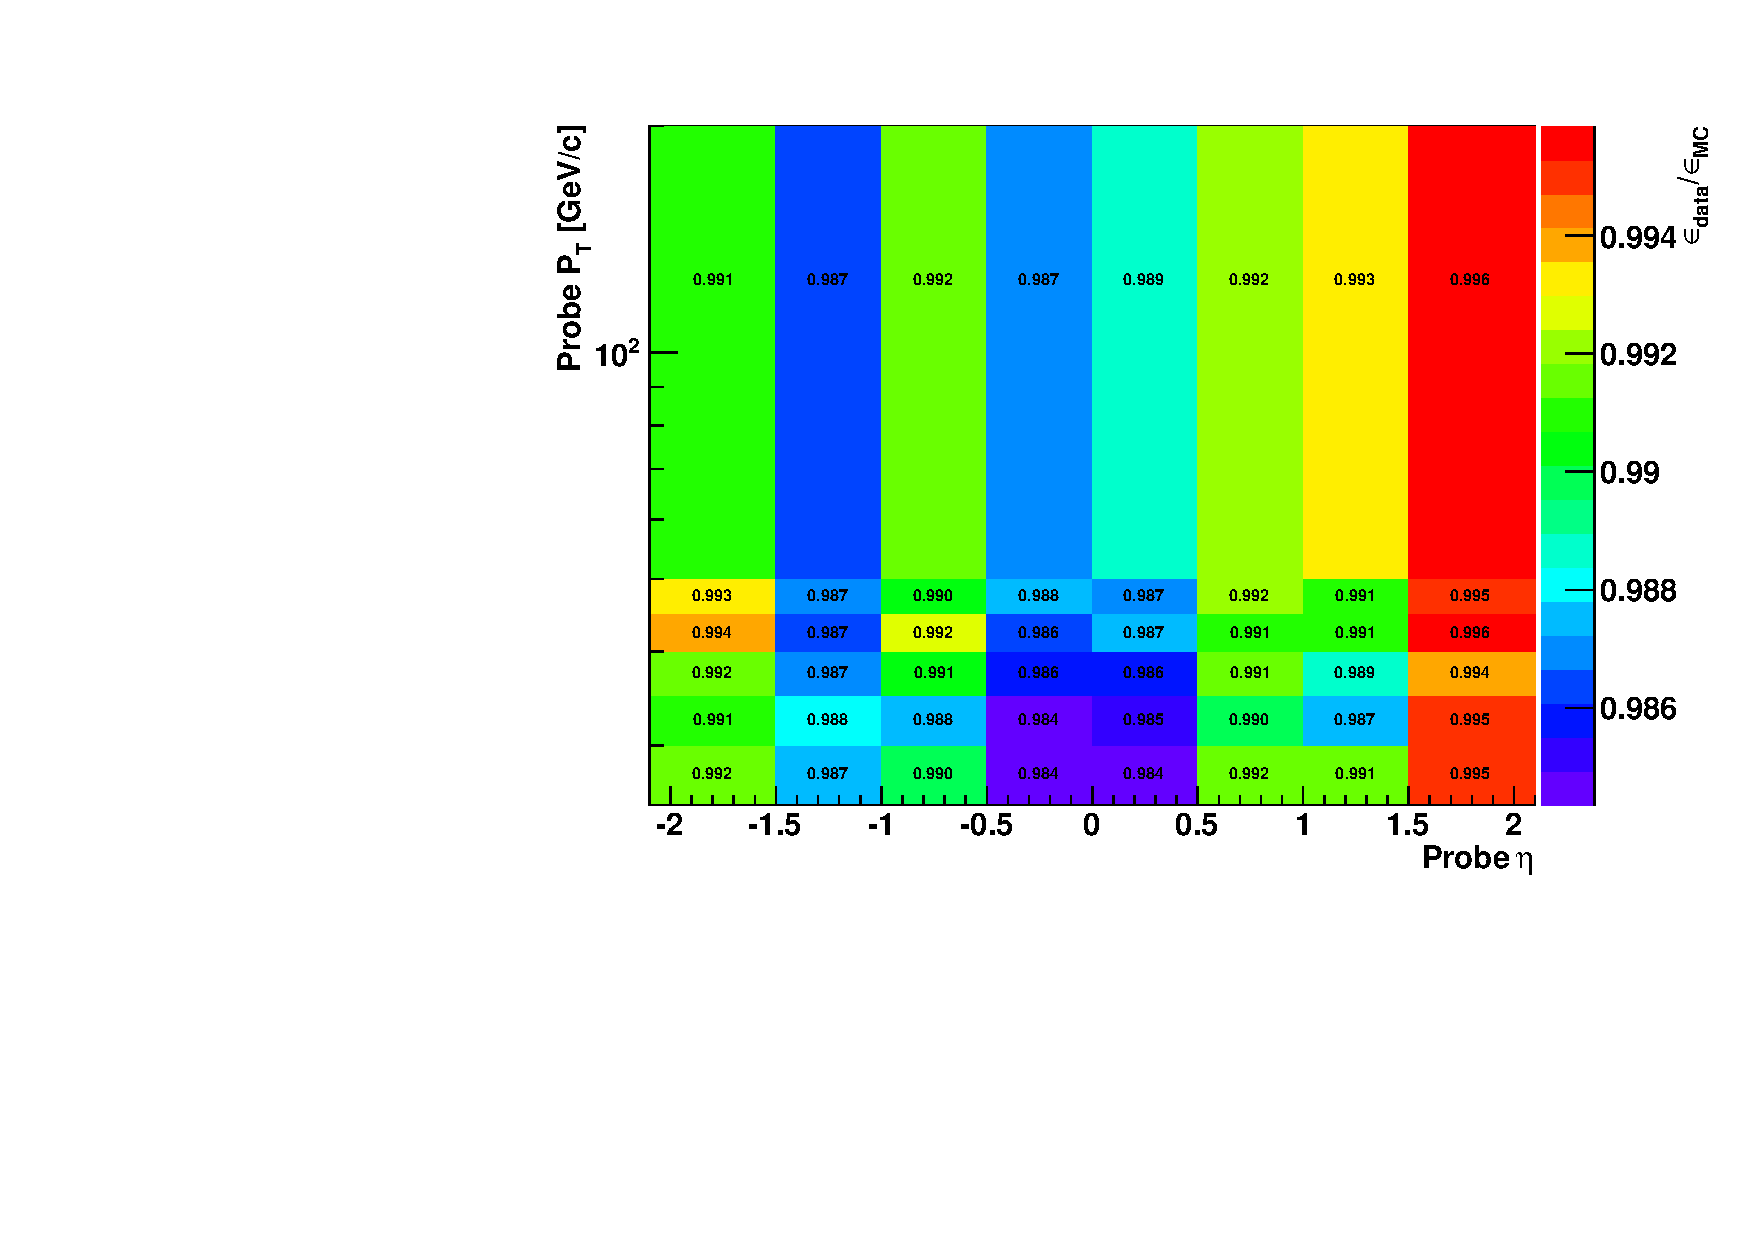
\includegraphics[width=0.47\textwidth]{figs/scaleFactor-Run2012ABC-RecoToIso.pdf}
  }
  \subfigure[]{
    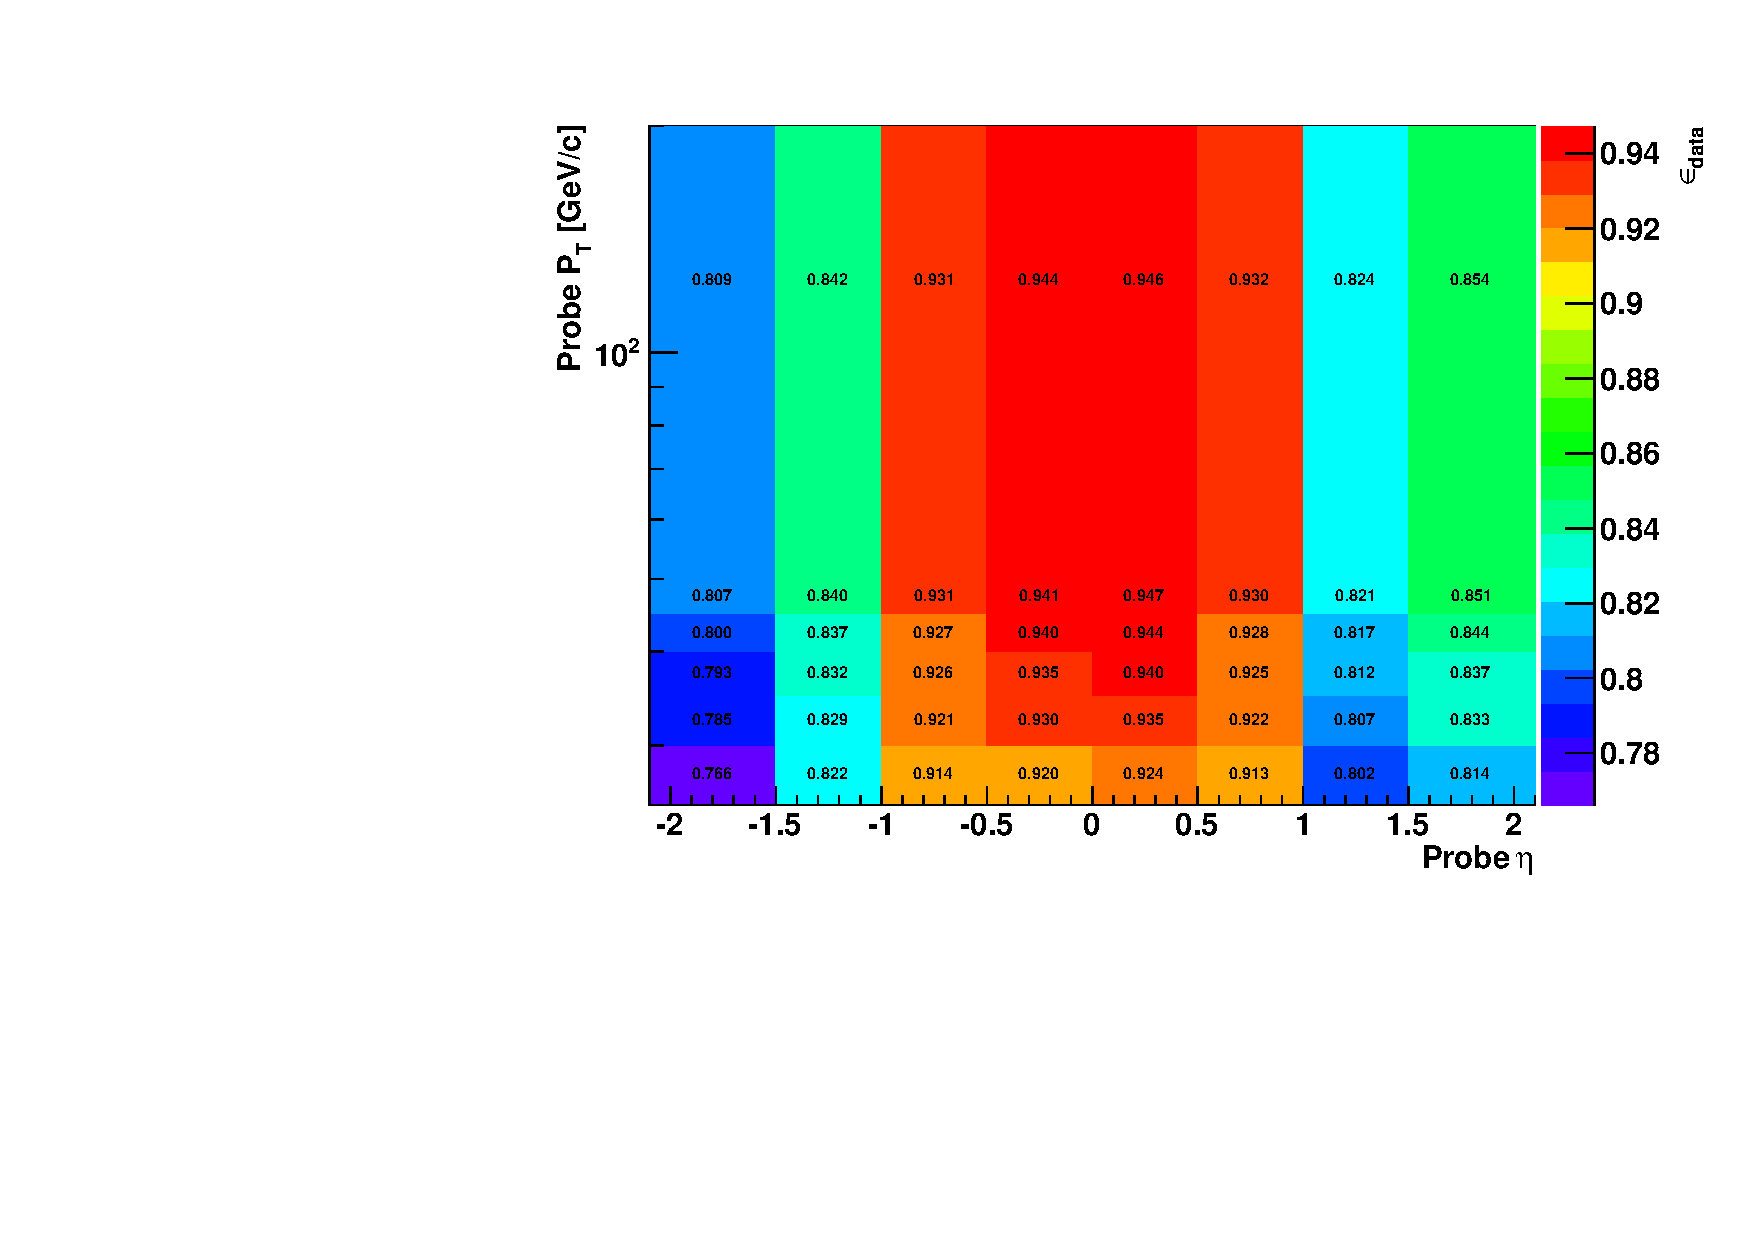
\includegraphics[width=0.47\textwidth]{figs/efficiency-Run2012ABC-IsoToIsoMuHLT.pdf}
  }
    \caption{Muon scale factors for reconstructed to selected muons $\epsilon_{\textnormal{ID,data}}$/$\epsilon_{\textnormal{ID,mc}}$ (a) and 
    efficiency for selected to HLT muons $\epsilon_{\textnormal{HLT,data}}$ (b).}
    \label{fig:muonEff}
  \end{center}
\end{figure}

%%%%%%%%%%%%%%%%%%%%%%%%%%%%%%%%%%%%%%%%%%%%%%%%%%%%%%%%%%%%%%%%%%%%
%%%%%%%%%%%%%%%%%%%%%%%%%%%%%%%%%%%%%%%%%%%%%%%%%%%%%%%%%%%%%%%%%%%%
\section{Effect of pileup}
\label{sec:pileup}
The presence of additional interactions, known as Pile-up (PU), is expected to affect
this analysis in the following ways:
%%%%%
\begin{itemize}
\item additional energy deposits from PU will be added to the jets from the main 
interaction
\item additional low $p_{T}$ jets composed of PU energy will be
added to the event
\item tracks and calorimetric towers from PU energy deposits will be
added to the isolation energy sum of the lepton, thus making isolation 
cuts less efficient.
\end{itemize}
%%%%%
Particle flow (PF) algorithms can be used to decrease the effects of pileup. 
Charged PF particles with tracks pointing to non-primary 
vertices are removed from the list of particles used to reconstruct jets. 
Neutral particles do not leave tracks, and therefore cannot be associated with
a vertex and removed. 

\par
Various techniques have been developed and centrally validated in CMS to 
alleviate the degradation in object reconstruction due to PU effects.
The present analysis makes full use of these improvements. 
The so-called Fastjet and L1-offset corrections remove the additional 
energy released in the event from PU interactions.
The charged particles coming from PU are removed prior to 
jet clustering by requiring that all the tracks come from the primary vertex. 
Similarly, for leptons we subtract from the isolation 
energy sum the pileup contribution from charged particles.
As a result of these corrections, 
the effect of pile-up reweighing in the analysis should be small.
The Summer12 Monte Carlo samples have been corrected, with a reweighing factor obtained from the comparison of 
the number of vertices in data and in Monte Carlo. 
%The good agreement of primary vertex distribution between data and MC after PU re-weighting is shown in Fig.~\ref{fig:pu_MCcomp}.
%The effect of PU on the $m_{jj}$ shape from the W+jets Monte Carlo is 
%shown in section~10 of CMS AN-2011/266 as well as in Fig.~\ref{fig:pu_MCcomp} for 8~TeV, in which the dijet mass distribution 
%is shown before and after the PU correction. 
%We conclude from the plot that the effect of pileup is statistically insignificant.

%%%%%%%
\begin{figure}[h!] {\centering
\unitlength=0.33\linewidth
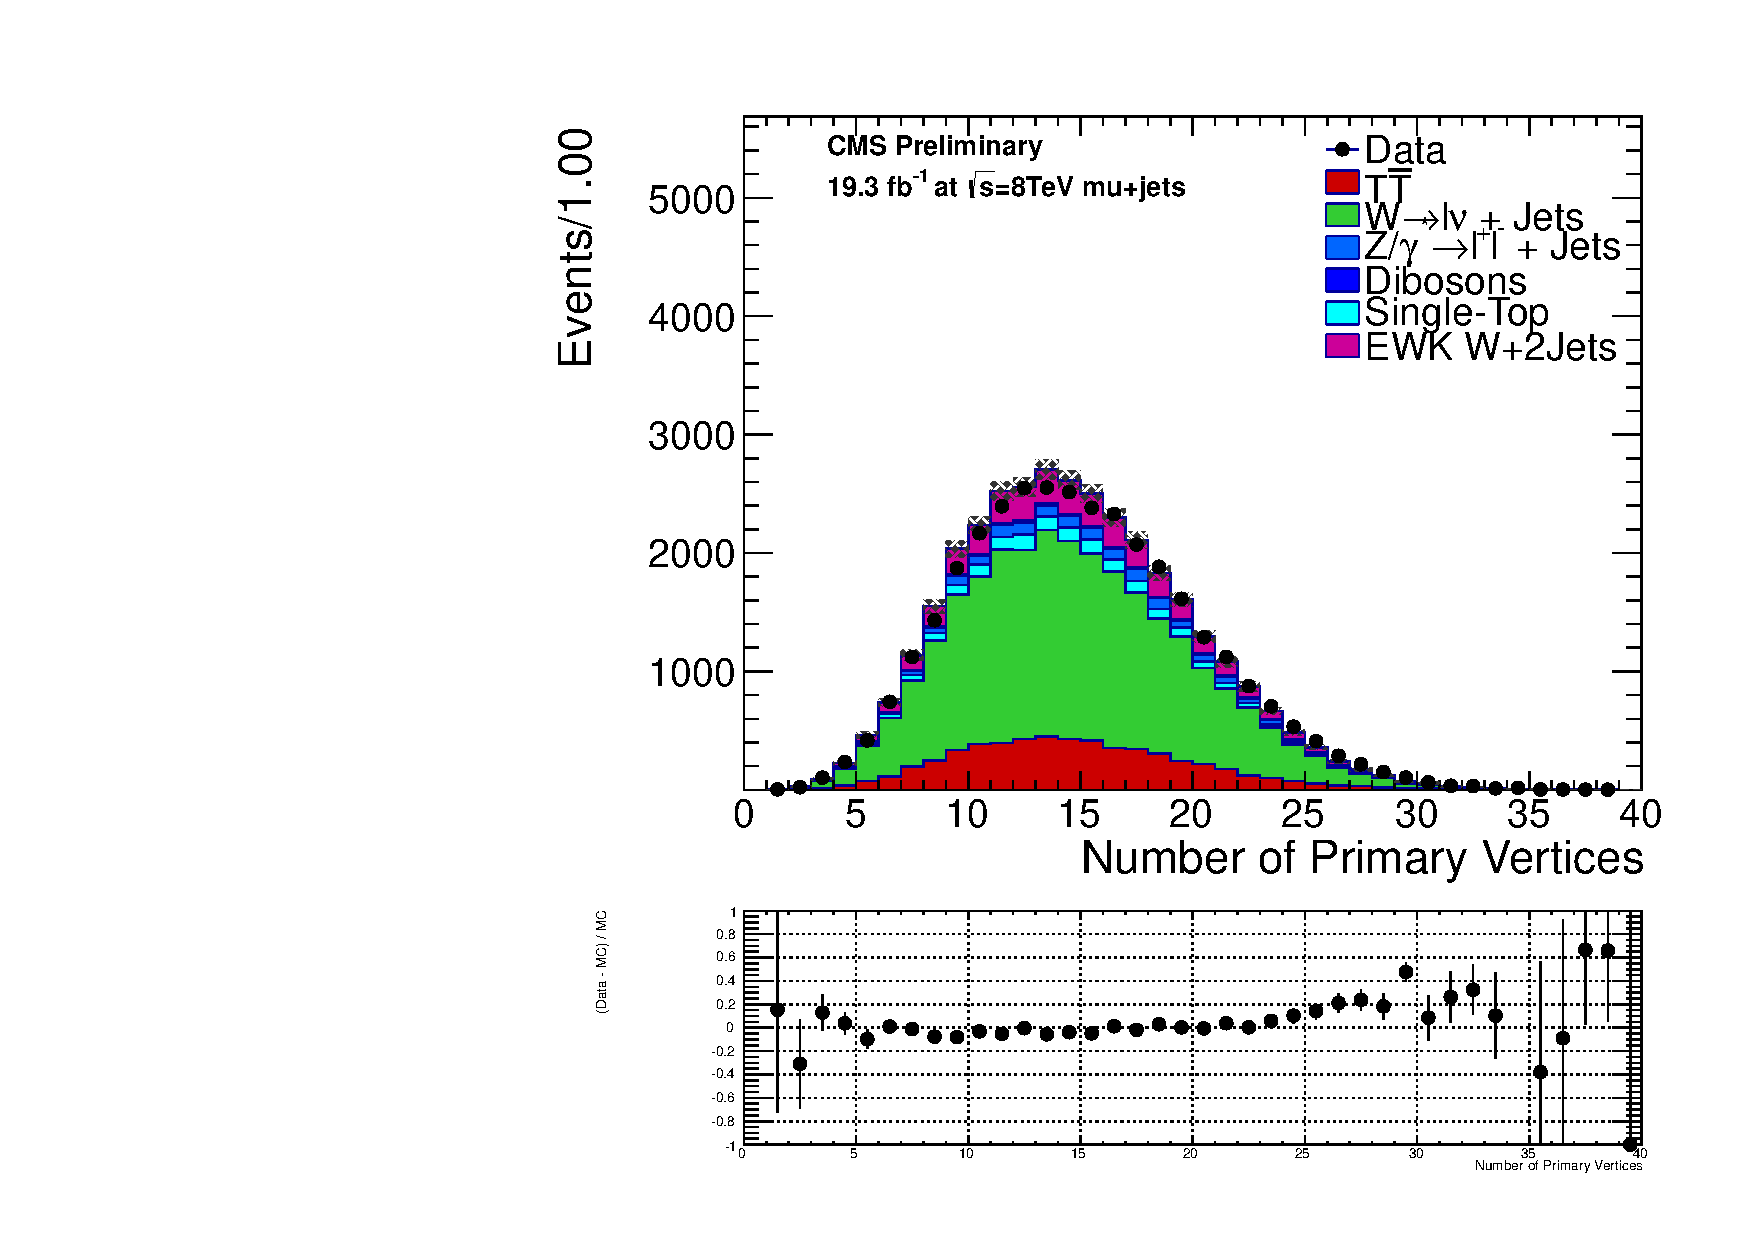
\includegraphics[width=0.48\textwidth]{figs/n-1_plots_mu/mu_event_nPV_mjj_600_tagjet1_60_tagjet2_50_Zeppenfield_1point2_EWKW2jets.pdf}
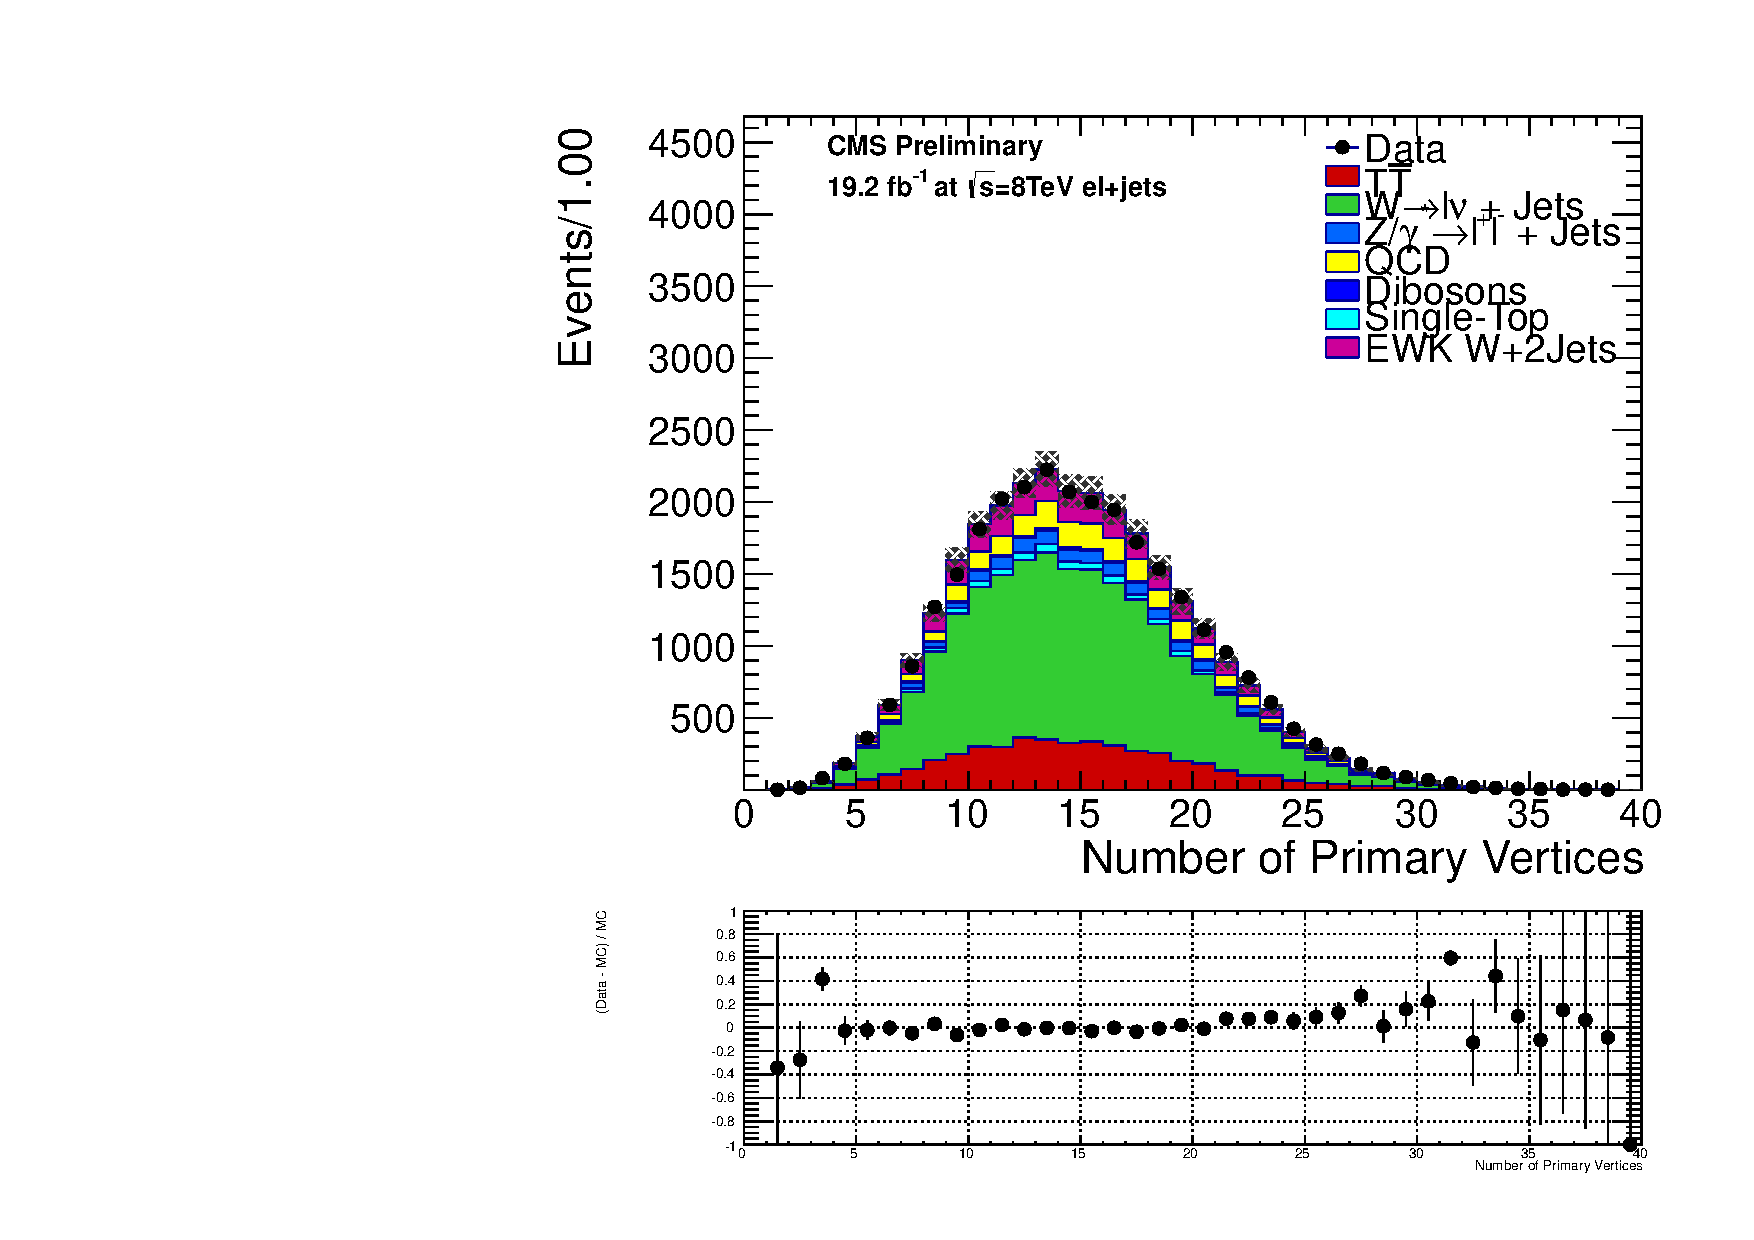
\includegraphics[width=0.48\textwidth]{figs/n-1_plots_el/el_event_nPV_mjj_600_tagjet1_60_tagjet2_50_Zeppenfield_1point2_met_30_WmT_30_EWKW2jets.pdf}
\caption{Primary vertex distribution after PU re-weighting: muons (left) and electrons (right).
%PU re-weighting according to the number of primary vertices in the event. 
%After correcting for the different area of both distributions.
%The ratio of the two distributions is consistent with unity.
} 
\label{fig:pu_MCcomp}}
\end{figure}
%%%%%%%
The good agreement of primary vertex distribution between data and MC after PU re-weighting is shown in Fig.~\ref{fig:pu_MCcomp}. Specifically, the leading jet $p_{T}$, the second leading jet $p_{T}$ and tagjet pair invariant mass $m_{jj}$ comparisons are shown in Figs.~\ref{fig:pu_mjjLow}-\ref{fig:pu_jet2ldHigh} for low (NPV$<12$) and high (NPV$>12$) PU scenarios are shown. Reasonable agreement is found in these two PU cases (within statistics).
%%%%%%%%%%%%%%%%%%%%%%%%%%%%
%%%%%%%
\begin{figure}[h!t]
  {\centering
    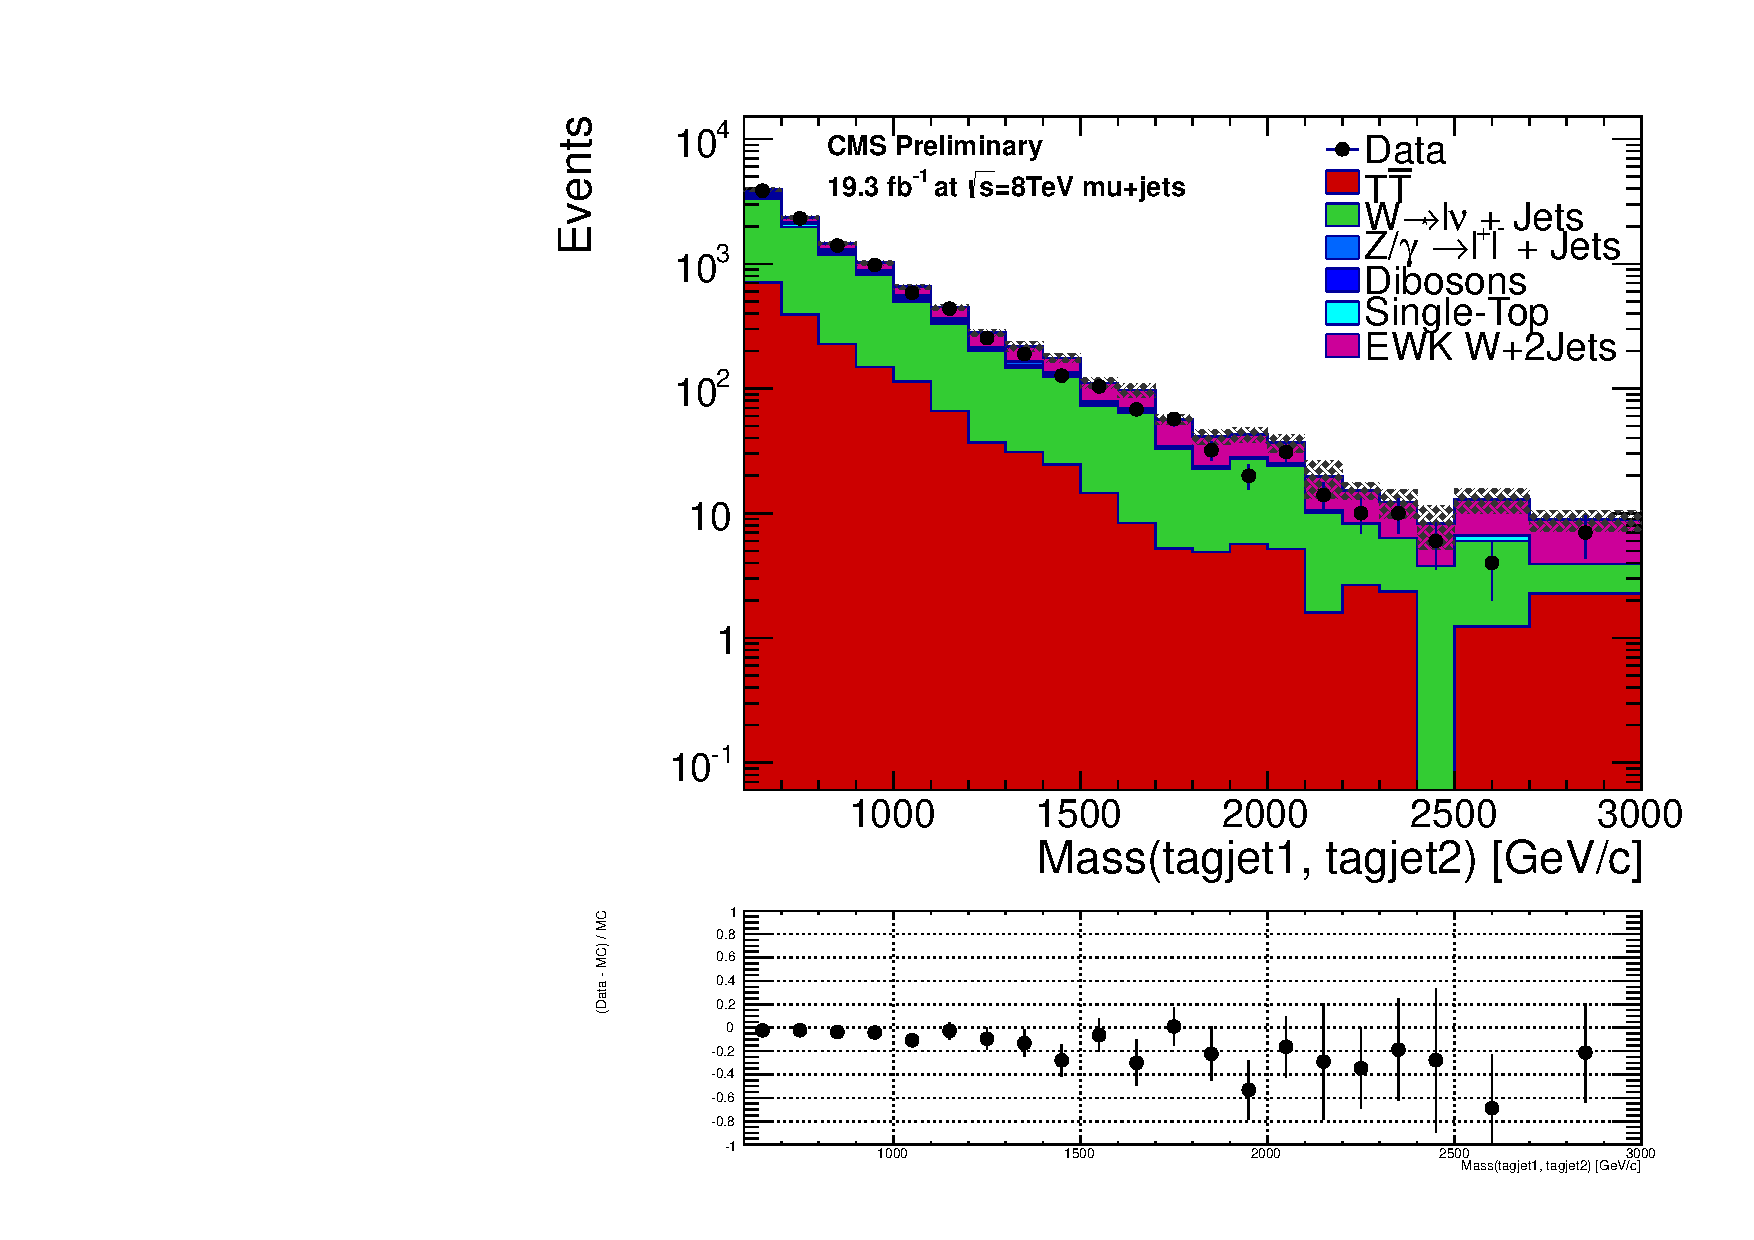
\includegraphics[width=0.49\textwidth]{figs/puchecks/mu_EWK_W_2jets_tagjet_mass_mjj_600_tagjet1_60_tagjet2_50_Zeppenfield_1point2_nPV_12_logy_rebin_EWKW2jets.pdf}
    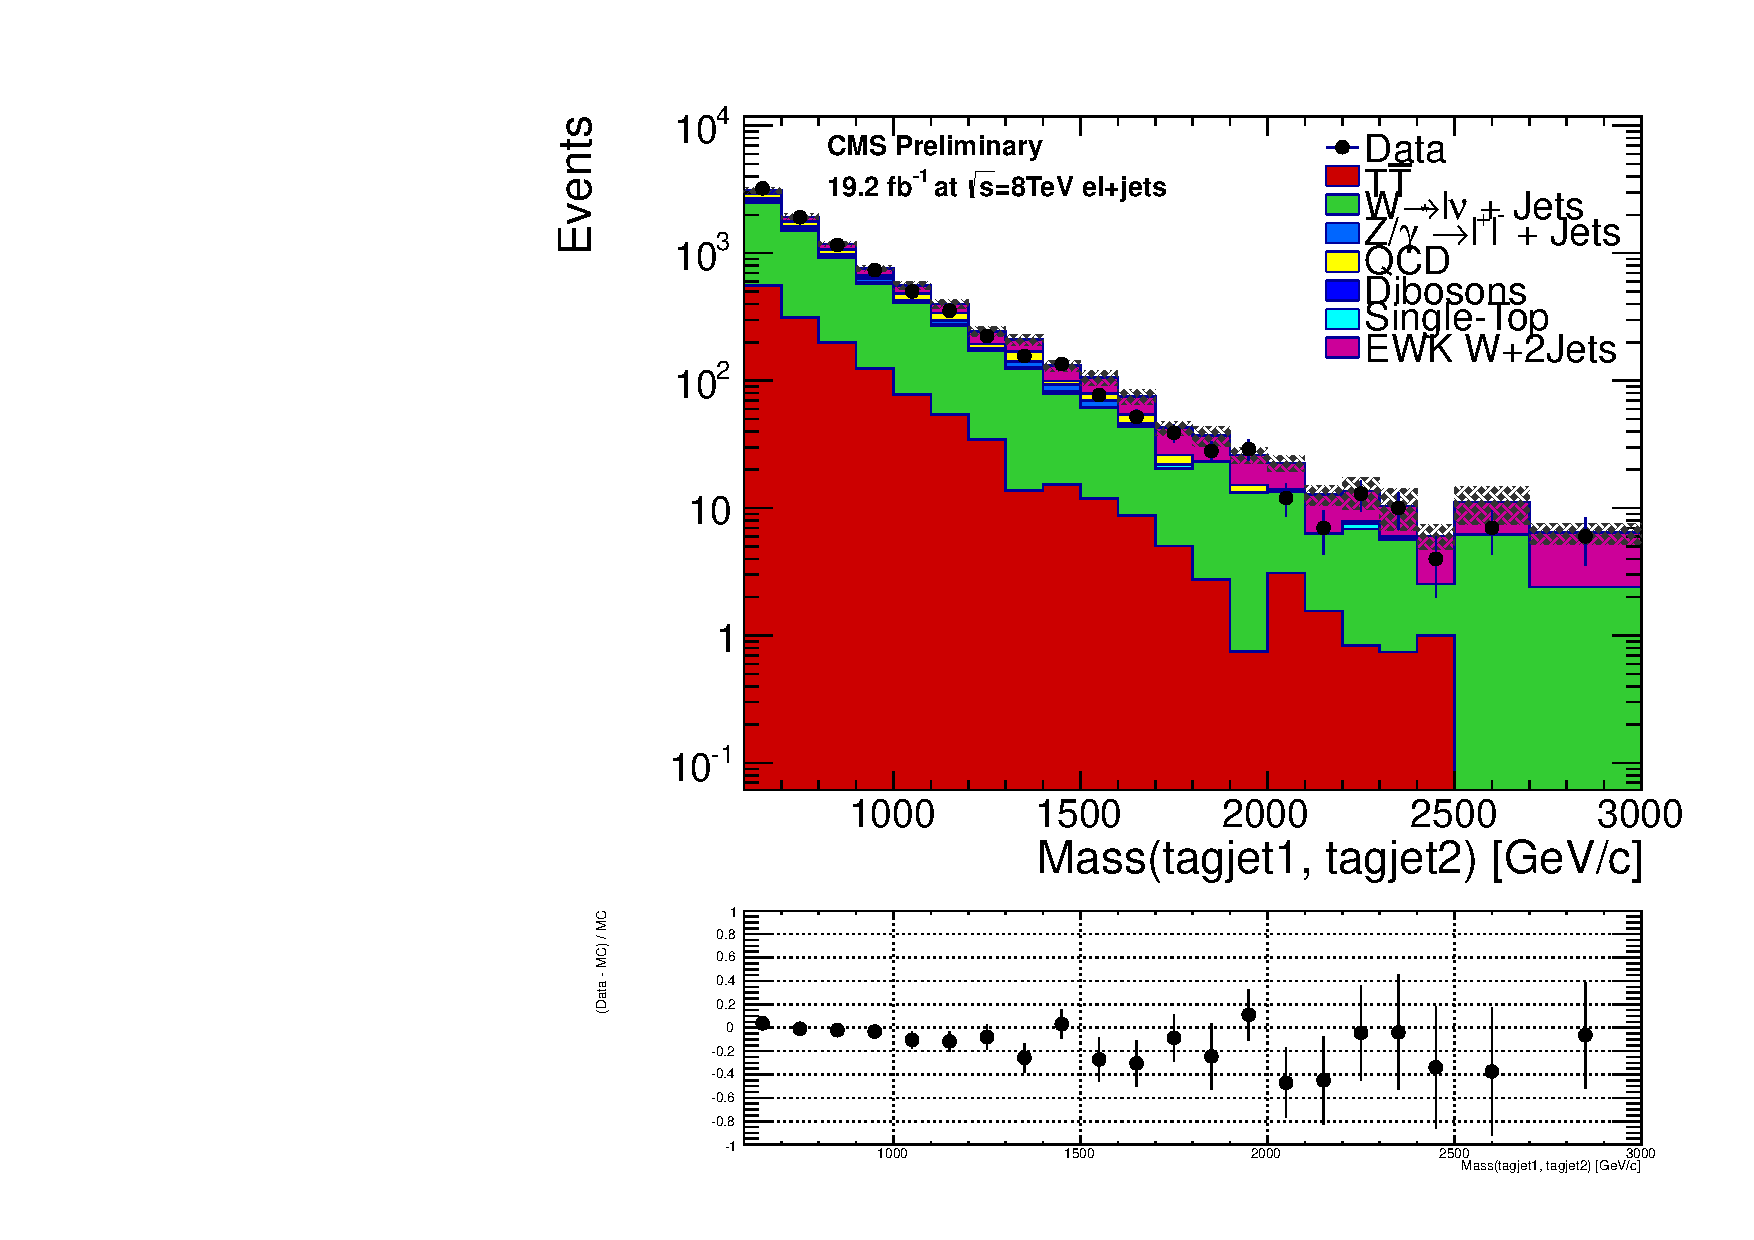
\includegraphics[width=0.49\textwidth]{figs/puchecks/el_EWK_W_2jets_tagjet_mass_mjj_600_tagjet1_60_tagjet2_50_Zeppenfield_1point2_nPV_12_met_30_WmT_30_logy_rebin_EWKW2jets.pdf}
    \caption{Comparison of the distributions from data and MC of the
    tagjet pair invariant mass for muons (left) and electrons (right)
    in Low (NPV$<12$) PileUp dijet events.}
\label{fig:pu_mjjLow}}
\end{figure}
%%%%%%%
%%%%%%%
\begin{figure}[h!t]
  {\centering
    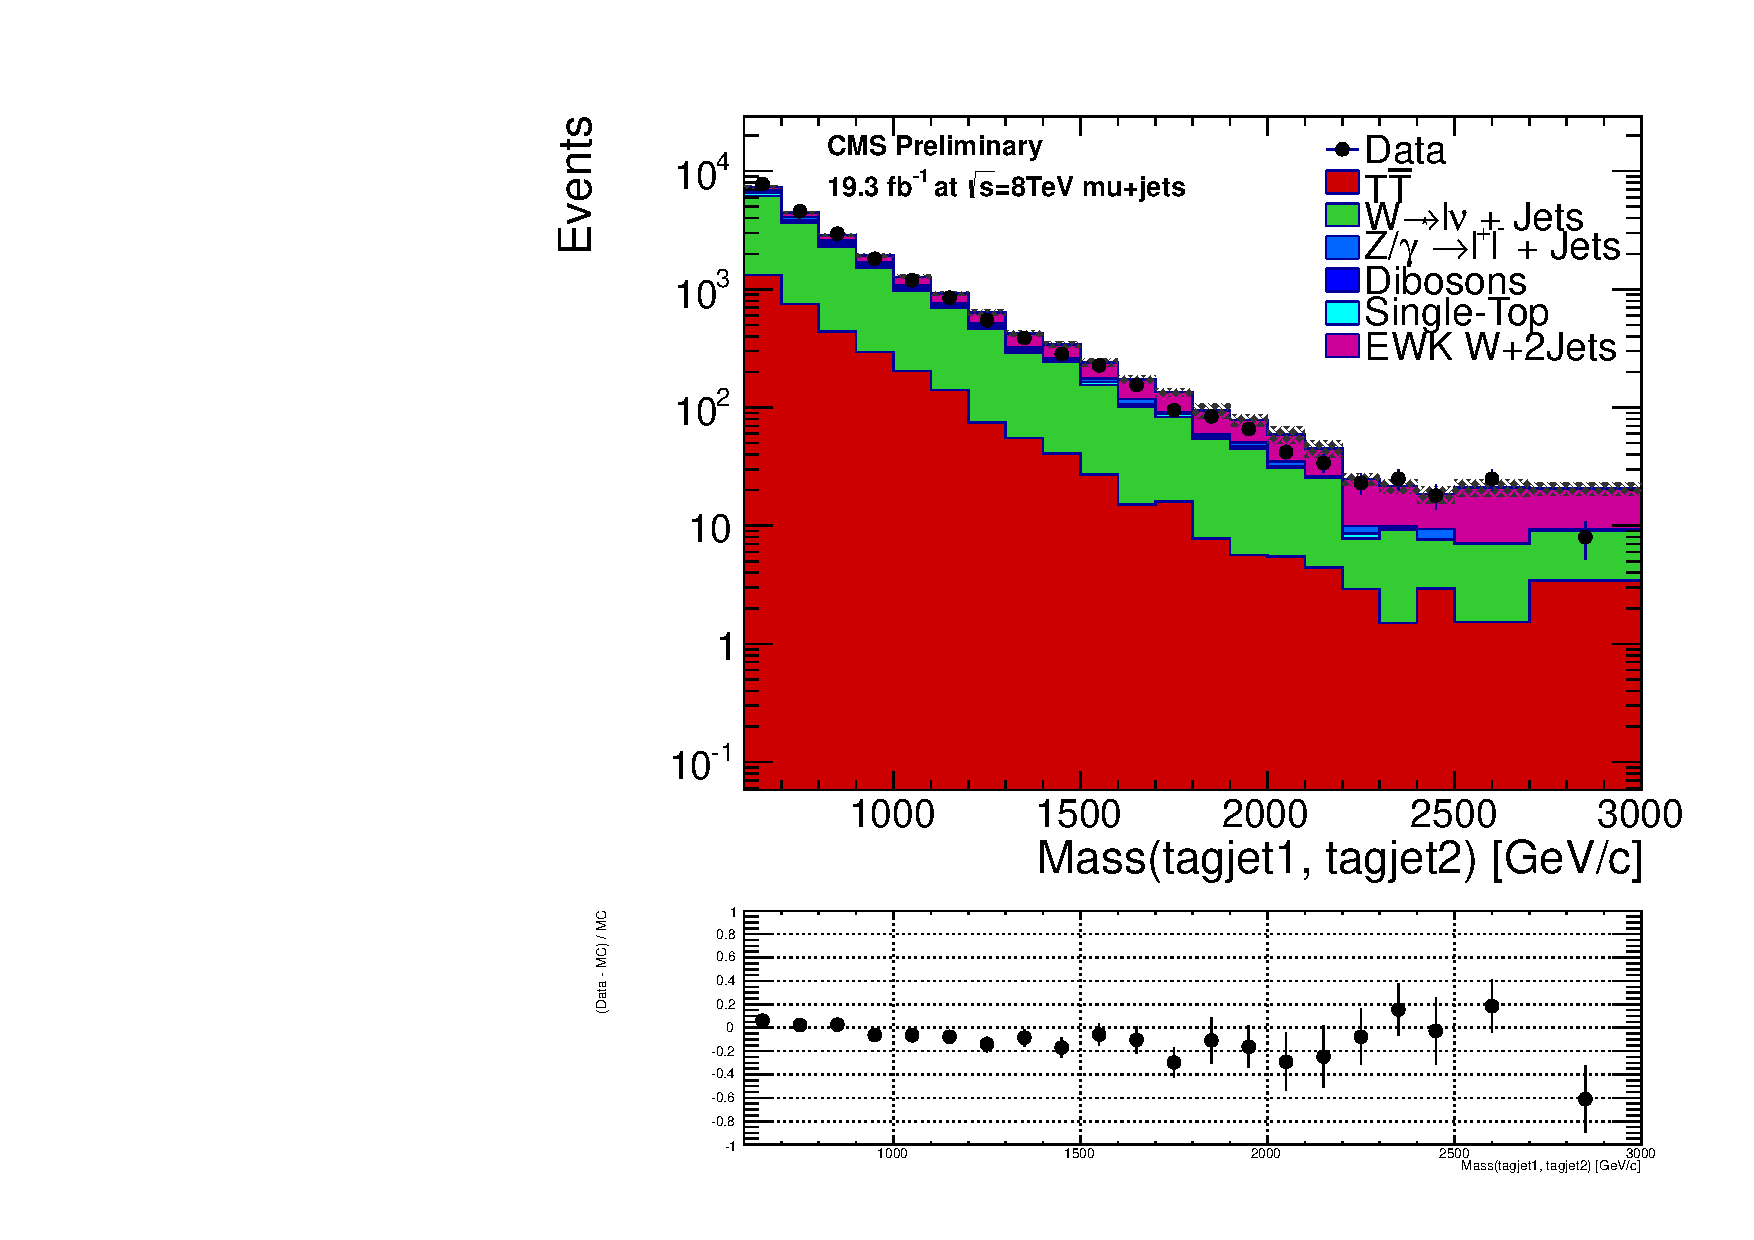
\includegraphics[width=0.49\textwidth]{figs/puchecks/mu_EWK_W_2jets_tagjet_mass_mjj_600_tagjet1_60_tagjet2_50_Zeppenfield_1point2_nPV_large_12_logy_rebin_EWKW2jets.pdf}
    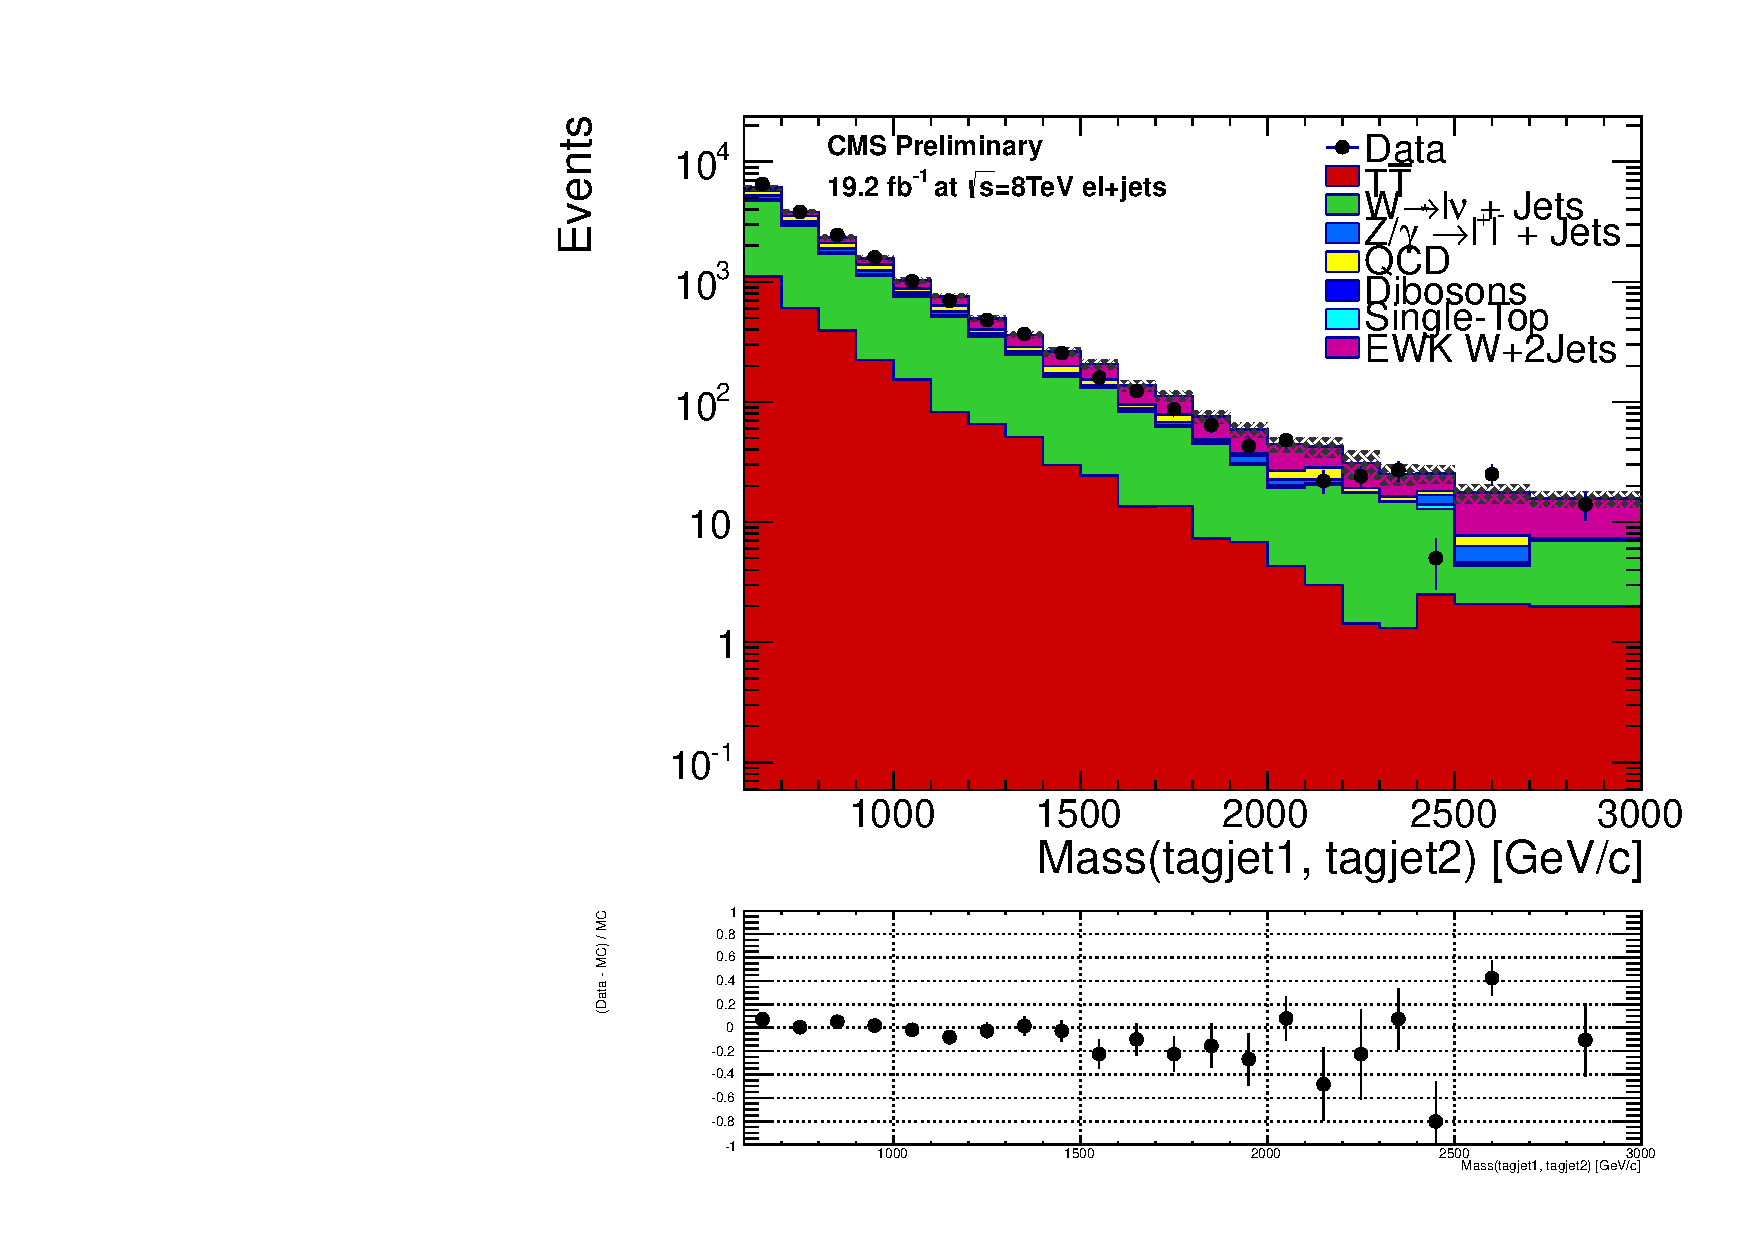
\includegraphics[width=0.49\textwidth]{figs/puchecks/el_EWK_W_2jets_tagjet_mass_mjj_600_tagjet1_60_tagjet2_50_Zeppenfield_1point2_nPV_large_12_met_30_WmT_30_logy_rebin_EWKW2jets.pdf}
    \caption{Comparison of the distributions from data and MC of the
    tagjet pair invariant mass for muons (left) and electrons (right)
    in High (NPV$>12$) PileUp events.}
\label{fig:pu_mjjHigh}}
\end{figure}
%%%%%%%
%%%%%%% jetld
\begin{figure}[h!t]
  {\centering
    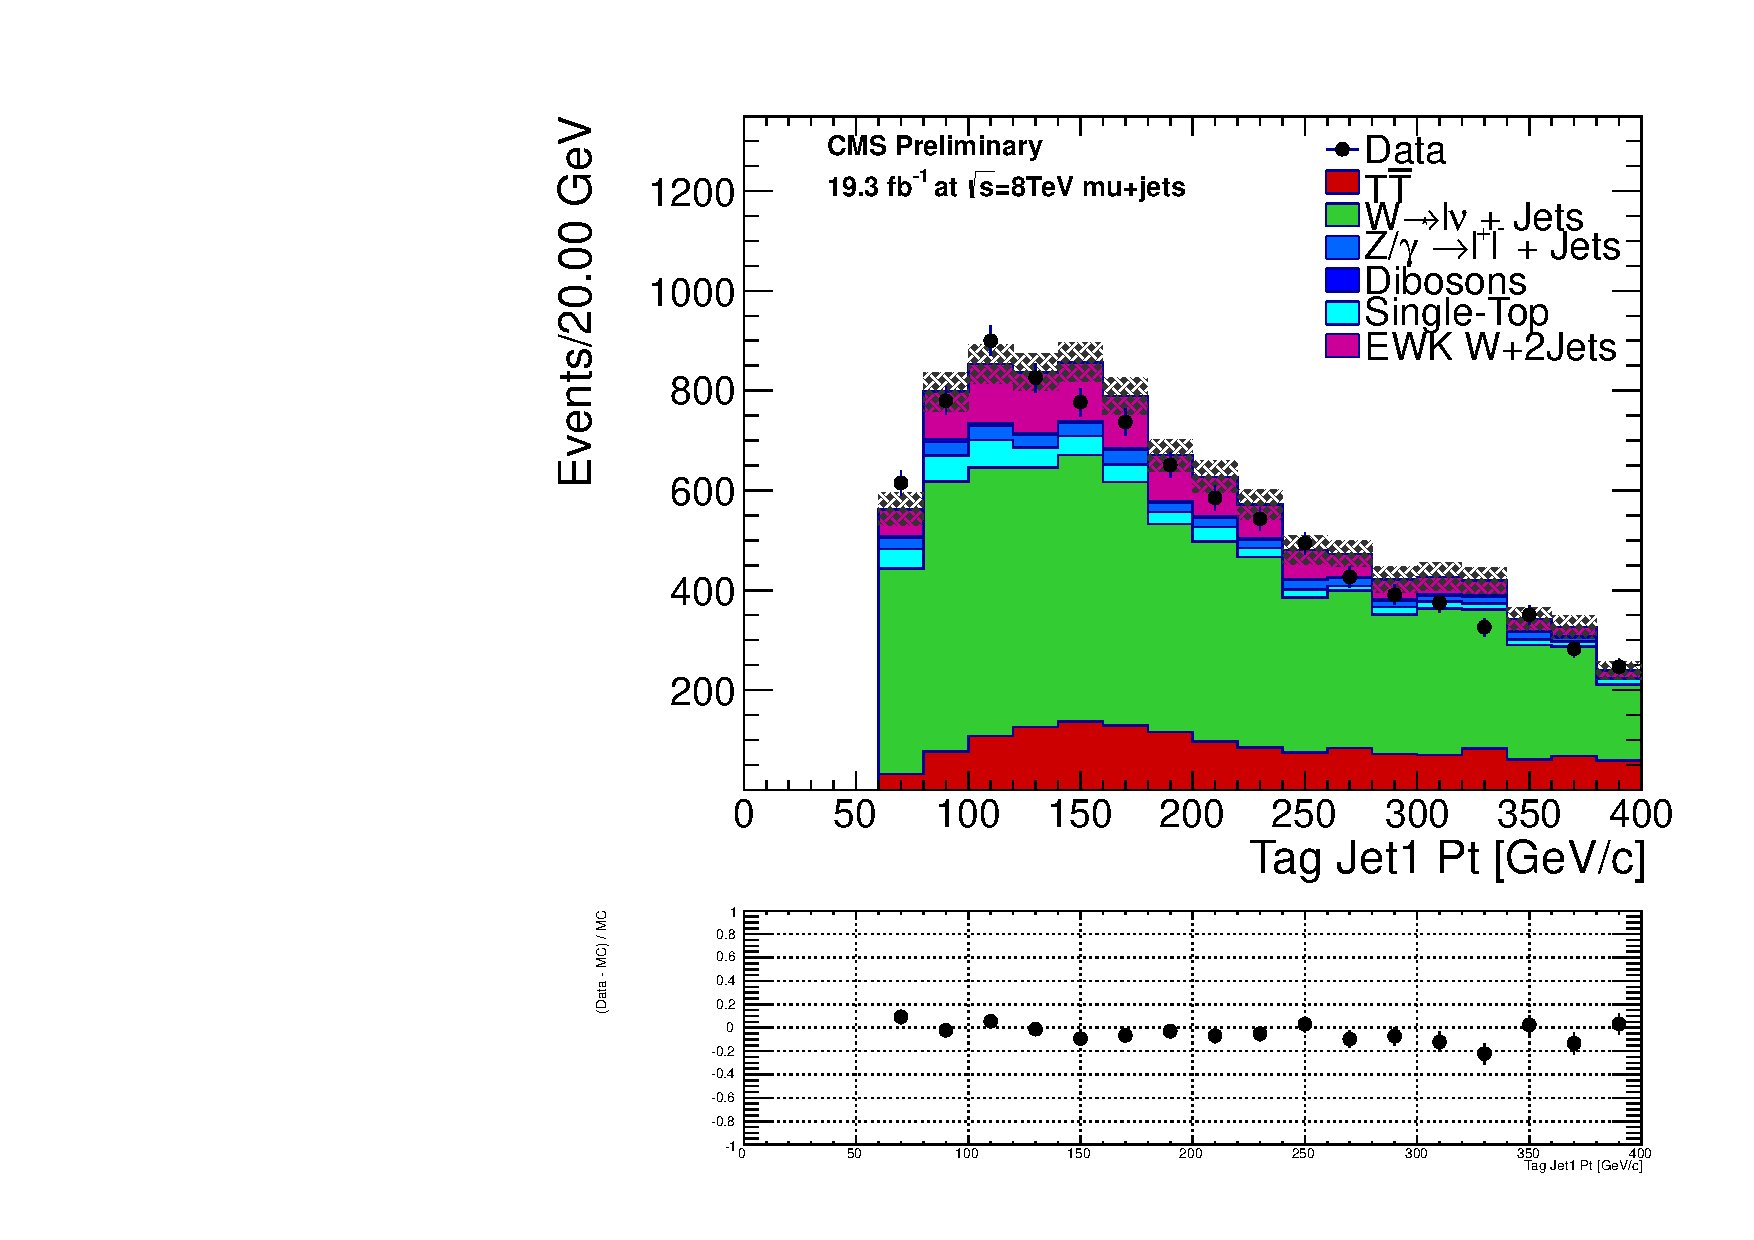
\includegraphics[width=0.49\textwidth]{figs/puchecks/mu_EWK_W_2jets_tagjet1_pt_mjj_600_tagjet1_60_tagjet2_50_Zeppenfield_1point2_nPV_12_EWKW2jets.pdf}
    \includegraphics[width=0.49\textwidth]{figs/puchecks/el_EWK_W_2jets_tagjet1_pt_mjj_600_tagjet1_60_tagjet2_50_Zeppenfield_1point2_nPV_12_met_30_WmT_30_EWKW2jets.pdf}
    \caption{Comparison of the distributions from data and MC of the
    leading jet $p_T$ for muons (left) and electrons (right)
    in Low (NPV$<12$) PileUp events.}
\label{fig:pu_jetldLow}}
\end{figure}
%%%%%%%
%%%%%%%
\begin{figure}[h!t]
  {\centering
    \includegraphics[width=0.49\textwidth]{figs/puchecks/mu_EWK_W_2jets_tagjet1_pt_mjj_600_tagjet1_60_tagjet2_50_Zeppenfield_1point2_nPV_large_12_EWKW2jets.pdf}
    \includegraphics[width=0.49\textwidth]{figs/puchecks/el_EWK_W_2jets_tagjet1_pt_mjj_600_tagjet1_60_tagjet2_50_Zeppenfield_1point2_nPV_large_12_met_30_WmT_30_EWKW2jets.pdf}
    \caption{Comparison of the distributions from data and MC of the
    leading jet $p_T$ for muons (left) and electrons (right)
    in High (NPV$>12$) PileUp events.}
\label{fig:pu_jetldHigh}}
\end{figure}
%%%%%%%
%%%%%%% jetld
\begin{figure}[h!t]
  {\centering
    \includegraphics[width=0.49\textwidth]{figs/puchecks/mu_EWK_W_2jets_tagjet2_pt_mjj_600_tagjet1_60_tagjet2_50_Zeppenfield_1point2_nPV_12_EWKW2jets.pdf}
    \includegraphics[width=0.49\textwidth]{figs/puchecks/el_EWK_W_2jets_tagjet2_pt_mjj_600_tagjet1_60_tagjet2_50_Zeppenfield_1point2_nPV_12_met_30_WmT_30_EWKW2jets.pdf}
    \caption{Comparison of the distributions from data and MC of the
    second leading jet $p_T$ for muons (left) and electrons (right)
    in Low (NPV$<12$) PileUp events.}
\label{fig:pu_jet2ldLow}}
\end{figure}
%%%%%%%
%%%%%%%
\begin{figure}[h!t]
  {\centering
    \includegraphics[width=0.49\textwidth]{figs/puchecks/mu_EWK_W_2jets_tagjet2_pt_mjj_600_tagjet1_60_tagjet2_50_Zeppenfield_1point2_nPV_large_12_EWKW2jets.pdf}
    \includegraphics[width=0.49\textwidth]{figs/puchecks/el_EWK_W_2jets_tagjet2_pt_mjj_600_tagjet1_60_tagjet2_50_Zeppenfield_1point2_nPV_large_12_met_30_WmT_30_EWKW2jets.pdf}
    \caption{Comparison of the distributions from data and MC of the
    second leading jet $p_T$ for muons (left) and electrons (right)
    in High (NPV$>12$) PileUp events.}
\label{fig:pu_jet2ldHigh}}
\end{figure}
%%%%%%%
%%%%%%%%%%%%%%%%%%%%%%%%%%%%
%%%%%%%
%\begin{figure}[h!t]
%  {\centering
%    \includegraphics[width=0.49\textwidth]{figs/puchecks/mu_LowNPV_GroomedJet_mass.png}
%    \includegraphics[width=0.49\textwidth]{figs/puchecks/el_LowNPV_GroomedJet_mass.png}
%    \caption{Comparison of the distributions from data and MC of the
%    merged jet mass for muons (left) and electrons (right)
%    in Low (NPV$<12$) PileUp boosted events.}
%\label{fig:pu_GroomedJet_massLow}}
%\end{figure}
%%%%%%%%
%%%%%%%%
%\begin{figure}[h!t]
%  {\centering
%    \includegraphics[width=0.49\textwidth]{figs/puchecks/mu_MedNPV_GroomedJet_mass.png}
%    \includegraphics[width=0.49\textwidth]{figs/puchecks/el_MedNPV_GroomedJet_mass.png}
%    \caption{Comparison of the distributions from data and MC of the
%    merged jet mass for muons (left) and electrons (right)
%    in Medium ($12<$NPV$<18$) PileUp boosted events.}
%\label{fig:pu_GroomedJet_massMed}}
%\end{figure}
%%%%%%%%
%%%%%%%%
%\begin{figure}[h!t]
%  {\centering
%    \includegraphics[width=0.49\textwidth]{figs/puchecks/mu_HighNPV_GroomedJet_mass.png}
%    \includegraphics[width=0.49\textwidth]{figs/puchecks/el_HighNPV_GroomedJet_mass.png}
%    \caption{Comparison of the distributions from data and MC of the
%    merged jet mass for muons (left) and electrons (right)
%    in High (NPV$>18$) PileUp boosted events.}
%\label{fig:pu_GroomedJet_massHigh}}
%\end{figure}
%%%%%%%%
%%%%%%%%
%\begin{figure}[h!t]
%  {\centering
%    \includegraphics[width=0.49\textwidth]{figs/puchecks/mu_LowNPV_GroomedJet_pt_pr.png}
%    \includegraphics[width=0.49\textwidth]{figs/puchecks/el_LowNPV_GroomedJet_pt_pr.png}
%    \caption{Comparison of the distributions from data and MC of the
%    merged jet $p_T$ for muons (left) and electrons (right)
%    in Low (NPV$<12$) PileUp boosted events.}
%\label{fig:pu_mergedjetptLow}}
%\end{figure}
%%%%%%%%
%%%%%%%%
%\begin{figure}[h!t]
%  {\centering
%    \includegraphics[width=0.49\textwidth]{figs/puchecks/mu_MedNPV_GroomedJet_pt_pr.png}
%    \includegraphics[width=0.49\textwidth]{figs/puchecks/el_MedNPV_GroomedJet_pt_pr.png}
%    \caption{Comparison of the distributions from data and MC of the
%    merged jet $p_T$ for muons (left) and electrons (right)
%    in Medium ($12<$NPV$<18$) PileUp boosted events.}
%\label{fig:pu_mergedjetptMed}}
%\end{figure}
%%%%%%%%
%%%%%%%%
%\begin{figure}[h!t]
%  {\centering
%    \includegraphics[width=0.49\textwidth]{figs/puchecks/mu_HighNPV_GroomedJet_pt_pr.png}
%    \includegraphics[width=0.49\textwidth]{figs/puchecks/el_HighNPV_GroomedJet_pt_pr.png}
%    \caption{Comparison of the distributions from data and MC of the
%    merged jet $p_T$ for muons (left) and electrons (right)
%    in High (NPV$>18$) PileUp boosted events.}
%\label{fig:pu_mergedjetptHigh}}
%\end{figure}
%%%%%%%
%%%%%%%%%%%%%%%%%%%%%%%%%%%%

{\bf To account for differences in the number of pile-up events 
compared to the data, the Monte Carlo samples are re-weighted to 
have on-avearge the same pileup distribution.}


%%%%%%%%%%%%%%%%%%%%%%%%%%%%%%%%%%%%%%%%%%%%%%%%%%%%%%%%%%%%%%%%%%%%
%%%%%%%%%%%%%%%%%%%%%%%%%%%%%%%%%%%%%%%%%%%%%%%%%%%%%%%%%%%%%%%%%%%%
%%%%%%%%%%%%%%%%%%%%%%%%%%%%%%%%%%%%%%%%%%%%%%%%%%%%%%%%%%%%%%%%%%%%
%%%%%%%%%%%%%%%%%%%%%%%%%%%%%%%%%%%%%%%%%%%%%%%%%%%%%%%%%%%%%%%%%%%%
%%%%%%%%%%%%%%%%%%%%%%%%%%%%%%%%%%%%%%%%%%%%%%%%%%%%%%%%%%%%%%%%%%%%
%%%%%%%%%%%%%%%%%%%%%%%%%%%%%%%%%%%%%%%%%%%%%%%%%%%%%%%%%%%%%%%%%%%%
%%%%%%%%%%%%%%%%%%%%%%%%%%%%%%%%%%%%%%%%%%%%%%%%%%%%%%%%%%%%%%%%%%%%
\section{Data Driven QCD Estimation}
\label{sec:qcd}

One background comes from QCD multijet events
with one jet passing the lepton criteria as a 'fake'. However, it is
not practical to generate sufficient MC to create a statistically
significant sample that passes the selection criteria. Therefore, we
rely on a data-driven approach in which the isolation-inverted samples
from data, which mirror the QCD background, are used instead.
Specifically, we perform a template fit to data of
the MET distribution in order to obtain the fraction of QCD events in
the data; these templates are from a data-based QCD sample, a
MC-based W+jets sample and MC-based other samples.

The electron QCD sample is obtained by selecting events
in the data with the isolation $>0.3$ (default selection for loose
electrons uses Iso$_{el}<\sim0.2$).  In order to increase statistics
for the QCD sample we also relax the MET cut from 30~GeV to 20~GeV and
remove the restrictions on Electron MVA.
%Fig.~\ref{fig:QCDISOCutsWmTShape} demonstrates that taking $Iso>0.3$
%(rather than simply inverting the isolation cut), relaxing the MET as
%well as the Electron MVA gives us a falling $W_{mT}$ spectrum (as
%opposed to a signal-like one, which contains a peak near
%$W_{mT}=$80~GeV). The MC W+Jets and target data samples are obtained by
%applying the default cuts (Sec~\ref{sec:firstStep}).

The fraction of QCD events in data is then obtained from a
fit to the MET distribution, with the normalizations for three components (
W+jets, QCD and other contributions(including TTbar, SingleTop, Drell-Yan and Diboson)) free to float.
The results for the electrons are shown in Figure~\ref{fig:QCDTemplateFit_MET}. 
However, we inherently have a smaller sample of 
QCD events for the muons. Their relative fraction
is expected to be $<$1\% ({\it e.g.} 0.2\% in 7~TeV data, AN-11-110).
 
%Likewise, the multijet contribution is suppressed in btagged as well as merged configuration and is highly correlated with the V+Jets background.
%We do not require an independent model of the QCD event in the electron btagged, electron boosted and all muon configurations.

For the electron case we implement the above approach. The final fraction of QCD events in data, after accounting for the change in accepatance due to the MET cut,
is $7.9\%$. We conservatively assume a 50\% uncertainty on the QCD yield when fitting the data (Section~\ref{sec:mjj_fit}). 
%We scan the tagjet mass cut from 0 to 100~GeV to cross check the QCD fraction fit result. From the scan fit result in Fig.~\ref{fig:QCDTemplateFit_MET_tagjetscan} and 50\% is conservarive to cover the QCD yield uncertainty when fitting the data (Section~\ref{sec:mjj_fit}).
%Due to this assumption and to account for po crepancies in template modeling, a very
%large uncertainty is conservatively assumed. The final fraction of QCD
%events in data, after accounting for the change in accepatance due to the MET cut,
%is given in Table~\ref{tab:qcdfrac}.

%%%%%%%%%%%%%%%%%%%%%%%%%%%%%
%\begin{table}[bthp]
%\begin{center}
%  \begin{tabular}{l c}
%    \hline  \hline
%     & 2 jets \\
%    \hline  
%    electron  & 18.6 $\pm$ 0.2\% \\
%    muon      & 0.2 $\pm$ 0.4\% \\
%    \hline  \hline
%  \end{tabular}
%\end{center}
%\caption{\label{tab:qcdfrac} Estimates of the percentage of QCD in data (and
%the fit uncertainty) for the muon and electron datasets after selection.}
%\end{table}

%\subsection{QCD Uncertainties}
%\label{sec:qcd_Uncertainty}
%%%%%%%%%%%%%%%%%%%%%%%%%%%%%

%When performing the $m_{jj}$ fit the QCD yield
%is Gaussian-constrained with a mean given by the value shown in
%Table~\ref{tab:qcdfrac}.
%In the case of electrons, the error on the QCD fraction
%is small and we (conservatively) estimate
%the uncertainty to be one half of the expected value. For muons the
%uncertainty is the error on the relative fraction (i.e.,
%0.4\%).
%When obtaining the result for the sum of electron and muon data, the uncertainties
%are combined using the standard error propagation machinery.


%\subsection{Cross-Checks}
%
%In order to ensure that our inverted selection provides a consistent representation of
%QCD events,
%we fit the QCD with a Rayleigh Function: $xe^{-x^2/2(\sigma_0+\sigma_1x)^2}$,
%used during the inclusive cross section measurements~\cite{WZCMS:2010}.
%As can be seen from Fig.~\ref{fig:QCDMETRayleighFit},
%the function accurately fits the overall shape as well as the parameter
%corresponding to the intrinsic MET resolution ($\sigma_0\simeq 12$~GeV).
%
%In addition we compare the above procedure to the fit with the remaining backgrounds included by
%\begin{itemize}
%\item Fixing the relative ratios based on the expected cross sections and fitting with the combination, instead of W+Jets. The resulting fraction of QCD (after correcting for MET acceptance) is $0.160\pm 0.002$.
%\item Fixing the additional backgrounds to their expected values and only allowing W+Jets (and QCD) to float during the fit. The resulting fraction of QCD (after correcting for MET acceptance) is $0.156\pm 0.002$.
%\end{itemize}
%The results (Fig.~\ref{fig:QCDTemplateFit_MET_AllBkgds}) are consistent with the default approach.
%
%We also examine the impact of the QCD selection cuts on W+Jets and $t\bar{t}$ MC events. The comparison is shown in Fig.~\ref{fig:QCDSelectionDataVsNonQCDMC}. The selection procedure does not significantly alter the shapes of the non-QCD distributions ({\it i.e} we retain the peak near $W_{mT}=$80~GeV and observe a broad resonance, rather than an exponentially falling spectrum, in the MET), which remain distinct from multijet events. There is no evidence that the data sideband contains a significant fraction of non-QCD events. 
%

%%%%%%%%%%%%%%%%%%%%%%%%%%%%
%\begin{figure}[h!] {\centering
%\unitlength=0.33\linewidth
%\includegraphics[width=0.50\textwidth]{figs/qcd/QCD_El_QCDWJets_EWK_W_2jets_W_mT_WmT.pdf}
%\caption{QCD W transverse mass shapes with Iso$>0.3$, MET$>20$ and no Electron MVA cut vs inverted loose isolation, MET$>30$ and loose Electron MVA cuts.}
%\label{fig:QCDISOCutsWmTShape}
%}
%\end{figure}
%%%%%%%
\begin{figure}[h!] {\centering
\unitlength=0.50\linewidth
\includegraphics[width=0.50\textwidth]{figs/qcd/elconstrainotherprocess_event_met_pfmetqcdfittagjetcutWmT30cutmetcut1000_000000_qcdfraction.pdf}
\caption{MET distributions fit for electrons.}
\label{fig:QCDTemplateFit_MET}
}
\end{figure}
%%%%%%%
%\begin{figure}[h!] {\centering
%\unitlength=0.33\linewidth
%\includegraphics[width=0.50\textwidth]{figs/qcd/qcdextrapolationfit.pdf}
%\caption{MET distributions fit to the QCD and W$jj$ templates for electrons by scanning the tag jet pair invariant mass cut.}
%\label{fig:QCDTemplateFit_MET_tagjetscan}
%}
%\end{figure}
%%%%%%%
%\begin{figure}[h!] {\centering
%\unitlength=0.33\linewidth
%\includegraphics[width=0.90\textwidth]{figs/qcd/RaileighFitQCD_19p2fb_el2j.png}
%\caption{QCD MET distribution fitted with a Rayleigh Function.}
%\label{fig:QCDMETRayleighFit}
%}
%\end{figure}
%%%%%%%%
%%%%%%%%
%\begin{figure}[h!] {\centering
%\unitlength=0.33\linewidth
%\includegraphics[width=0.90\textwidth]{figs/qcd/El2J_19p2fb_CutComparison_WmT.png}
%% \put(-0.80,0.0){(a)}
%% \unitlength=0.33\linewidth
%% \includegraphics[width=0.48\textwidth]{figs/2012_QCD/ISOShapeComp_WmT_mu3j_g01vg02.pdf}
%% \put(-0.80,0.0){(b)} \\
%% \unitlength=0.33\linewidth
%% \includegraphics[width=0.48\textwidth]{figs/2012_QCD/ISOShapeComp_WmT_el2j_g01vg02.pdf}
%% \put(-0.80,0.0){(c)}
%% \unitlength=0.33\linewidth
%% \includegraphics[width=0.48\textwidth]{figs/2012_QCD/ISOShapeComp_WmT_el3j_g01vg02.pdf}
%% \put(-0.80,0.0){(d)}
%\caption{ QCD W transverse mass shapes with Iso$>0.3$, MET$>20$ and no Electron MVA cut vs inverted loose isolation, MET$>30$ and loose Electron MVA cuts.}
%\label{fig:QCDISOCutsWmTShape}
%}
%\end{figure}
%%%%%%%%
%%%%%%%%
%\begin{figure}[h!] {\centering
%\unitlength=0.33\linewidth
%\includegraphics[width=0.48\textwidth]{figs/qcd/TemplateFit19p2fb_MET_AllBkgds_el2j.png}
%\put(-0.80,0.0){(a)}
%\unitlength=0.33\linewidth
%\includegraphics[width=0.48\textwidth]{figs/qcd/TemplateFit19p2fb_MET_AllBkgdsFixNonWpJ_el2j.png}
%\put(-0.80,0.0){(b)}
%\caption{ Electron MET distribution fit with: (a) fractions of the non QCD processes fixed relative to each other and the overall coefficient allowed to float (b) the additional backgrounds (i.e. processes which are not W+Jets or QCD) fixed to their expected yields and W+Jets (as well as QCD) fraction allowed to float. The resultant fraction of QCD events is consistent with the default approach (Fig.~\ref{fig:QCDTemplateFit_MET}).}
%\label{fig:QCDTemplateFit_MET_AllBkgds}}
%\end{figure}
%%%%%%%%
%%%%%%%%
%\begin{figure}[h!] {\centering
%\unitlength=0.33\linewidth
%\includegraphics[width=0.48\textwidth]{figs/qcd/El2J_11p9fb_QCDvsMC_WmT.png}
%\put(-0.80,0.0){(a)}
%\unitlength=0.33\linewidth
%\includegraphics[width=0.48\textwidth]{figs/qcd/El2J_11p9fb_QCDvsMC_MET.png}
%\put(-0.80,0.0){(b)}
%\caption{ Data, W+Jets MC and $t\bar{t}$ MC events with Iso$>0.3$, MET$>20$ and no Electron MVA cut for (a) $W_{mT}$ (b) MET. The shapes are distinct and there is no evidence of contamination in (what should be) data sideband multijet events.}
%\label{fig:QCDSelectionDataVsNonQCDMC}}
%\end{figure}
%%%%%%%%


%%%%%%%%%%%%%%%%%%%%%%%%%%%%%%%%%%%%%%%%%%%%%%%%%%%%%%%%%%%%%%%%%%
%%%%%%%%%%%%%%%%%%%%%%%%%%%%%%%%%%%%%%%%%%%%%%%%%%%%%%%%%%%%%%%%%%
%%%%%%%%%%%%%%%%%%%%%%%%%%%%%%%%%%%%%%%%%%%%%%%%%%%%%%%%%%%%%%%%%%

\clearpage
%\section{W+jets Background}
%\label{sec:wjetsBackground}
%
%In order to get a good description of the W+jets shape in data, the
%simulation needs to describe well both the matrix elements for the
%hard processes, and the subsequent development of the hard partons
%into jets of hadrons.  However, no factorization theorem exists to
%rigorously separate these two components.  A given (n + 1)-jet event
%can be obtained in two ways: from the collinear/soft-radiation
%evolution of an appropriate (n + 1)-parton final state, or from an
%n-parton configuration where hard, large-angle emission during its
%evolution leads to the extra jet.  A factorization scheme defines, on
%an event-by-event basis, which of the two paths should be followed.
%The two relevant parameters defining such a scheme are: the
%factorization/renormalization scale $q^2$ and the matrix element -
%parton shower matching threshold.  Optimized values of these
%parameters should give the best possible approximation to the W+jets
%kinematics for a given fixed-order calculation.  We know that the
%physics has to be independent of the relative contributions of the two
%components.
%
%The CMS MadGraph W+jets production uses MLM matching
%\cite{Hoche:2006ph} with $k_T$ jets.  The default matching threshold
%is 10~GeV (i.e., if the parton $p_{T}$ is greater than 10~GeV, then it
%is assumed to have originated from the hard scattering process and
%contributes to the matrix element calculation; if the parton $p_{T}$
%is less than 10~GeV then it is assumed to come from the parton
%shower).  The factorization/renormalization scale $q^2$ corresponds to
%the ``transverse mass'' of the W boson plus the hard jets: $\sqrt{M_W^2 + p_{T, W}^2 + \Sigma p_{T,j}^2}$.
%
%\subsection{Factorization/renormalization scale and matrix element - parton shower matching threshold}
%\label{sec:wjetsShapeMatchingQ2}
%
%To perform studies of the uncertainty due to the choice of the $q^2$
%and matching scales, alternative MadGraph W+jets samples are produced
%in which the corresponding scales are changed by a factor of 2. Thus,
%we have ``matching-up'', ``matching-down'', ``scale-up'', and
%``scale-down'' samples, each yielding an $m_{jj}$ distribution, or
%template. In order to compensate for limited statistics in the centrally generated samples
%additional MadGraph Monte Carlo is produced locally with (the majority of) selection cuts applied at the generation level.
%The approach significantly reduces the amount of MC required, though running the full detector simulation remaings a computing intensive process. In the end we generate enough events to effectively double the size of the samples and use the combination of local plus central ones, added with equal weights, in subsequent studies. All these four samples have low statistics after applying the selection cuts and are not used in the fit to extract the electroweak W+2jets signal.
%%First, we attempt to follow the 7~TeV approach by using our samples to find an optimum MC template
%$\mathcal{F}_{W+\text{jets}}$,
%%%\[
%\begin{equation}
%\mathcal{F}_{W+\text{jets}} = \sum_\alpha f_\alpha \mathcal{G}_\alpha\, + (1-\sum_\alpha f_\alpha)\times\mathcal{G}_\text{nominal},
%\label{eqn:wjetsShapeMatchingQ2}
%\end{equation}
%%%\]
%where $\alpha \in
%\{\text{matchingUp,~matchingDown,~scaleUp,~scaleDown}\}$,
%$\mathcal{G}_\text{nominal}$ is the template from the default MadGraph
%generation and $\mathcal{G}_\alpha$ is the template from the specified
%sample.  We define a 2D coordinate system in scale and matching.  The
%origin corresponds to the default MadGraph sample.  To move in the
%positive scaleUp direction, one sets $f_\text{scaleDown}=0$ and
%increases $f_\text{scaleUp}$. To move in the negative scaleUp
%direction, one sets $f_\text{scaleUp}=0$ and increases
%$f_\text{scaleDown}$.  The same is true for the matching samples.  We
%allow the relative contributions from these templates to float in our
%fit.  This lets the data determine the best W+jets shape and the
%uncertainties on these parameters is automatically propagated to the
%uncertainties on the yields.
%
%
%\subsection{Monte Carlo Template Fit}
%
%We follow the usual approach (described in section~\ref{sec:mjj_fit}) obtaining the diboson signal yield from an unbinned maximum
%likelihood fit to the dijet invariant mass distribution in the data. The exctracted fraction (of the expected Standard Model diboson yield) is $1.74\pm 0.18$ ($2.11\pm 0.26$) in the muon (electron) channel. Likewise, the fit results (Figs.~\ref{fig:mjjfit_MCTemplate_mu},~\ref{fig:mjjfit_MCTemplate_el}) show a mismatch between the MC fit output and the data along with the corresponding bias in the pull distributions.
%
%%%%%%%%%%%%%%%%%%%%%
%\begin{figure}[h!]
%  {\centering
%    \includegraphics[width=0.49\textwidth]{figs/mjjfit/DibosonMCTemplatelnujj_muon_Stacked.png}
%    \includegraphics[width=0.49\textwidth]{figs/mjjfit/DibosonMCTemplatelnujj_muon_Subtracted.png}
%    \includegraphics[width=0.49\textwidth]{figs/mjjfit/DibosonMCTemplatelnujj_muon_Pull.png}
%    \caption{Distribution of the W-jet invariant mass for the dijet (anti-btagged) 2+ jet events in muon data and fit shapes: 
%      (upper left) All background components stacked together, 
%      (upper right) unstacked, (lower left) [Data minus all backgrounds except diboson],  
%      (lower right) normalized residual between data and MC. The vertical dotted lines
%      indicate the mass interval excluded from the fit. The shape templates for each component are taken directly from Monte Carlo.}
%    \label{fig:mjjfit_MCTemplate_mu}}
%\end{figure}
%%%%%%%%%%%%%%%%%%%%%
%%%%%%%%%%%%%%%%%%%%%
%\begin{figure}[h!]
%  {\centering
%    \includegraphics[width=0.49\textwidth]{figs/mjjfit/DibosonMCTemplatelnujj_electron_Stacked.png}
%    \includegraphics[width=0.49\textwidth]{figs/mjjfit/DibosonMCTemplatelnujj_electron_Subtracted.png}
%    \includegraphics[width=0.49\textwidth]{figs/mjjfit/DibosonMCTemplatelnujj_electron_Pull.png}
%    \caption{Distribution of the W-jet invariant mass for the dijet (anti-btagged) 2+ jet events in electron data and fit shapes: 
%      (upper left) All background components stacked together, 
%      (upper right) unstacked, (lower left) [Data minus all backgrounds except diboson],  
%      (lower right) normalized residual between data and MC. The vertical dotted lines
%      indicate the mass interval excluded from the fit. The shape templates for each component are taken directly from Monte Carlo.}
%    \label{fig:mjjfit_MCTemplate_el}}
%\end{figure}
%%%%%%%%%%%%%%%%%%%%%


%\subsection{Convolved Monte Carlo Template Fit}
%\label{sec:convolvedMCfit}
%
%Next, we include the resolution effects directly in our fit (rather than treating them as a separate systematics). We take the gaussian resolution function, obtained from fits to the top control sample (section~\ref{sec:convolvedMCfit}), convolve it with the MC templates and repeat the fit. The results are shown in Figs.~\ref{fig:mjjfit_ConvolvedMCTemplate_mu},~\ref{fig:mjjfit_ConvolvedMCTemplate_el} with the extracted fraction (of the expected Standard Model diboson yield) of $1.71\pm 0.18$. The plots show a mismatch between MC fit output and the data along with the corresponding bias in the pull distributions. Accounting for resolution effects has a minimal impact on the fitting procedure. The above approach is inadequate for modeling the dijet mass distribution in the full 8~TeV CMS dataset.
%
%%%%%%%%%%%%%%%%%%%%%
%\begin{figure}[h!]
%  {\centering
%    \includegraphics[width=0.49\textwidth]{figs/mjjfit/DibosonConvolvedMCTemplatelnujj_muon_Stacked.png}
%    \includegraphics[width=0.49\textwidth]{figs/mjjfit/DibosonConvolvedMCTemplatelnujj_muon_Subtracted.png}
%    \includegraphics[width=0.49\textwidth]{figs/mjjfit/DibosonConvolvedMCTemplatelnujj_muon_Pull.png}
%    \caption{Distribution of the W-jet invariant mass for the dijet (anti-btagged) 2+ jet events in muon data and fit shapes: 
%      (upper left) All background components stacked together, 
%      (upper right) unstacked, (lower left) [Data minus all backgrounds except diboson],  
%      (lower right) normalized residual between data and MC. The vertical dotted lines
%      indicate the mass interval excluded from the fit. The shape templates for each component are taken directly from Monte Carlo.}
%    \label{fig:mjjfit_ConvolvedMCTemplate_mu}}
%\end{figure}
%%%%%%%%%%%%%%%%%%%%%
%%%%%%%%%%%%%%%%%%%%%
%\begin{figure}[h!]
%  {\centering
%    \includegraphics[width=0.49\textwidth]{figs/mjjfit/DibosonConvolvedMCTemplatelnujj_electron_Stacked.png}
%    \includegraphics[width=0.49\textwidth]{figs/mjjfit/DibosonConvolvedMCTemplatelnujj_electron_Subtracted.png}
%    \includegraphics[width=0.49\textwidth]{figs/mjjfit/DibosonConvolvedMCTemplatelnujj_electron_Pull.png}
%    \caption{Distribution of the W-jet invariant mass for the dijet (anti-btagged) 2+ jet events in electron data and fit shapes: 
%      (upper left) All background components stacked together, 
%      (upper right) unstacked, (lower left) [Data minus all backgrounds except diboson],  
%      (lower right) normalized residual between data and MC. The vertical dotted lines
%      indicate the mass interval excluded from the fit. The shape templates for each component are taken directly from Monte Carlo.}
%    \label{fig:mjjfit_ConvolvedMCTemplate_el}}
%\end{figure}
%%%%%%%%%%%%%%%%%%%%%


%\clearpage
%\section{Modeling Individual Processes}
%\subsection{V+jets Background Shape}
%\label{sec:wjetsShape}
%
%Because of inadequate statistics in the V+jets MC and the overall poor
%agreement between V+jets MC and many data distibutions, we employ an
%empirical description of the V+jets shape for the default MadGraph sample, which consists of W+jets based on their predicted cross-sections(Table~\ref{tab:bkg_XS}). In the signal regime the two parameter power law function is used:%, modulated by the error function corresponding to a kinematic turnon, for the anti-btagged events:
%\begin{equation}
%  %\mathcal{F}_{V+\text{jets}} = \text{erf}(m_{jj}; m_0, \sigma)\times\left[(m_{jj})^{-\alpha-\beta\ln(m_{jj}/\sqrt{s})}\right]
%   \mathcal{F}_{V+\text{jets}} =  \frac{1.0}{m_{jj}^{a_{0} + a_{1}log(m_{jj}/8000)}}
%\end{equation}
%where $a_{0}$ and $a_{1}$ paramters determined from the fit.
%%and a simple power law (modulated by the error function) for the btagged events:
%%\begin{equation}
%%  \mathcal{F}_{V+\text{jets}} = \text{erf}(m_{jj}; m_0, \sigma)\times\left[(m_{jj})^{-\alpha}\right]\,,
%%\end{equation}
%%where $m_0$ and $\sigma$, corresponding to the value and the width of this turn on, are determined from the fit (as are $\alpha$ and $\beta$). %For the boosted events the shape is modeled by the error function times an exponential falloff:
%%\begin{equation}
%%  \mathcal{F}_{V+\text{Jet}} = \text{erf}(m_{J}; m_0, \sigma)\times e^{-\alpha m_{J}}\,,
%%\end{equation}
%%with the parameters determined from the fit. 
%More specifically, the parameters are determined from the fit to the Monte Carlo and are then allowed Wjets shape paramters to vary. The parameter values along with corresponding constraints are listed in Table~\ref{tab:FloatingShapePars}. In Figs.~\ref{fig:WpJFit_Dijet} we show the result of an unbinned maximum likelihood fit to the MC distributions. As can be seen, there is a good agreement between projection and the simulation.
%
%%%%%%%%%%%%%%%%
%\begin{table}[bthp]
%\begin{center}
%\caption{Shape parameters floating during the fit to the data.}
% \label{tab:FloatingShapePars}
%\vspace{0.5cm}
% \begin{tabular} {l  c  c c c }
%   \hline 
%\hline
%Parameter            &  \multicolumn{2}{c}{Muons} & \multicolumn{2}{c}{Electrons} \\  
%\hline
%               & Central Value &   Uncertainty     &  Central Value &  Uncertainty \\
%\hline
%W+Jets $a_{0}$          &               &                &                &              \\
%\hline
%W+Jets $a_{1}$       &              &                   &                &              \\
%\hline
%\hline
%\end{tabular}
%\end{center}
%\end{table}
%%%%%%%%%%%%%%%%
%
%%When fitting the dijet mass spectrum we implement the procedure described above (Eq.~\ref{eqn:wjetsShapeMatchingQ2}) with the empirical shape used in place of the default sample, while t%he factorization/renormalization and matrix element - parton shower matching templates come from the simulation. The parameters of the polynomial are allowed to vary subject to gaussian %constraints from the MC fit. In the boosted case there are no alternate samples available and we allow the parameters (for both the core and tail gaussians) to vary freely during the fit% to the data.
%
%\begin{figure}
%\begin{center}
%\includegraphics[width=0.45\textwidth]{figs/wpj/EWKW2jetstagjetmjj_WpJ_muon_Model_12_Validate.png}
%\includegraphics[width=0.45\textwidth]{figs/wpj/EWKW2jetstagjetmjj_WpJ_electron_Model_12_Validate.png}
%\end{center}
%\caption{\label{fig:WpJFit} V+jets $m_{jj}$ tag jet pair mass shape:
%Projection of a fit to the V+jets MC for muons (left) and electrons (right).}
%\label{fig:WpJFit_Dijet}
%\end{figure}
%
%\begin{figure}
%\begin{center}
%\includegraphics[width=0.45\textwidth]{figs/wpj/EWKW2jetstagjetmjj_WpJ_muon_Model_12_Validate_pull.png}
%\includegraphics[width=0.45\textwidth]{figs/wpj/EWKW2jetstagjetmjj_WpJ_electron_Model_12_Validate_pull.png}
%\end{center}
%\caption{\label{fig:WpJFit} V+jets $m_{jj}$ tag jet pair mass shape:
%Pull distribution of a fit to the V+jets MC for muons (left) and electrons (right).}
%\label{fig:WpJFit_Dijet_Pull}
%\end{figure}
%
%\subsubsection{Matrix Element - Parton Shower Matching And Factorization/Renormalization Scale Uncertainties}
%The potential V+Jets shape variations due to the choice of ME-PS Matching and Factorization/Renormalization scales are accounted for using the corresponding samples (described in section~\ref{sec:wjetsShapeMatchingQ2}). Due to limited statistic of ME-PS Matching and Factorization/Renormalization scales systematic samples, we don't use these samples. In oder to account for mismodeling of Wjets background shape, we float the Wjets shape parameter in the fit.
%%For the anti-btagged dijet case (where the fit could potentially be sensitive to such fluctuations) we fit each of the alternate samples with the V+Jets parametric shape (Figs.~\ref{fig:WpJAlternateScaleSampleFit_Dijet_mu},~\ref{fig:WpJAlternateScaleSampleFit_Dijet_el}), compare the differences with the default MC fit result above and increase the error when needed. Specifically, for a each parameter the default value is compared to the one returned by the alternate fit ($\pm$ statistical fluctuations due to a limited amount of events in the alternate samples); and the difference between the two is treated as the error, provided it is greater than the uncertainty returned by the default fit. The comparison is made for each of the four alternate samples, while we take the maximum of the four to be the new fit error. While the 8~TeV analysis relies on parametric shapes (rather than templates taken directly from the Monte Carlo) the concept behind our treatment of alternate scale uncertainties is the same: the fit accounts for the uncertainties due to the choice of ME-PS Matching and Factorization/Renormalization scales by selecting the optimal shape based on the data.
%
%%%%%%%%%%%%%%%%%%%%%
%%%%%%%%
%%\begin{figure}[h!] {\centering
%%\unitlength=0.33\linewidth
%%\includegraphics[width=0.48\textwidth]{figs/wpj/WpJDibosonParametersMU_mu_compFit.png}
%%\put(-0.80,0.0){(a)} 
%%\unitlength=0.33\linewidth
%%\includegraphics[width=0.48\textwidth]{figs/wpj/WpJDibosonParametersMD_mu_compFit.png}
%%\put(-0.80,0.0){(b)}\\
%%\unitlength=0.33\linewidth
%%\includegraphics[width=0.48\textwidth]{figs/wpj/WpJDibosonParametersSU_mu_compFit.png}
%%\put(-0.80,0.0){(c)}
%%\unitlength=0.33\linewidth
%%\includegraphics[width=0.48\textwidth]{figs/wpj/WpJDibosonParametersSD_mu_compFit.png}
%%\put(-0.80,0.0){(d)}
%%\caption{Alternate ME-PS Matching and Factorization/Renormalization scale sample fit of the W+jets $m_{jj}$ shape for the dijet (non-boosted, anti-btagged) muon events. Projection of a fit to the V+jets for: (a) Matching Up, (b) Matching Down, (c) Scale Up, (d) Scale Down MC.} 
%%\label{fig:WpJAlternateScaleSampleFit_Dijet_mu}}
%%\end{figure}
%%%%%%%%%
%%%%%%%%%
%%\begin{figure}[h!] {\centering
%%\unitlength=0.33\linewidth
%%\includegraphics[width=0.48\textwidth]{figs/wpj/WpJDibosonParametersMU_el_compFit.png}
%%\put(-0.80,0.0){(a)} 
%%\unitlength=0.33\linewidth
%%\includegraphics[width=0.48\textwidth]{figs/wpj/WpJDibosonParametersMD_el_compFit.png}
%%\put(-0.80,0.0){(b)}\\
%%\unitlength=0.33\linewidth
%%\includegraphics[width=0.48\textwidth]{figs/wpj/WpJDibosonParametersSU_el_compFit.png}
%%\put(-0.80,0.0){(c)}
%%\unitlength=0.33\linewidth
%%\includegraphics[width=0.48\textwidth]{figs/wpj/WpJDibosonParametersSD_el_compFit.png}
%%\put(-0.80,0.0){(d)}
%%\caption{Alternate ME-PS Matching and Factorization/Renormalization scale sample fit of the W+jets $m_{jj}$ shape for the dijet (non-boosted, anti-btagged) electron events. Projection of a fit to the V+jets for: (a) Matching Up, (b) Matching Down, (c) Scale Up, (d) Scale Down MC.} 
%%\label{fig:WpJAlternateScaleSampleFit_Dijet_el}}
%%\end{figure}
%%%%%%%%
%%%%%%%%%%%%%%%%%%%%%%%%%
%
%
%\subsection{Diboson Shape}
%Likewise, we use a parametric shape to model the diboson signal. The sample itself is a combination of the WW, WZ and ZZ processes (combined in MC based on their expected cross sections). We also use a two parameter power law function to discribe the diboson shape: 
%%a sum of two gaussians (corresponding to the W and Z) separated by a fixed offset (10.8~GeV) and an exponential tail modulated by an error function to parameterize both the dijet and the boosted distributions:
%\begin{equation}
%   \mathcal{F}_{diboson} =  \frac{1.0}{m_{jj}^{a_{0} + a_{1}log(m_{jj}/8000)}}
%\end{equation}
%where $a_{0}$ and $a_{1}$ paramters determined from the fit.
%%where $f_{W}$, $f_{Z}$, $m_{W}$, $m_0$, $\sigma_0$ and $\alpha$ are fixed based on the Monte Carlo. The value for the resolution ($\sigma$) is also obtained from the fit to the MC, but is inflated by a factor of 1.11 to account for the discrepancy between data and MC, based on control sample studies. 
%The results of the parametric shape fit to the simulation are displayed in Figs.~\ref{fig:dibosonFit_Dijet},~\ref{fig:dibosonFit_Dijet_Pull} and show a good level of agreement between the two.
%
%\begin{figure}
%\begin{center}
%\includegraphics[width=0.45\textwidth]{figs/wpj/EWKW2jetstagjetmjj_diboson_muon_Model_12_Validate.png}
%\includegraphics[width=0.45\textwidth]{figs/wpj/EWKW2jetstagjetmjj_diboson_electron_Model_12_Validate.png}
%\end{center}
%\caption{\label{fig:dibosonFit} Diboson $m_{jj}$ tag jet pair mass shape: projection of a fit to the diboson MC for muons (left) and electrons (right).}
%\label{fig:dibosonFit_Dijet}
%\end{figure}
%
%\begin{figure}
%\begin{center}
%\includegraphics[width=0.45\textwidth]{figs/wpj/EWKW2jetstagjetmjj_diboson_muon_Model_12_Validate_pull.png}
%\includegraphics[width=0.45\textwidth]{figs/wpj/EWKW2jetstagjetmjj_diboson_electron_Model_12_Validate_pull.png}
%\end{center}
%\caption{\label{fig:dibosonFit} Diboson $m_{jj}$ tag jet pair mass  shape: Pull distribution of a fit to the diboson MC for muons (left) and electrons (right).}
%\label{fig:dibosonFit_Dijet_Pull}
%\end{figure}
%
%\subsection{Top Background Shape}
%The top background is a combination of \ttbar\ and single top processes with the MC samples combined based on the expected cross sections (Table~\ref{tab:bkg_XS}). The shape is also modeled by a two parameter power law function:
%\begin{equation}
%   \mathcal{F}_{Top} =  \frac{1.0}{m_{jj}^{a_{0} + a_{1}log(m_{jj}/8000)}}
%\end{equation}
%where $a_{0}$ and $a_{1}$ paramters determined from the fit.
%%\begin{equation}
%  %\mathcal{F}_{t\bar{t}} = f_{W}\text{Gaus}(m_{jj}; m_{W}, \sigma_{W})+\text{erf}(m_{jj}; m_0, \sigma)\times e^{-\alpha m_{jj}}\,,
%%\end{equation}
%%a third order (Chebyshev) Polynomial for the btagged dijet case and a pair of gaussians plus an exponential times an error function for the boosted case:
%%\begin{equation}
%%  \mathcal{F}_{t\bar{t}} = f_{G}(\text{Gaus}(m_{J}; m_{1}, \sigma_{1})+0.78\text{Gaus}(m_{J}; m_{1}, 4.6\sigma_{1}))+\text{erf}(m_{J}; m_0, \sigma)\times e^{-\alpha m_{J}}\,,
%%\end{equation}
%%where (for the boosted scenario) $\alpha$ is allowed to float in the fit to the data, subject to gaussian constraints obtained from the simulation, and the resolution of the gaussian (corresponding to the W resonance) is inflated by a factor of 1.11 to account for the discrepancy between data and MC, similar to the diboson case. 
%The parameters are obtained from the simulation (Figs.~\ref{fig:topFit_Dijet},~\ref{fig:topFit_Dijet_Pull} are fixed during the fit to the data. We also use other ttbar samples with different generators(1. aMC@NLO+Herwig 2. Powheg+Pythia) to account for the ttbar shape systematic uncertainty(Details in section~\ref{sec:ttbar_resulved}).
%
%\begin{figure}
%\begin{center}
%\includegraphics[width=0.45\textwidth]{figs/wpj/EWKW2jetstagjetmjj_top_muon_Model_12_Validate.png}
%\includegraphics[width=0.45\textwidth]{figs/wpj/EWKW2jetstagjetmjj_top_electron_Model_12_Validate.png}
%\end{center}
%\caption{\label{fig:topFit} Top $m_{jj}$ tag jet pair mass shape: projection of a fit to the top MC for muons (left) and electrons (right).}
%\label{fig:topFit_Dijet}
%\end{figure}
%
%\begin{figure}
%\begin{center}
%\includegraphics[width=0.45\textwidth]{figs/wpj/EWKW2jetstagjetmjj_top_muon_Model_12_Validate_pull.png}
%\includegraphics[width=0.45\textwidth]{figs/wpj/EWKW2jetstagjetmjj_top_electron_Model_12_Validate_pull.png}
%\end{center}
%\caption{\label{fig:topFit} Top $m_{jj}$ tag jet pair mass shape: Pull distribution of a fit to the top MC for muons (left) and electrons (right).}
%\label{fig:topFit_Dijeti_Pull}
%\end{figure}
%
%\subsection{QCD}
%The electron data events contain a significant (\~5\%) contribution from multijet processes. 
%%For the boosted scenario their shape is sufficiently similar to the one for V+jet events to be absorbed by the corresponding parametrization; while 
%A thorough treatment of the QCD background is presented in Section~\ref{sec:qcd}. It is also parametrized by the two parameter power law function:
%\begin{equation}
%   \mathcal{F}_{Top} =  \frac{1.0}{m_{jj}^{a_{0} + a_{1}log(m_{jj}/8000)}}
%\end{equation}
%where $a_{0}$ and $a_{1}$ paramters determined from the fit.
%%The QCD shape for btagged events is sufficiently similar to V+Jets to be absorbed by their parametrization. 
%In case of muons the multijet contribution is negligible.
%
%\begin{figure}
%\begin{center}
%\includegraphics[width=0.45\textwidth]{figs/wpj/EWKW2jetstagjetmjj_QCD_electron_Model_12_Validate.png}
%\end{center}
%\caption{QCD $m_{jj}$ tag jet pair mass shape in the electron sample: projection of a fit to the QCD data driven shape for electrons.}
%\label{fig:QCDFit_Dijet}
%\end{figure}
%
%\subsection{Electroweak W+2jets signal Shape}
%For our signal shape, the two parameter power law function is also used to discribe the MC shape:
%\begin{equation}
%   \mathcal{F}_{EWK W2jets} =  \frac{1.0}{m_{jj}^{a_{0} + a_{1}log(m_{jj}/8000)}}
%\end{equation}
%where $a_{0}$ and $a_{1}$ paramters determined from the fit.
%
%The results of the parametric shape fit to the simulation are displayed in Figs.~\ref{fig:ewkw2jets_Dijet},~\ref{fig:ewkw2jets_Dijet_Pull}).
%\begin{figure}
%\begin{center}
%\includegraphics[width=0.45\textwidth]{figs/wpj/EWKW2jetstagjetmjj_EWKW2jets_muon_Model_12_Validate.png}
%\includegraphics[width=0.45\textwidth]{figs/wpj/EWKW2jetstagjetmjj_EWKW2jets_electron_Model_12_Validate.png}
%\end{center}
%\caption{\label{fig:topFit} EWKW2jets $m_{jj}$ tag jet pair mass shape: projection of a fit to the top MC for muons (left) and electrons (right).}
%\label{fig:ewkw2jets_Dijet}
%\end{figure}
%
%\begin{figure}
%\begin{center}
%\includegraphics[width=0.45\textwidth]{figs/wpj/EWKW2jetstagjetmjj_EWKW2jets_muon_Model_12_Validate_pull.png}
%\includegraphics[width=0.45\textwidth]{figs/wpj/EWKW2jetstagjetmjj_EWKW2jets_electron_Model_12_Validate_pull.png}
%\end{center}
%\caption{\label{fig:topFit} EWKW2jets $m_{jj}$ tag jet pair mass shape: Pull distribution of a fit to the top MC for muons (left) and electrons (right).}
%\label{fig:ewkw2jets_Dijet_Pull}
%\end{figure}

\clearpage
